\label{DOMFits}

\section{DOM fit of \oSix}

\label{O16DOMOutput}
\begin{figure}[H]
    \centering
    \begin{minipage}{0.45\textwidth}
        \centering
        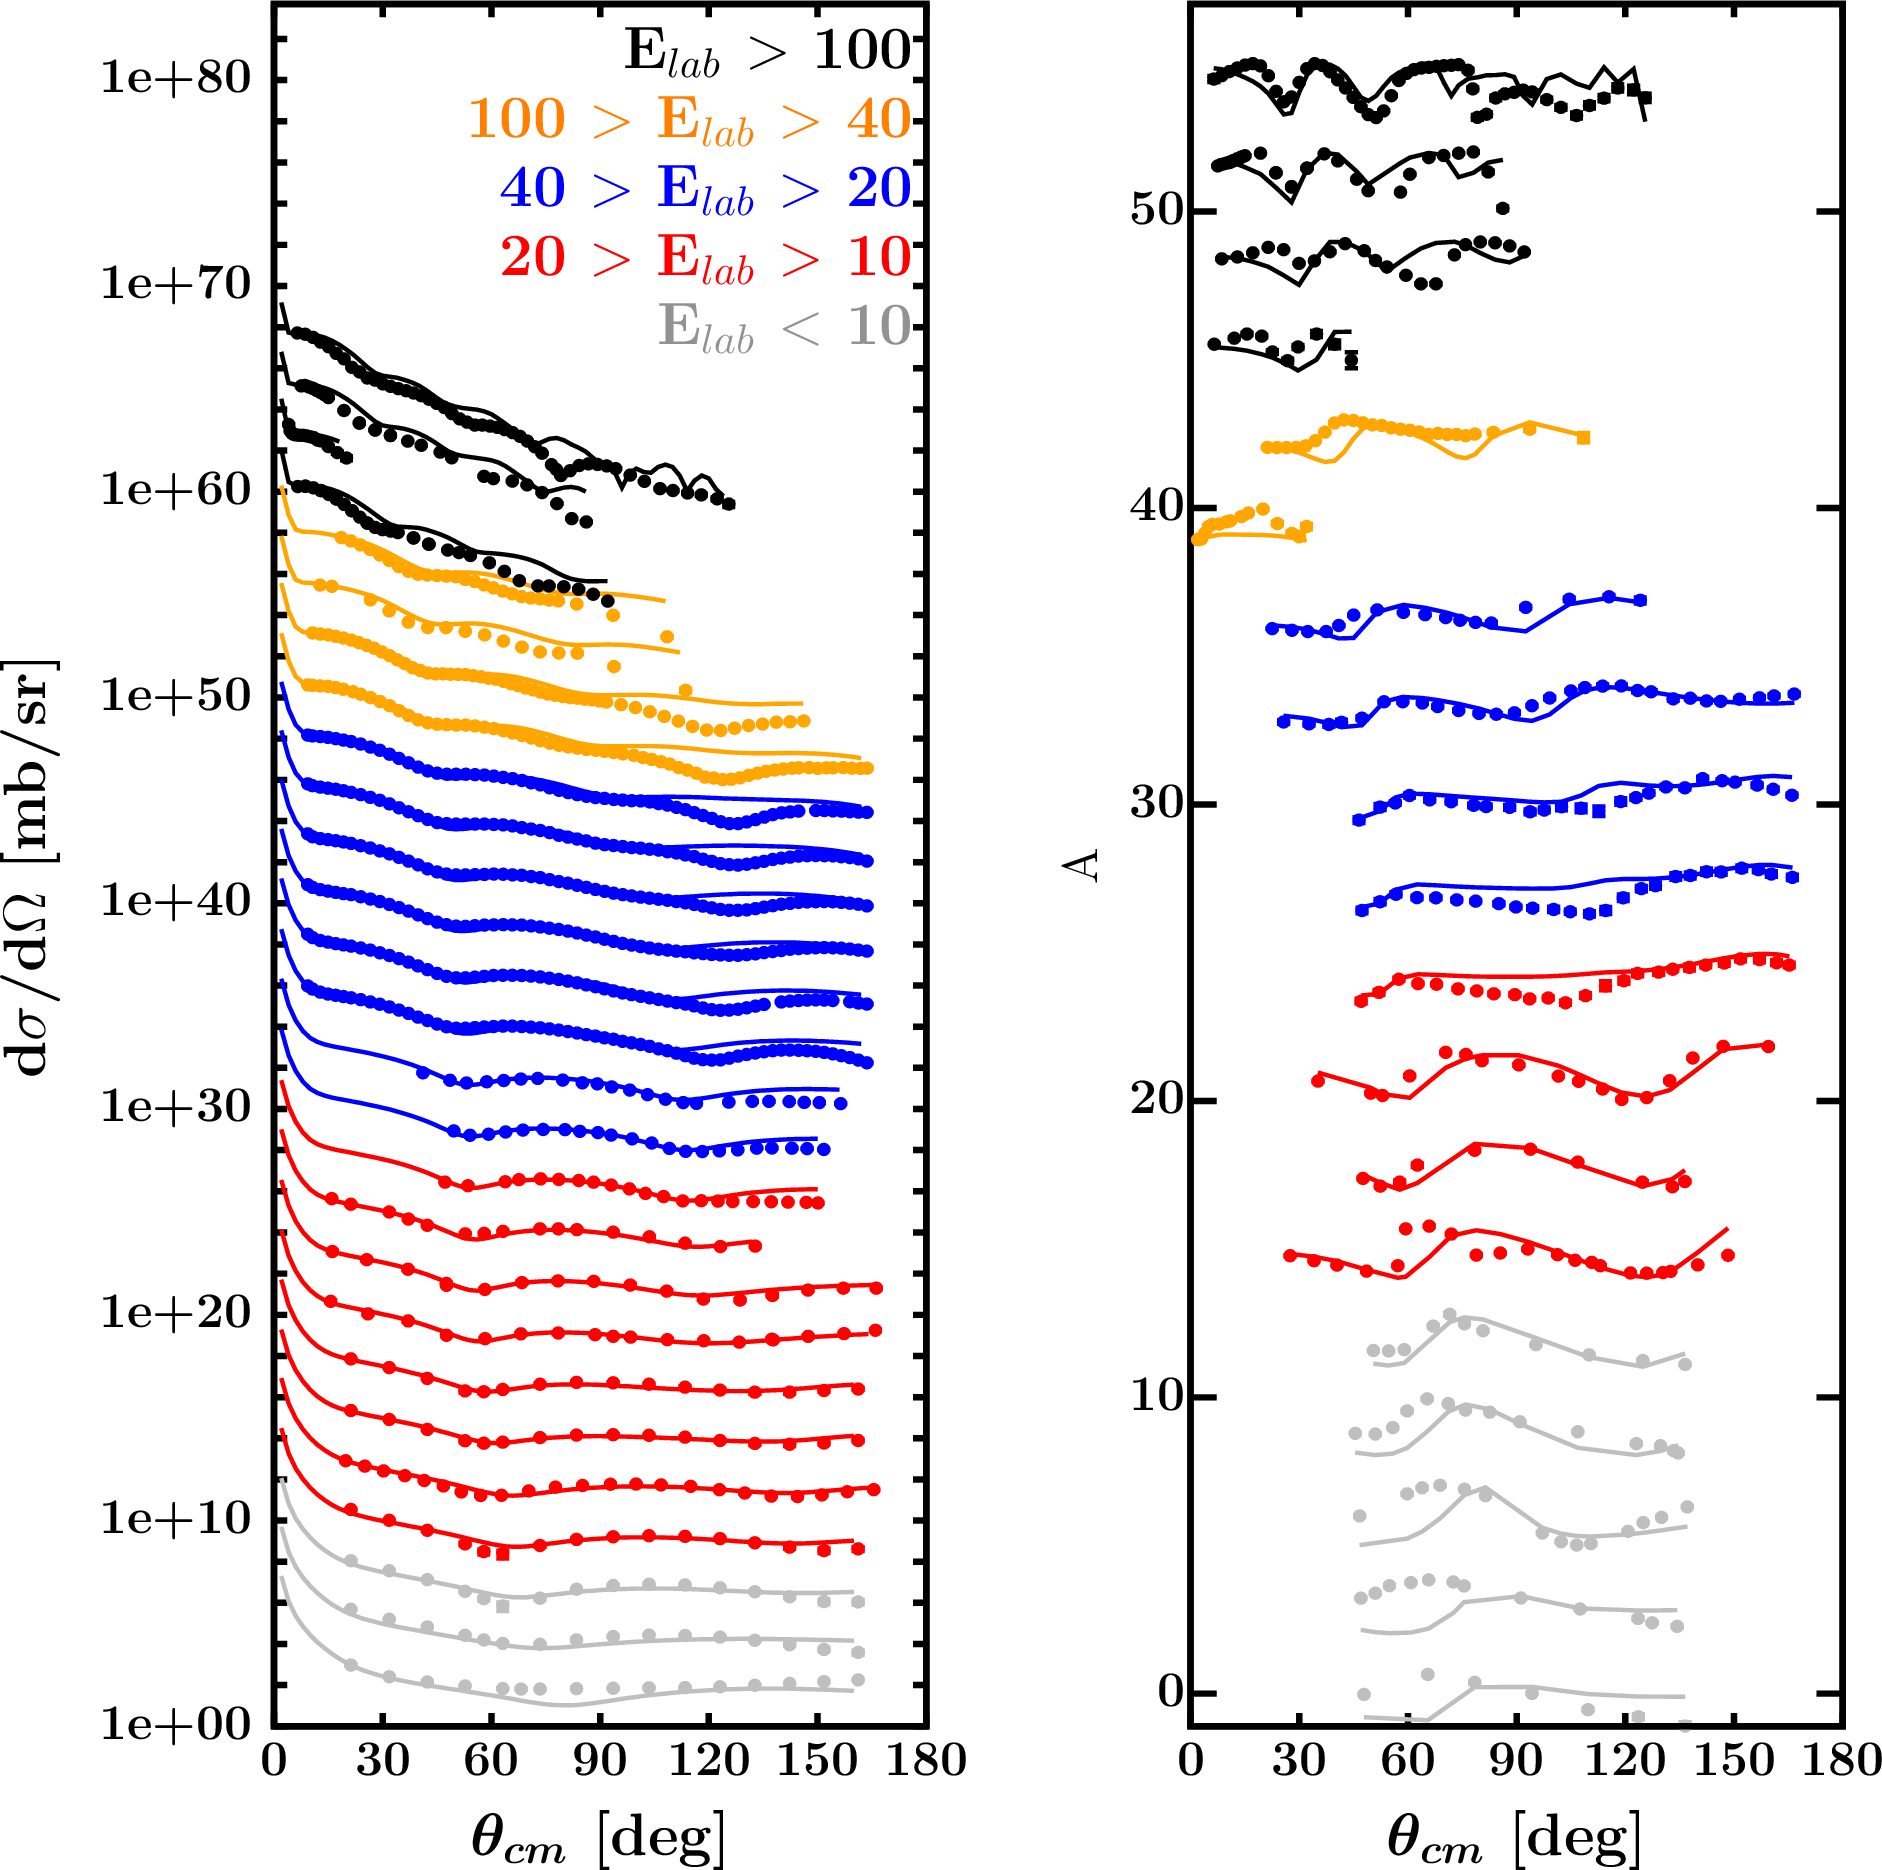
\includegraphics[width=1.0\textwidth]{figures/o16_protonElastic.png}
        \caption{Proton elastic scattering data}
        \label{DOMFitData_o16_proton_elastic}
    \end{minipage}\hfill
    \begin{minipage}{0.45\textwidth}
        \centering
        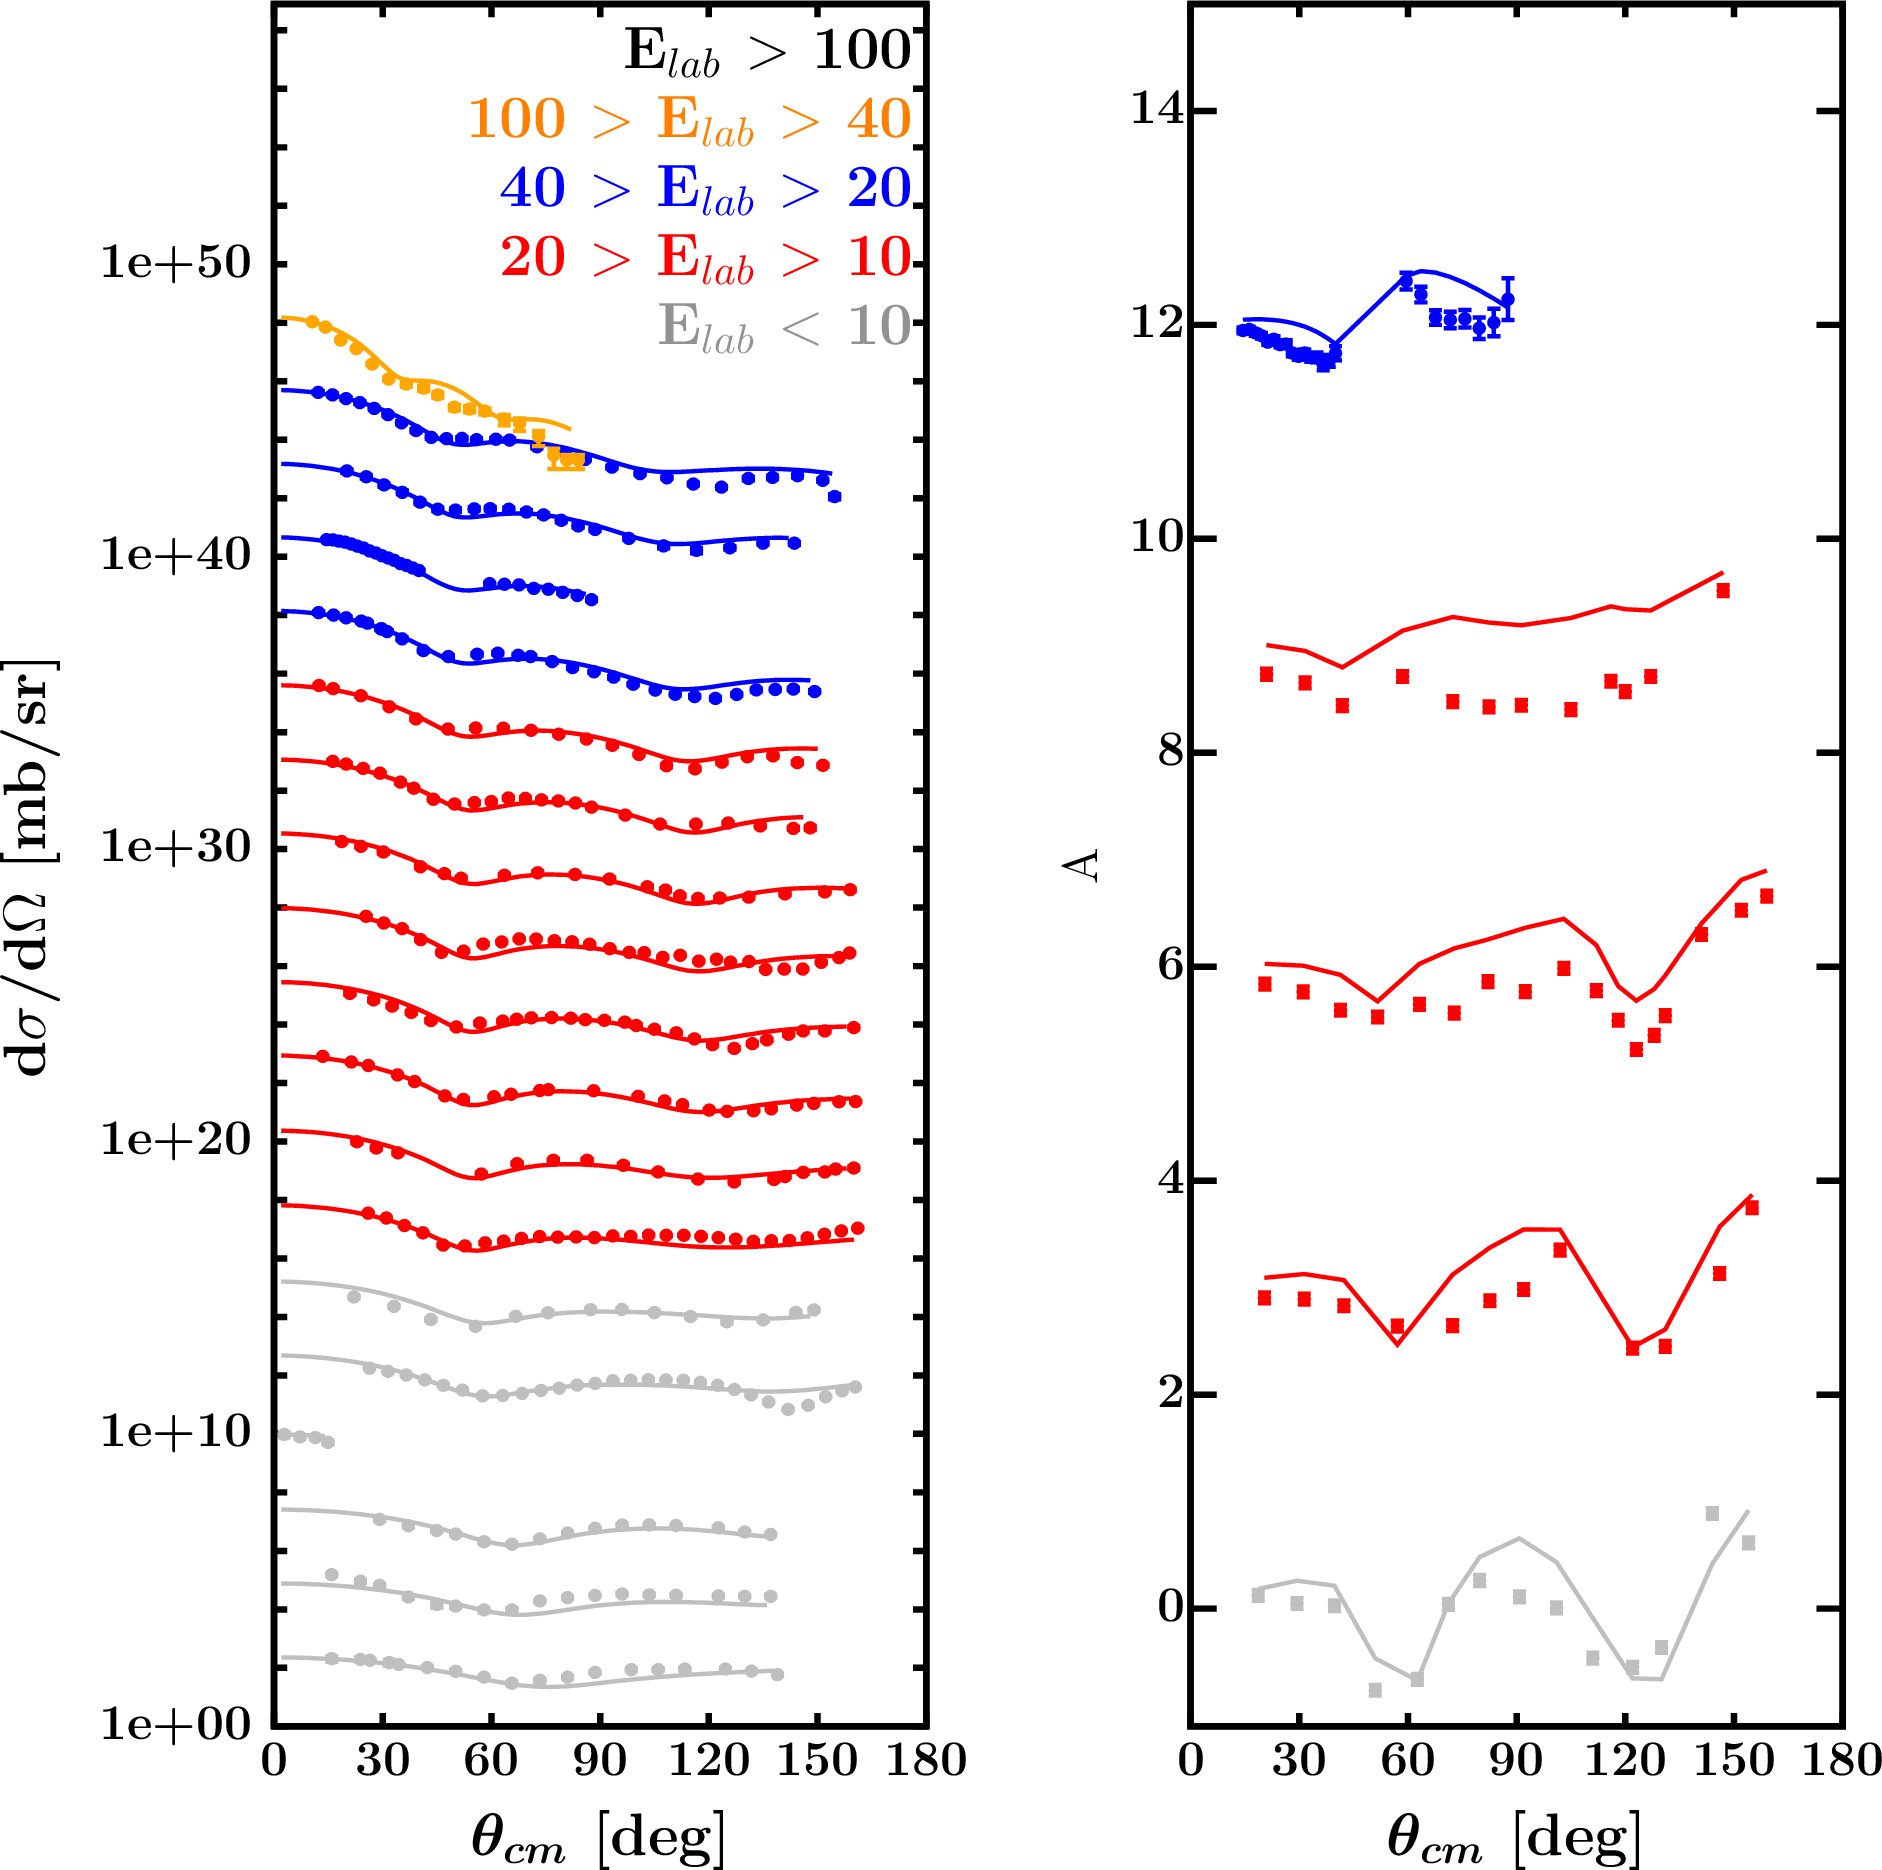
\includegraphics[width=1.0\textwidth]{figures/o16_neutronElastic.png}
        \caption{Neutron elastic scattering data}
        \label{DOMFitData_o16_neutron_elastic}
    \end{minipage}
\end{figure}

\begin{figure}[H]
    \centering
    \begin{minipage}{0.45\textwidth}
        \centering
        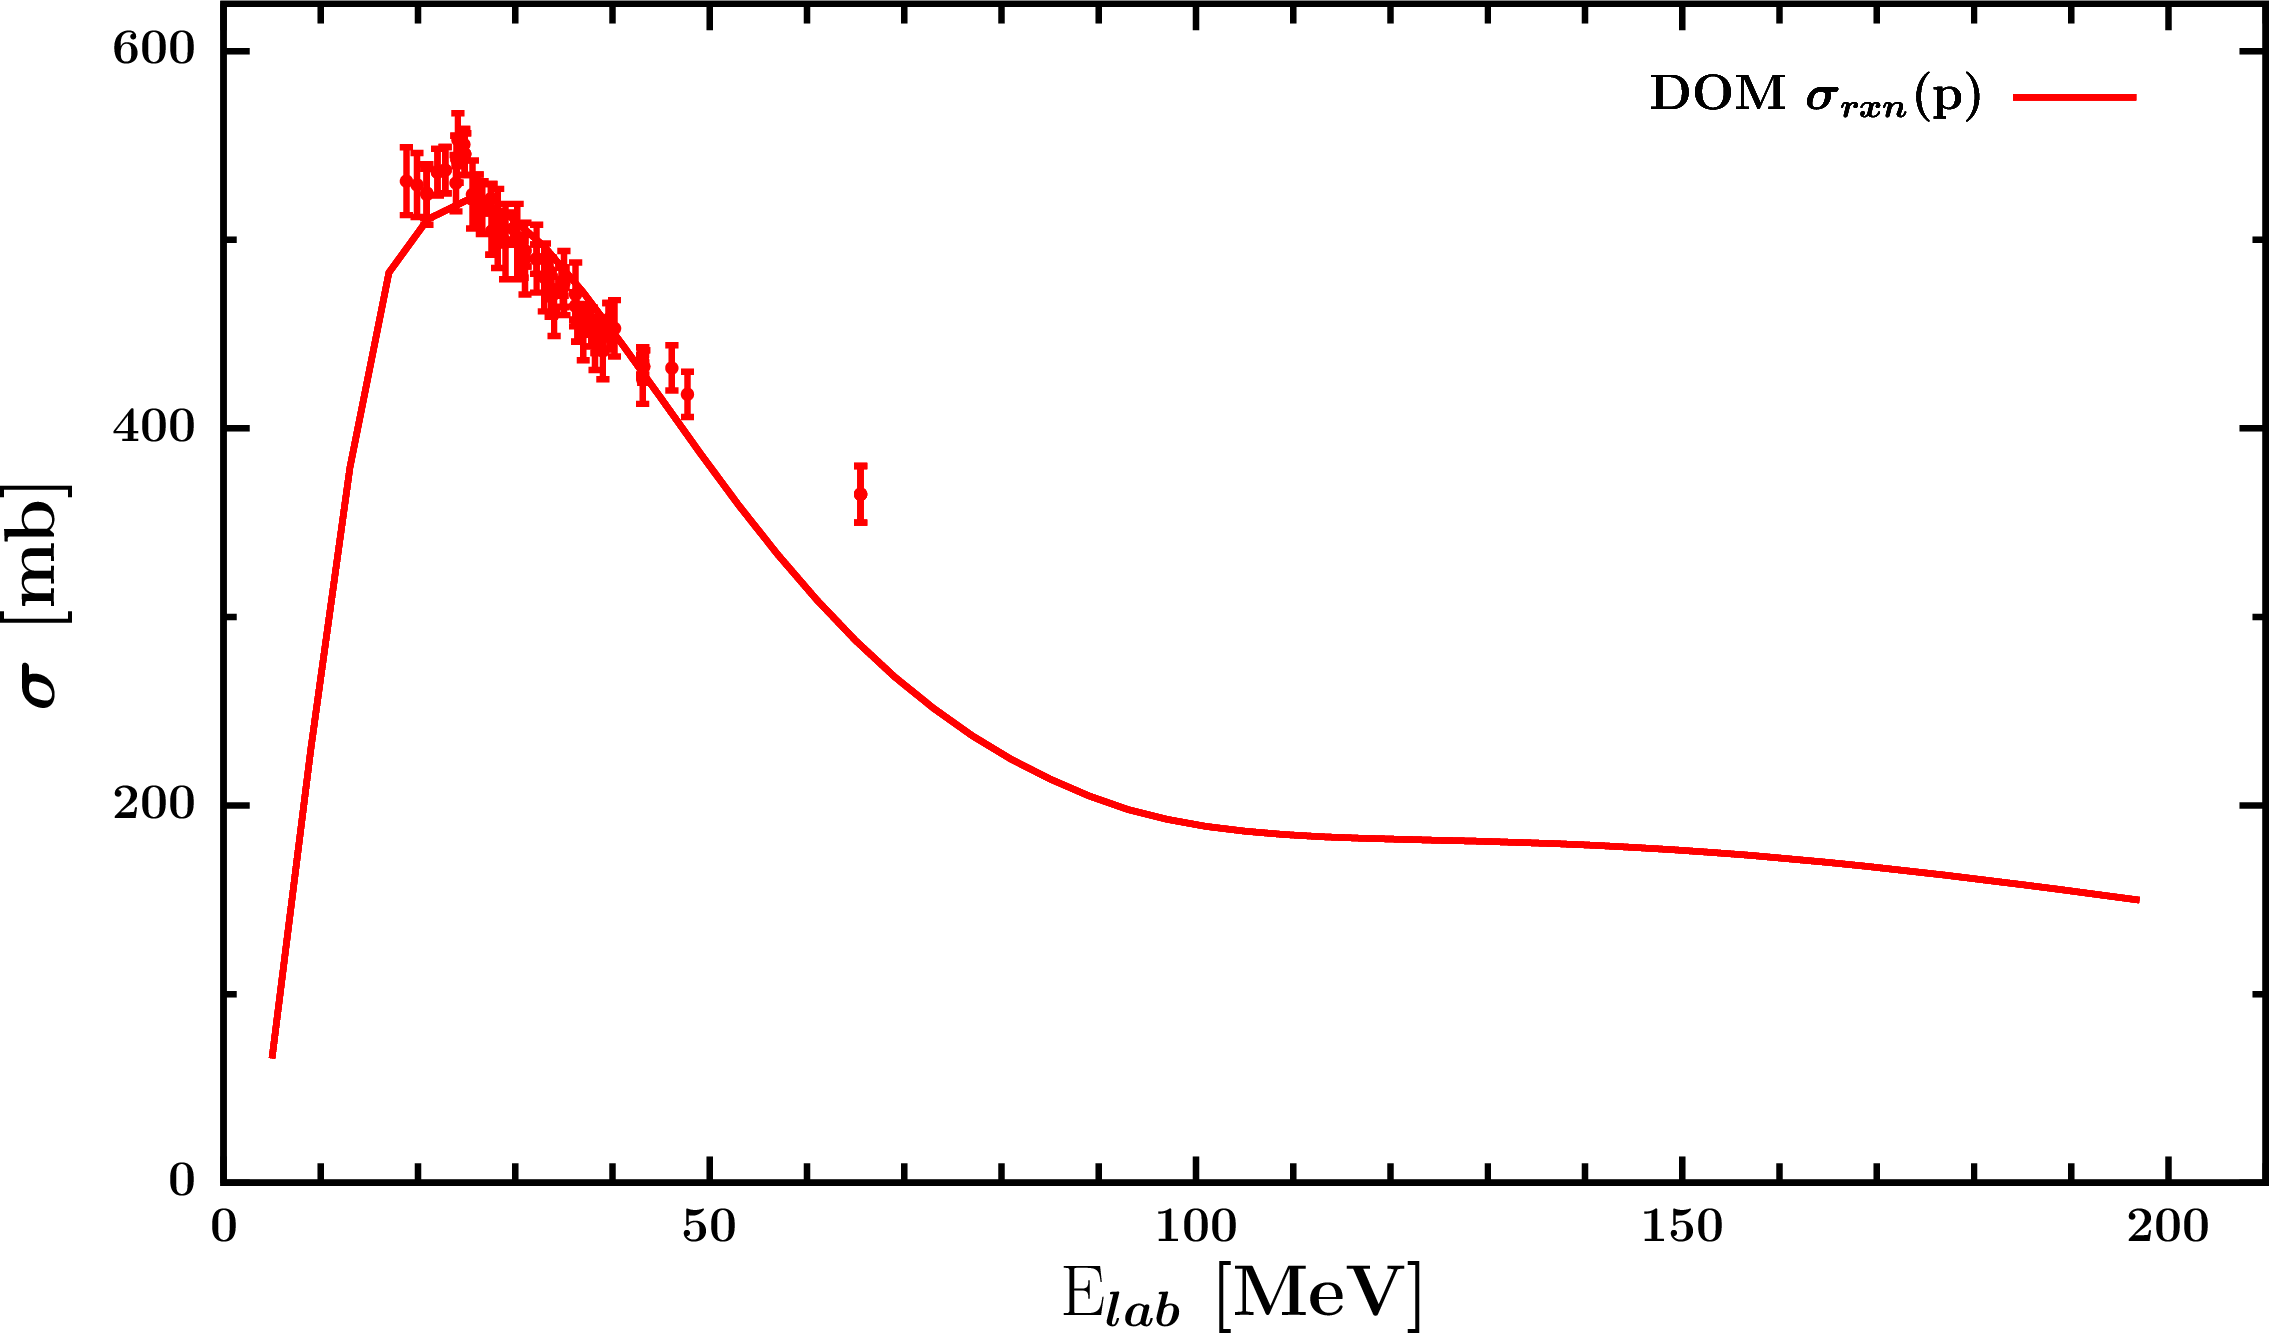
\includegraphics[width=1.0\textwidth]{figures/o16_protonInelastic.png}
        \caption{Proton \rxn data}
        \label{DOMFitData_o16_proton_inelastic}
    \end{minipage}\hfill
    \begin{minipage}{0.45\textwidth}
        \centering
        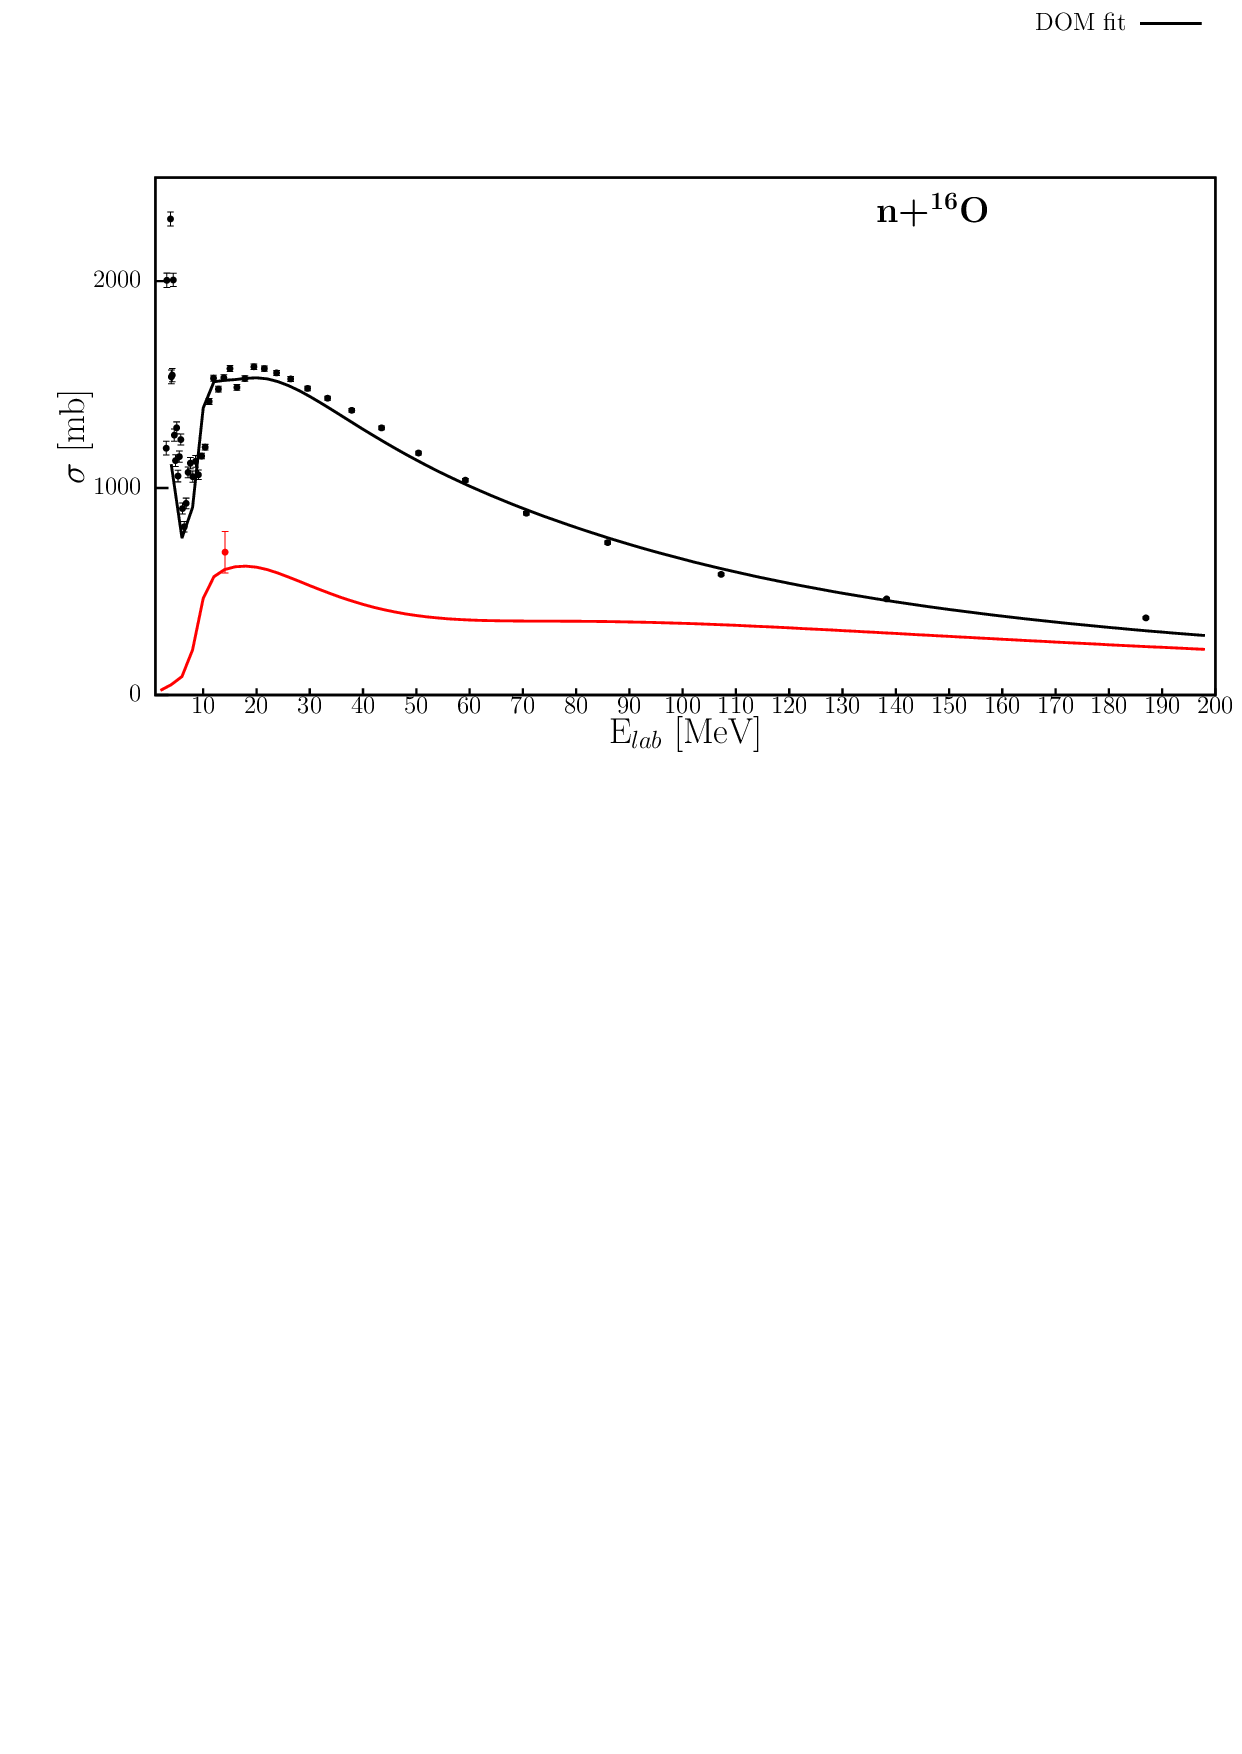
\includegraphics[width=1.0\textwidth]{figures/o16_neutronInelastic.png}
        \caption{Neutron \rxn and \tot data}
        \label{DOMFitData_o16_neutron_inelastic}
    \end{minipage}
\end{figure}

\afterpage{\clearpage}

\begin{figure}[H]
    \centering
    \begin{minipage}{0.45\textwidth}
        \centering
        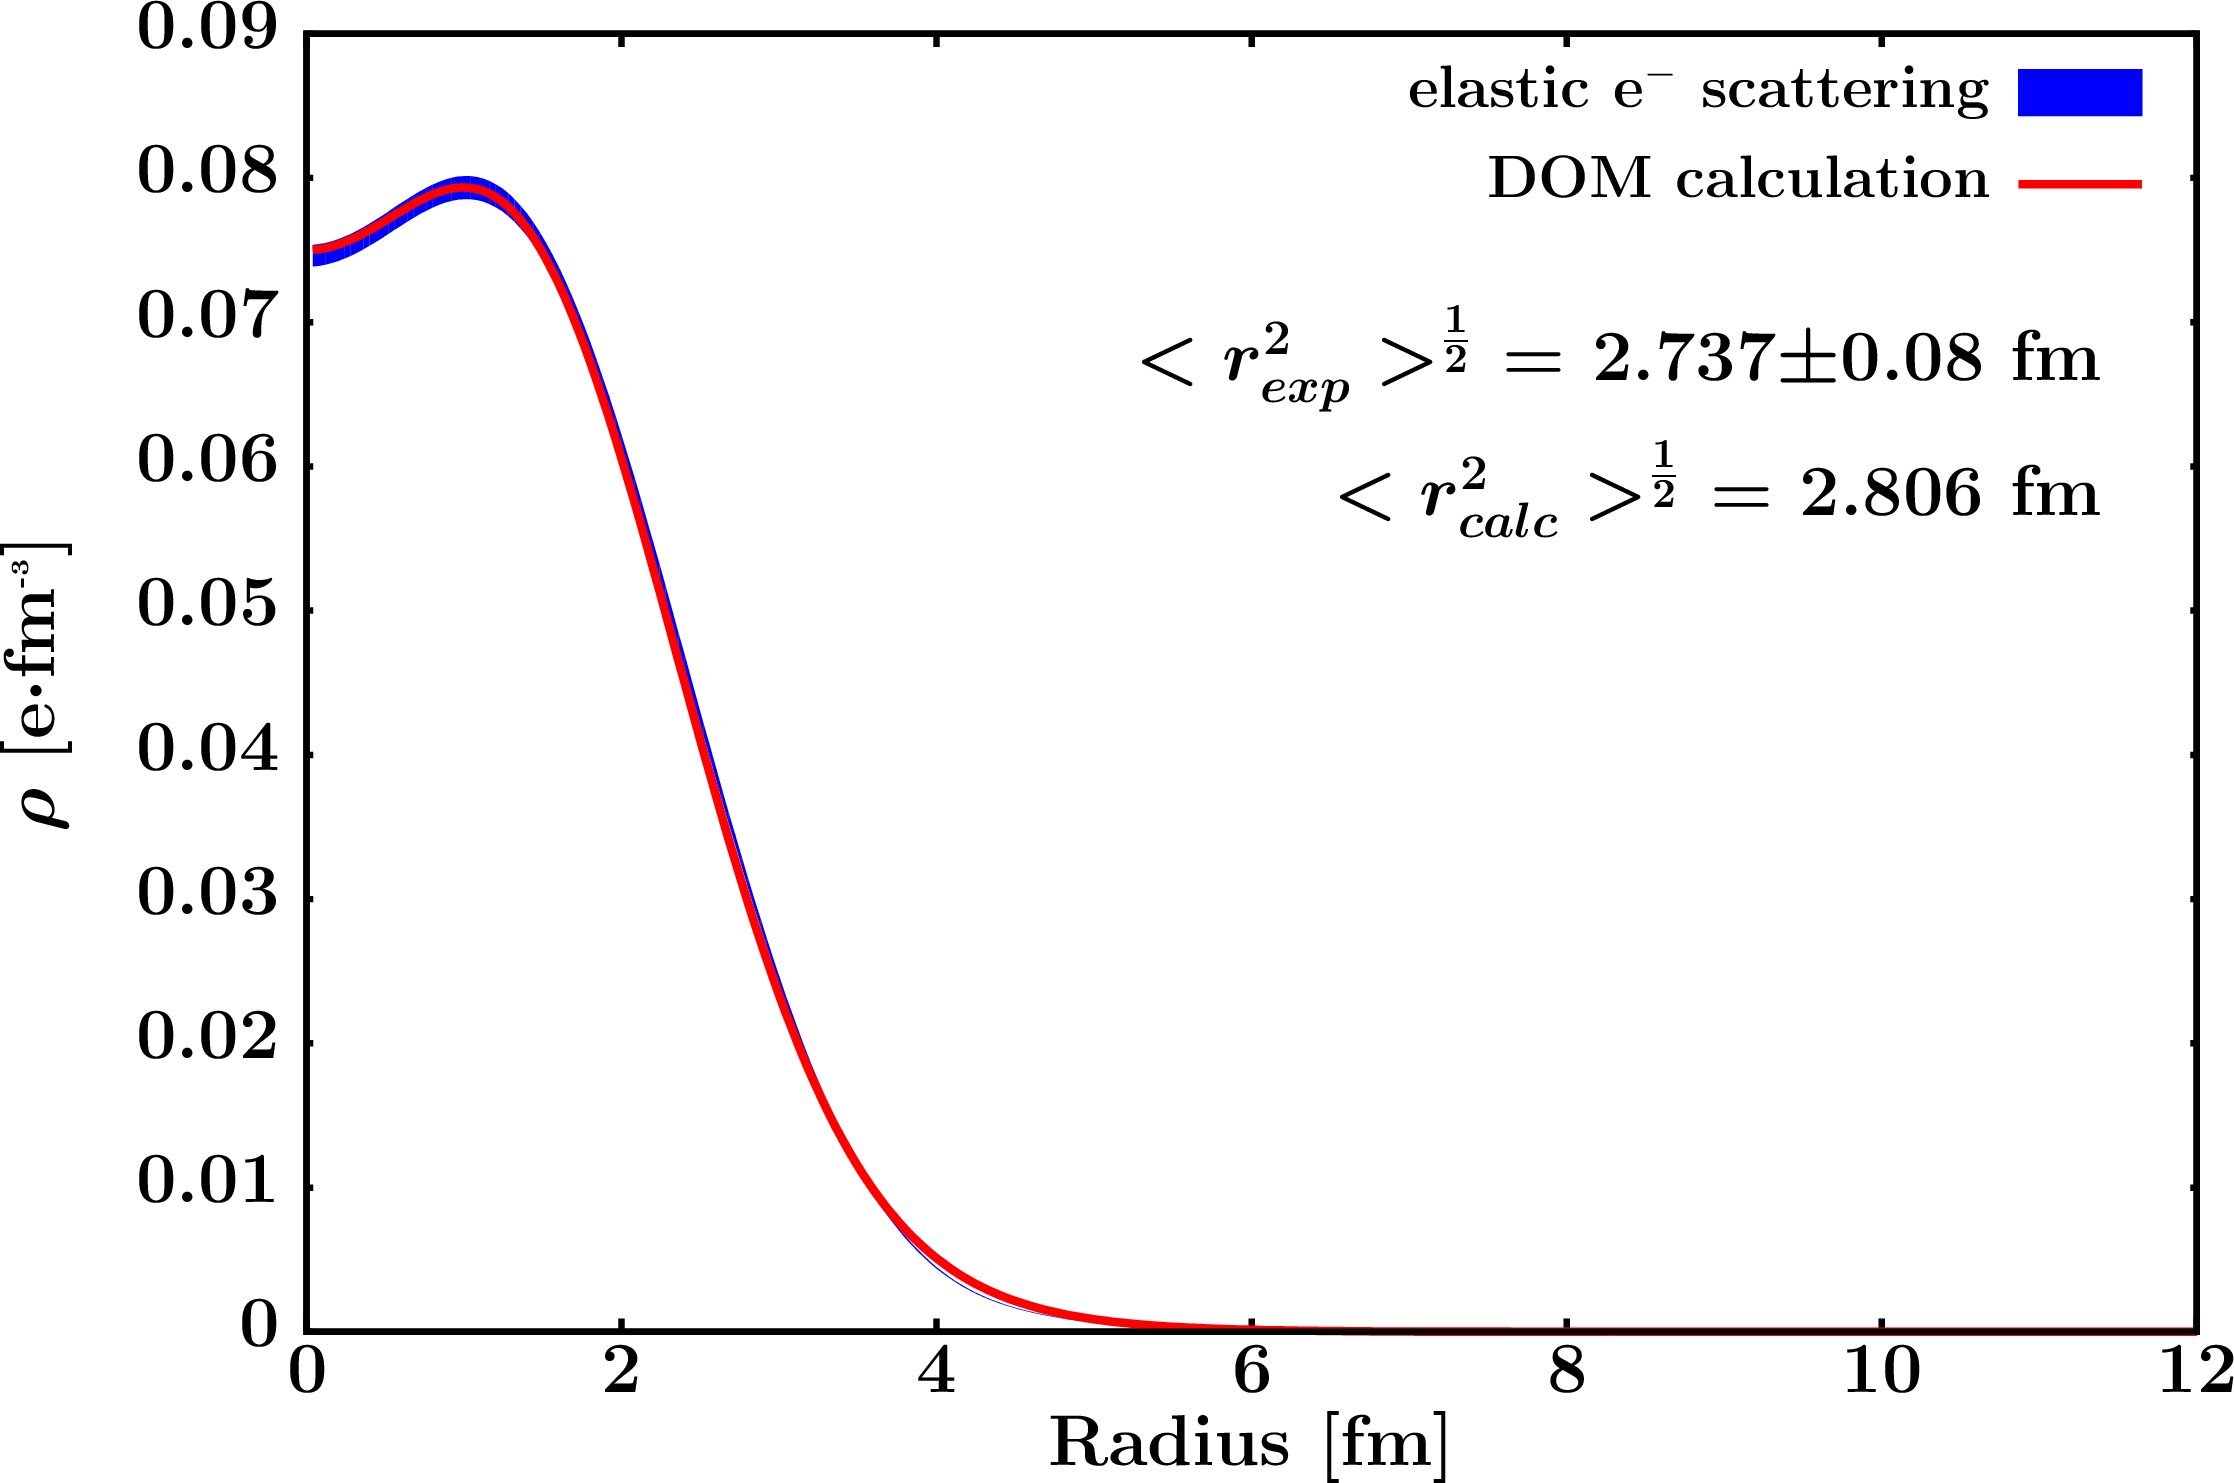
\includegraphics[width=1.0\textwidth]{figures/o16_chargeDensity.png}
        \caption{Charge density data}
        \label{DOMFitData_o16_chargeDensity}
    \end{minipage}\hfill
    \begin{minipage}{0.45\textwidth}
        \centering
        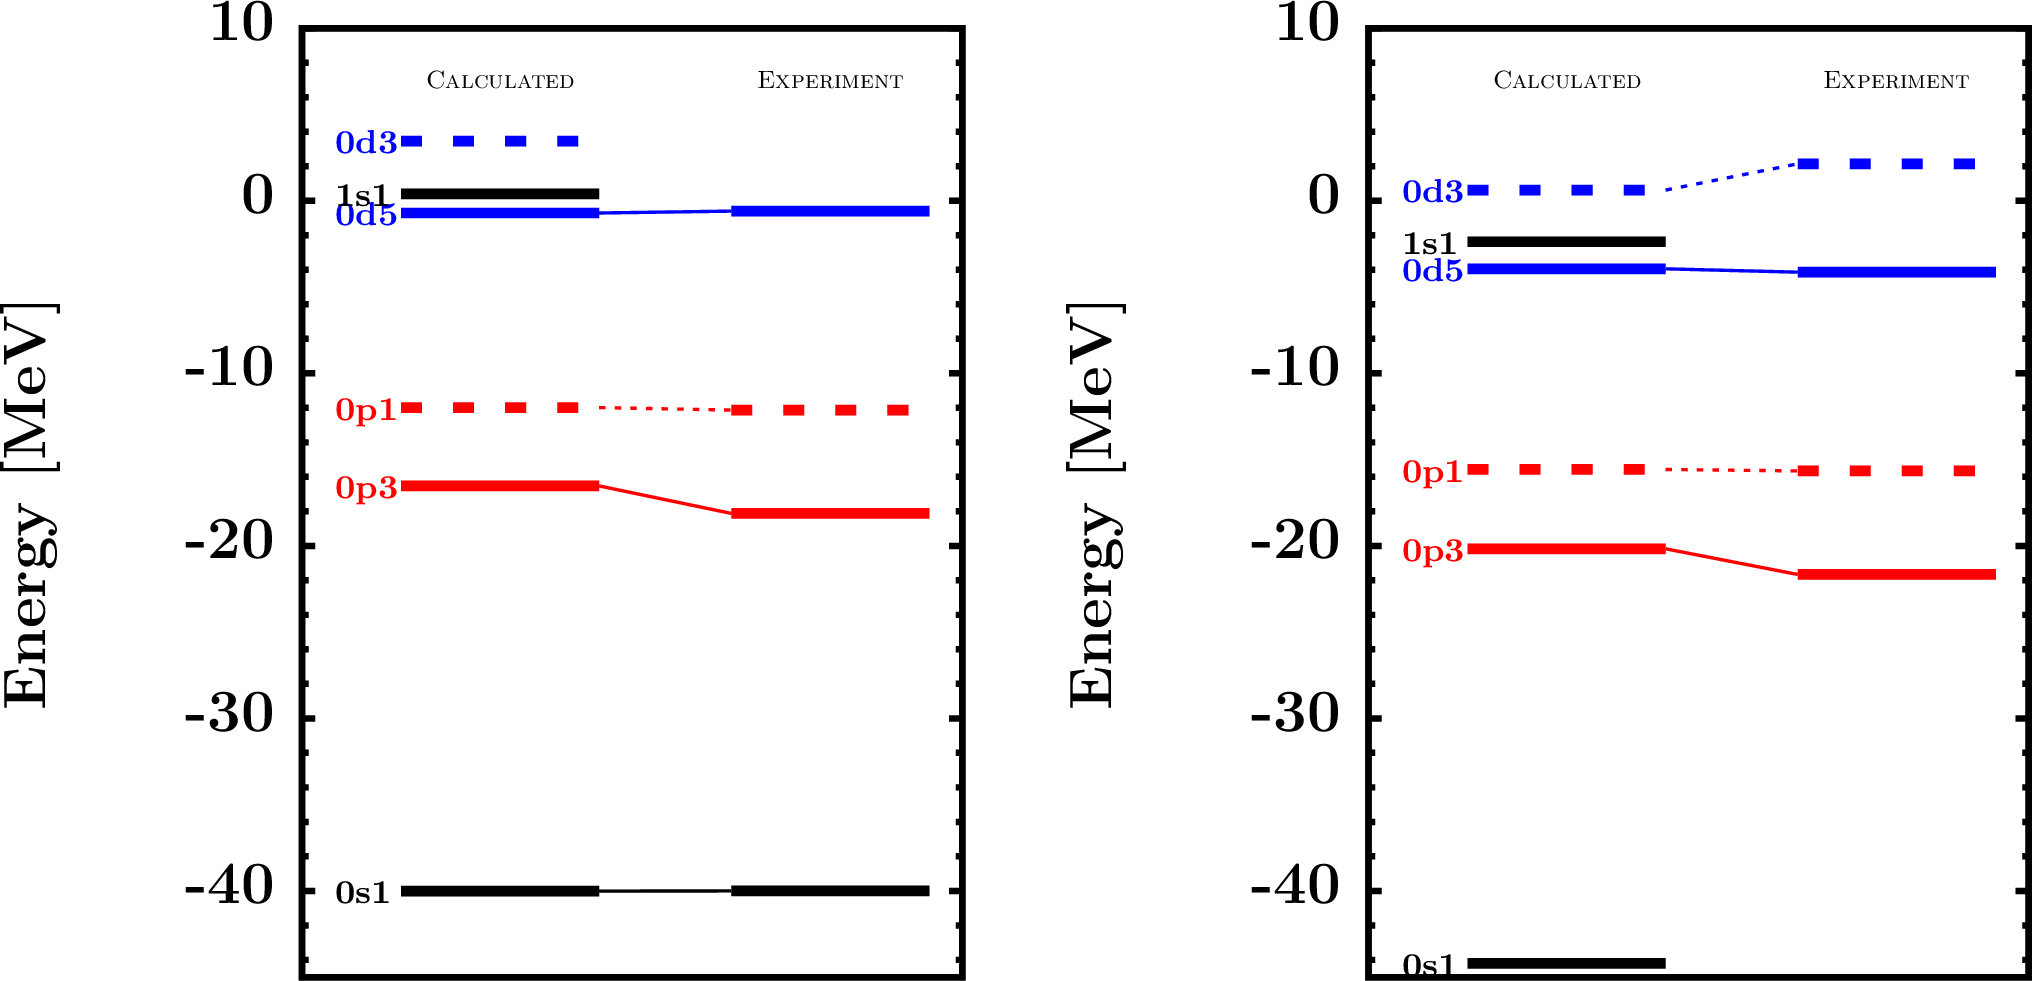
\includegraphics[width=1.0\textwidth]{figures/o16_SPLevels.png}
        \caption{Single-particle levels}
        \label{DOMFitData_o16_SPLevels}
    \end{minipage}
\end{figure}

\afterpage{\clearpage}

\begin{figure}[H]
    \centering
    \begin{minipage}{0.45\textwidth}
        \centering
        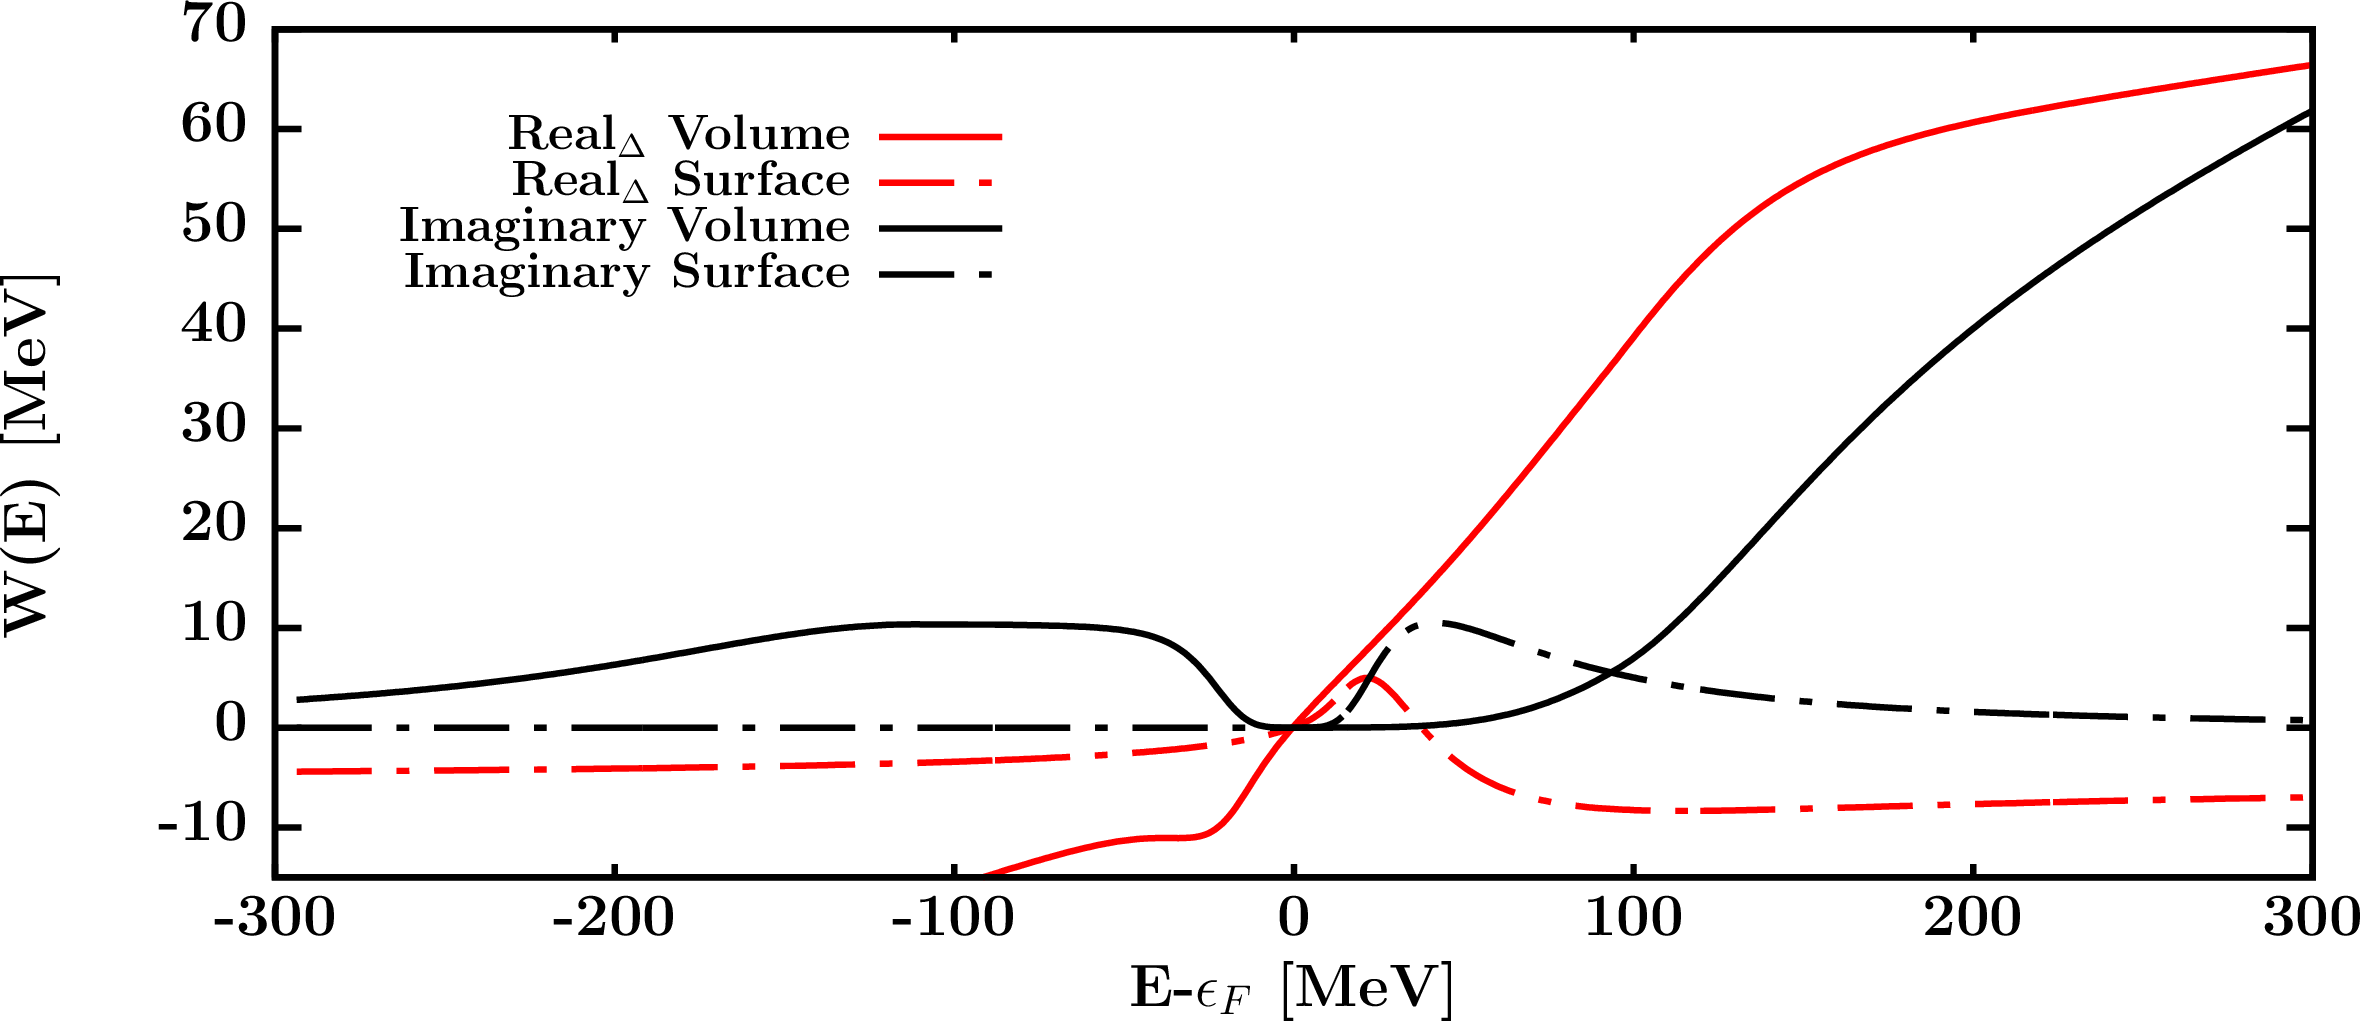
\includegraphics[width=1.0\textwidth]{figures/o16_protonPotentials.png}
        \caption{Energy-dependence of optical potential components for protons
        on \oSix}
        \label{DOMFitData_o16_proton_potentialComponent_energy}
    \end{minipage}\hfill
    \begin{minipage}{0.45\textwidth}
        \centering
        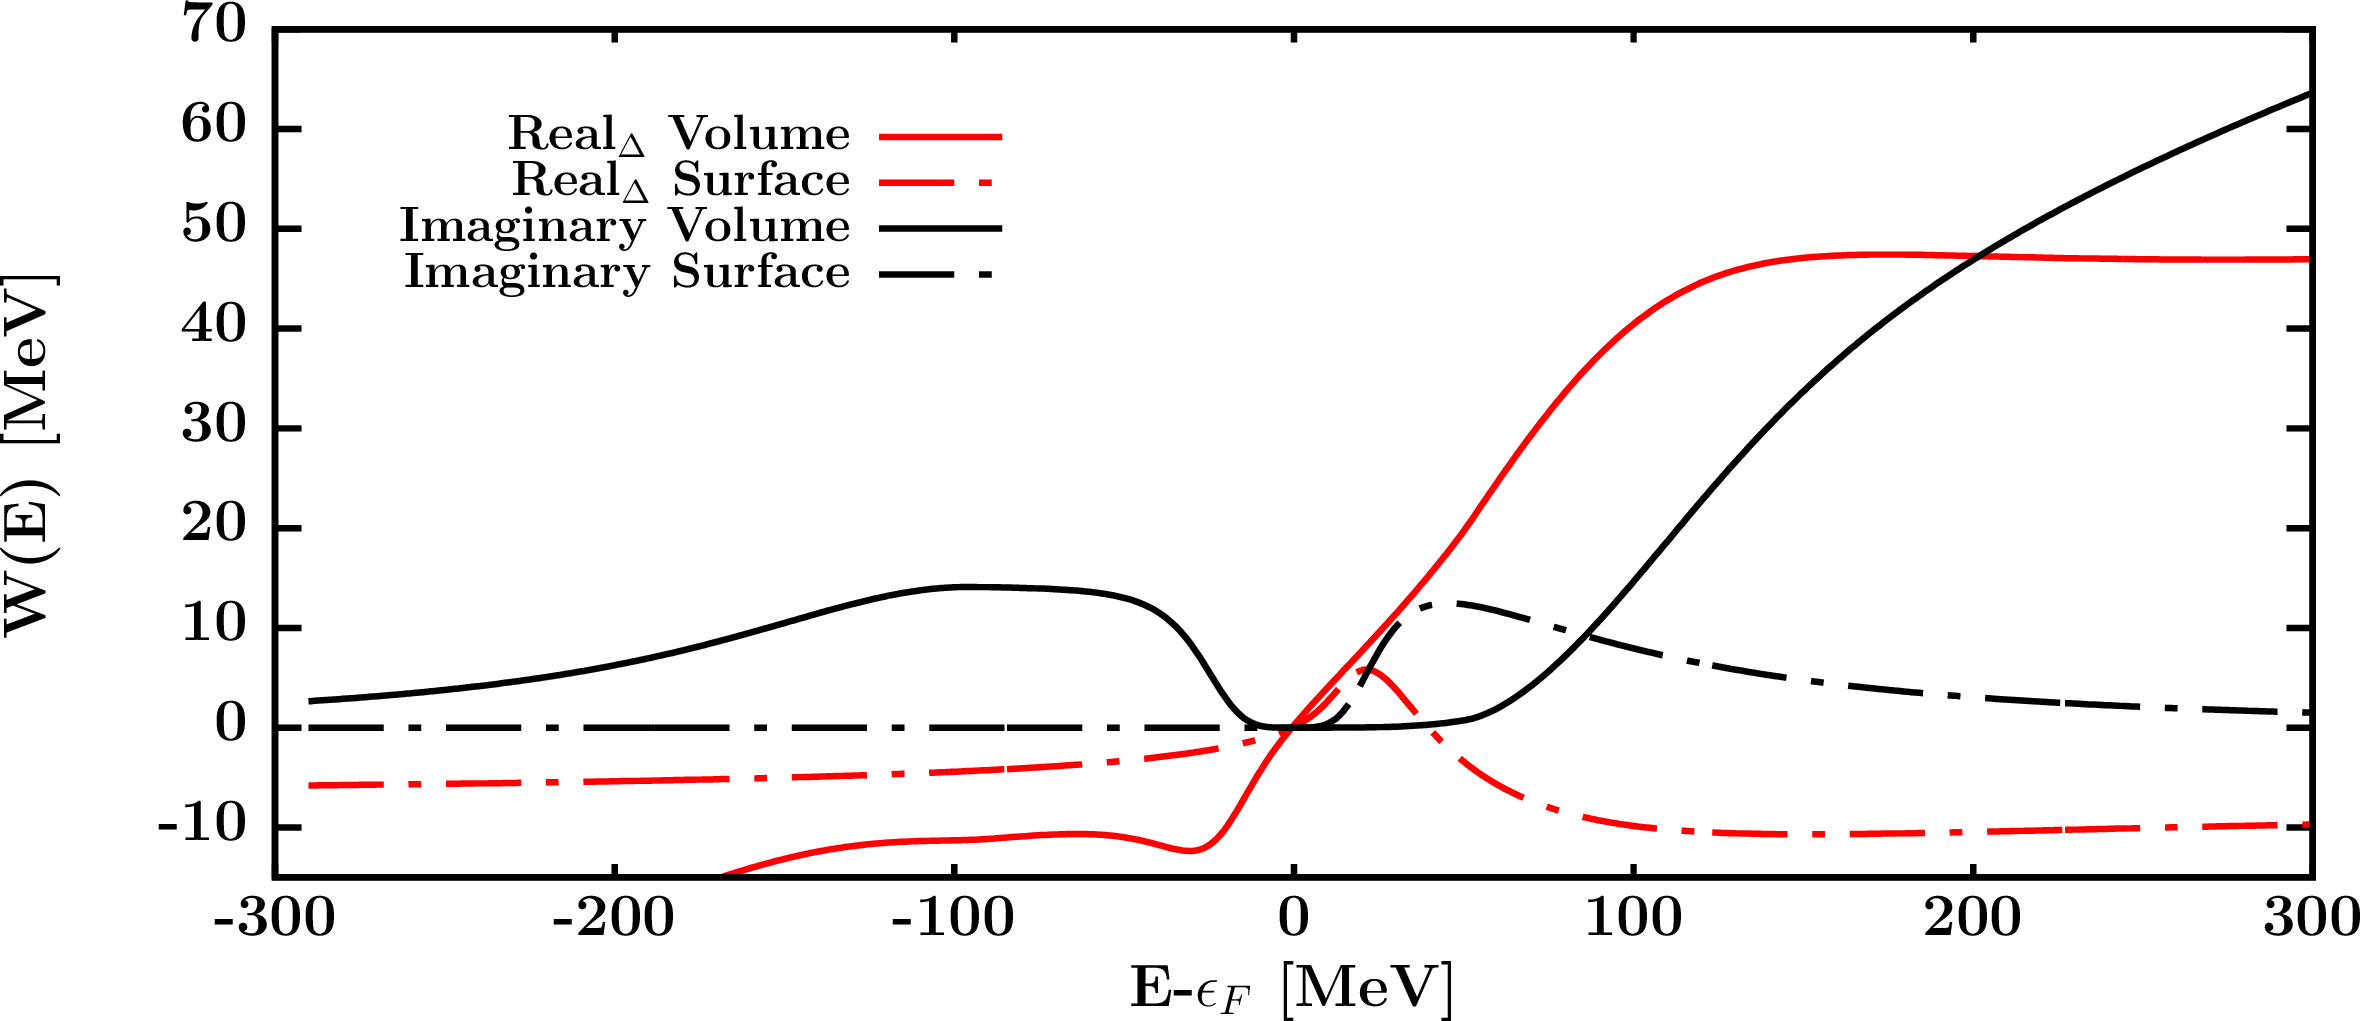
\includegraphics[width=1.0\textwidth]{figures/o16_neutronPotentials.png}
        \caption{Neutron potential energy-dependent component}
        \label{DOMFitData_o16_neutron_potentialComponent_energy}
    \end{minipage}
\end{figure}

\begin{figure}[H]
    \centering
    \begin{minipage}{0.45\textwidth}
        \centering
        
\includegraphics[width=1.0\textwidth]{figures/o16_protonVolumeIntegrals.png}
        \caption{Proton potential, integrated over r-space}
        \label{DOMFitData_o16_proton_potentialIntegral}
    \end{minipage}\hfill
    \begin{minipage}{0.45\textwidth}
        \centering
        
\includegraphics[width=1.0\textwidth]{figures/o16_neutronVolumeIntegrals.png}
        \caption{Neutron potential, integrated over r-space}
        \label{DOMFitData_o16_neutron_potentialIntegral}
    \end{minipage}
\end{figure}

\afterpage{\clearpage}

\begin{figure}[H]
    \centering
    \begin{minipage}{0.45\textwidth}
        \centering
        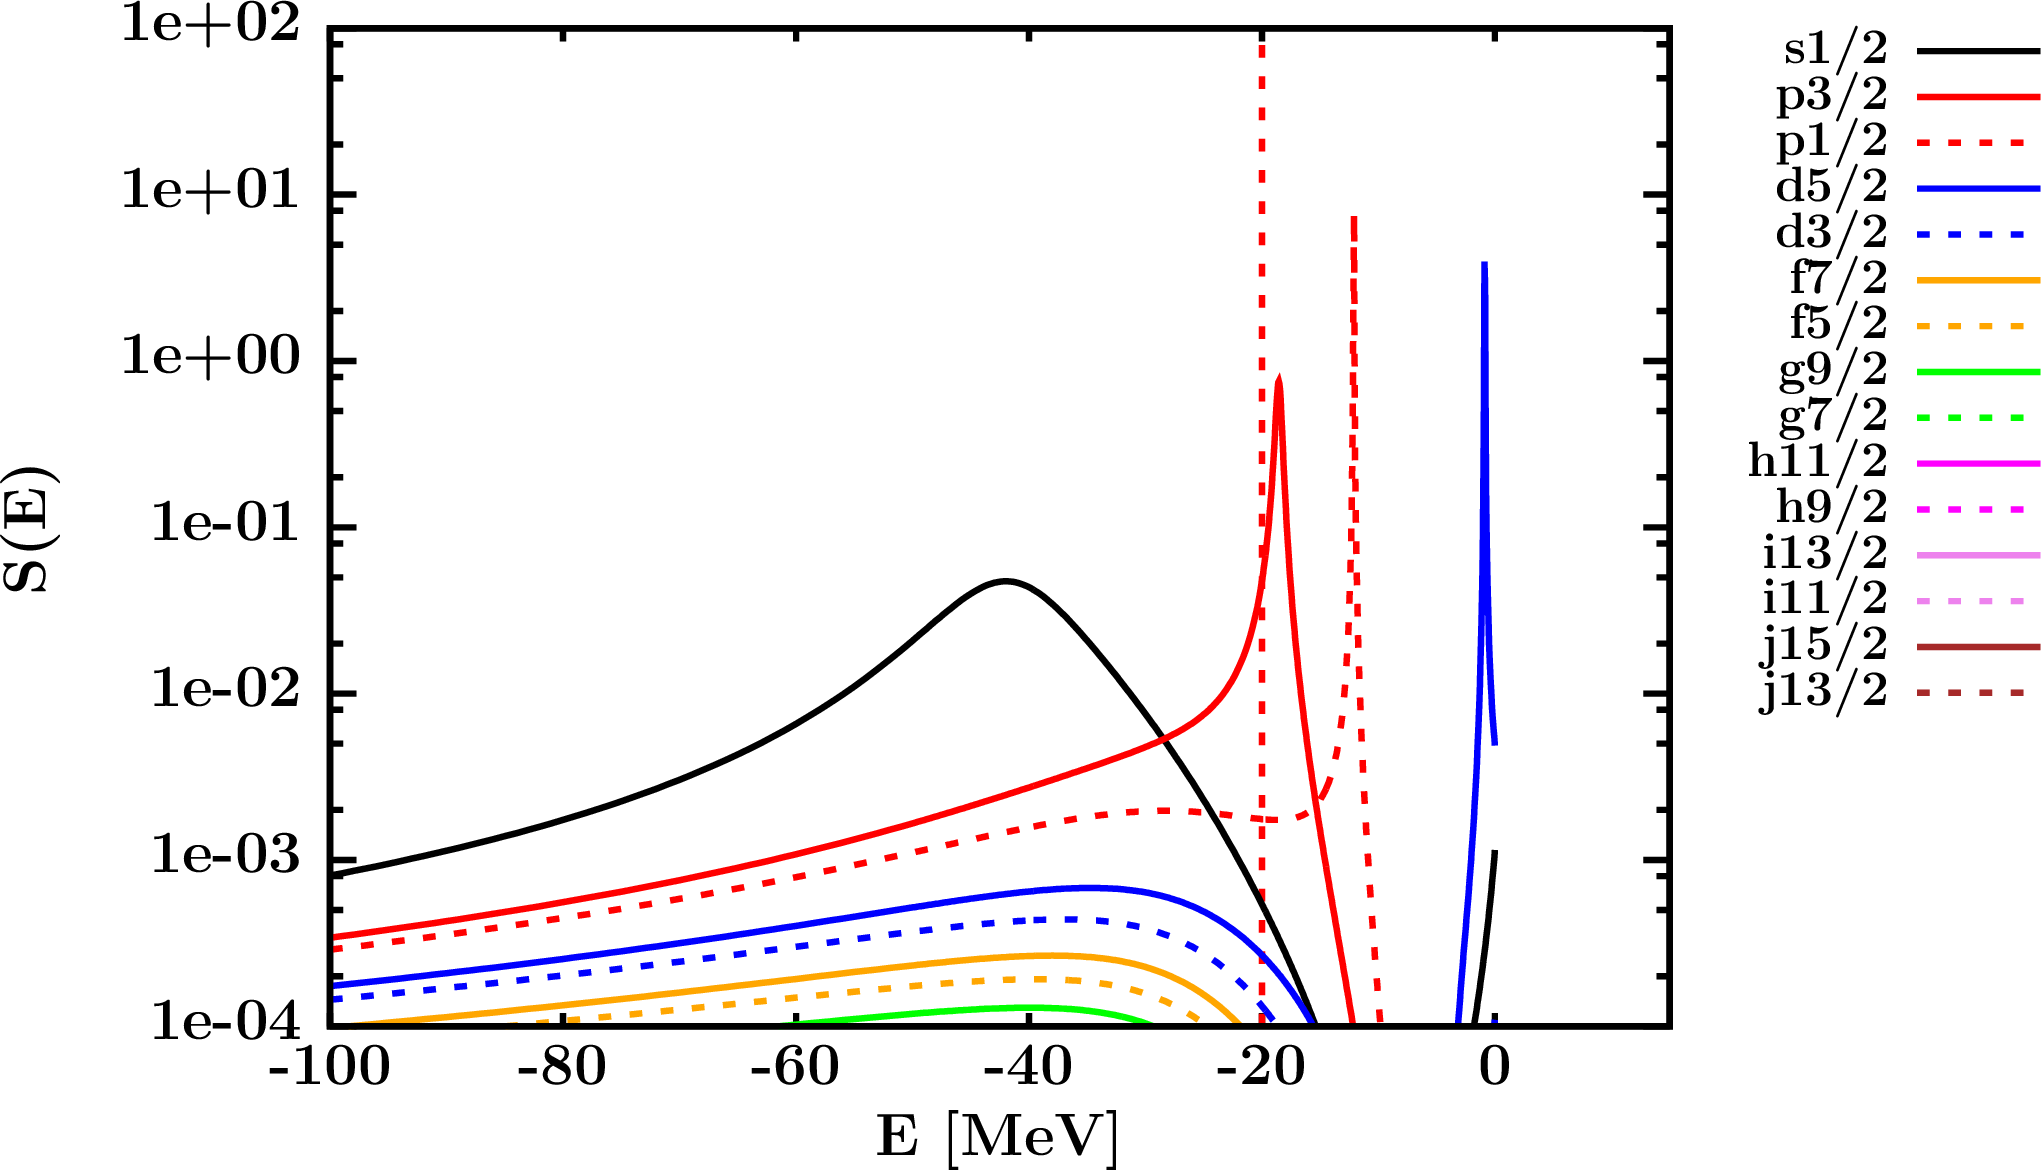
\includegraphics[width=1.0\textwidth]{figures/o16_protonSpectralFunctions.png}
        \caption{Proton spectral functions}
        \label{DOMFitData_o16_proton_spectralFunctions}
    \end{minipage}\hfill
    \begin{minipage}{0.45\textwidth}
        \centering
        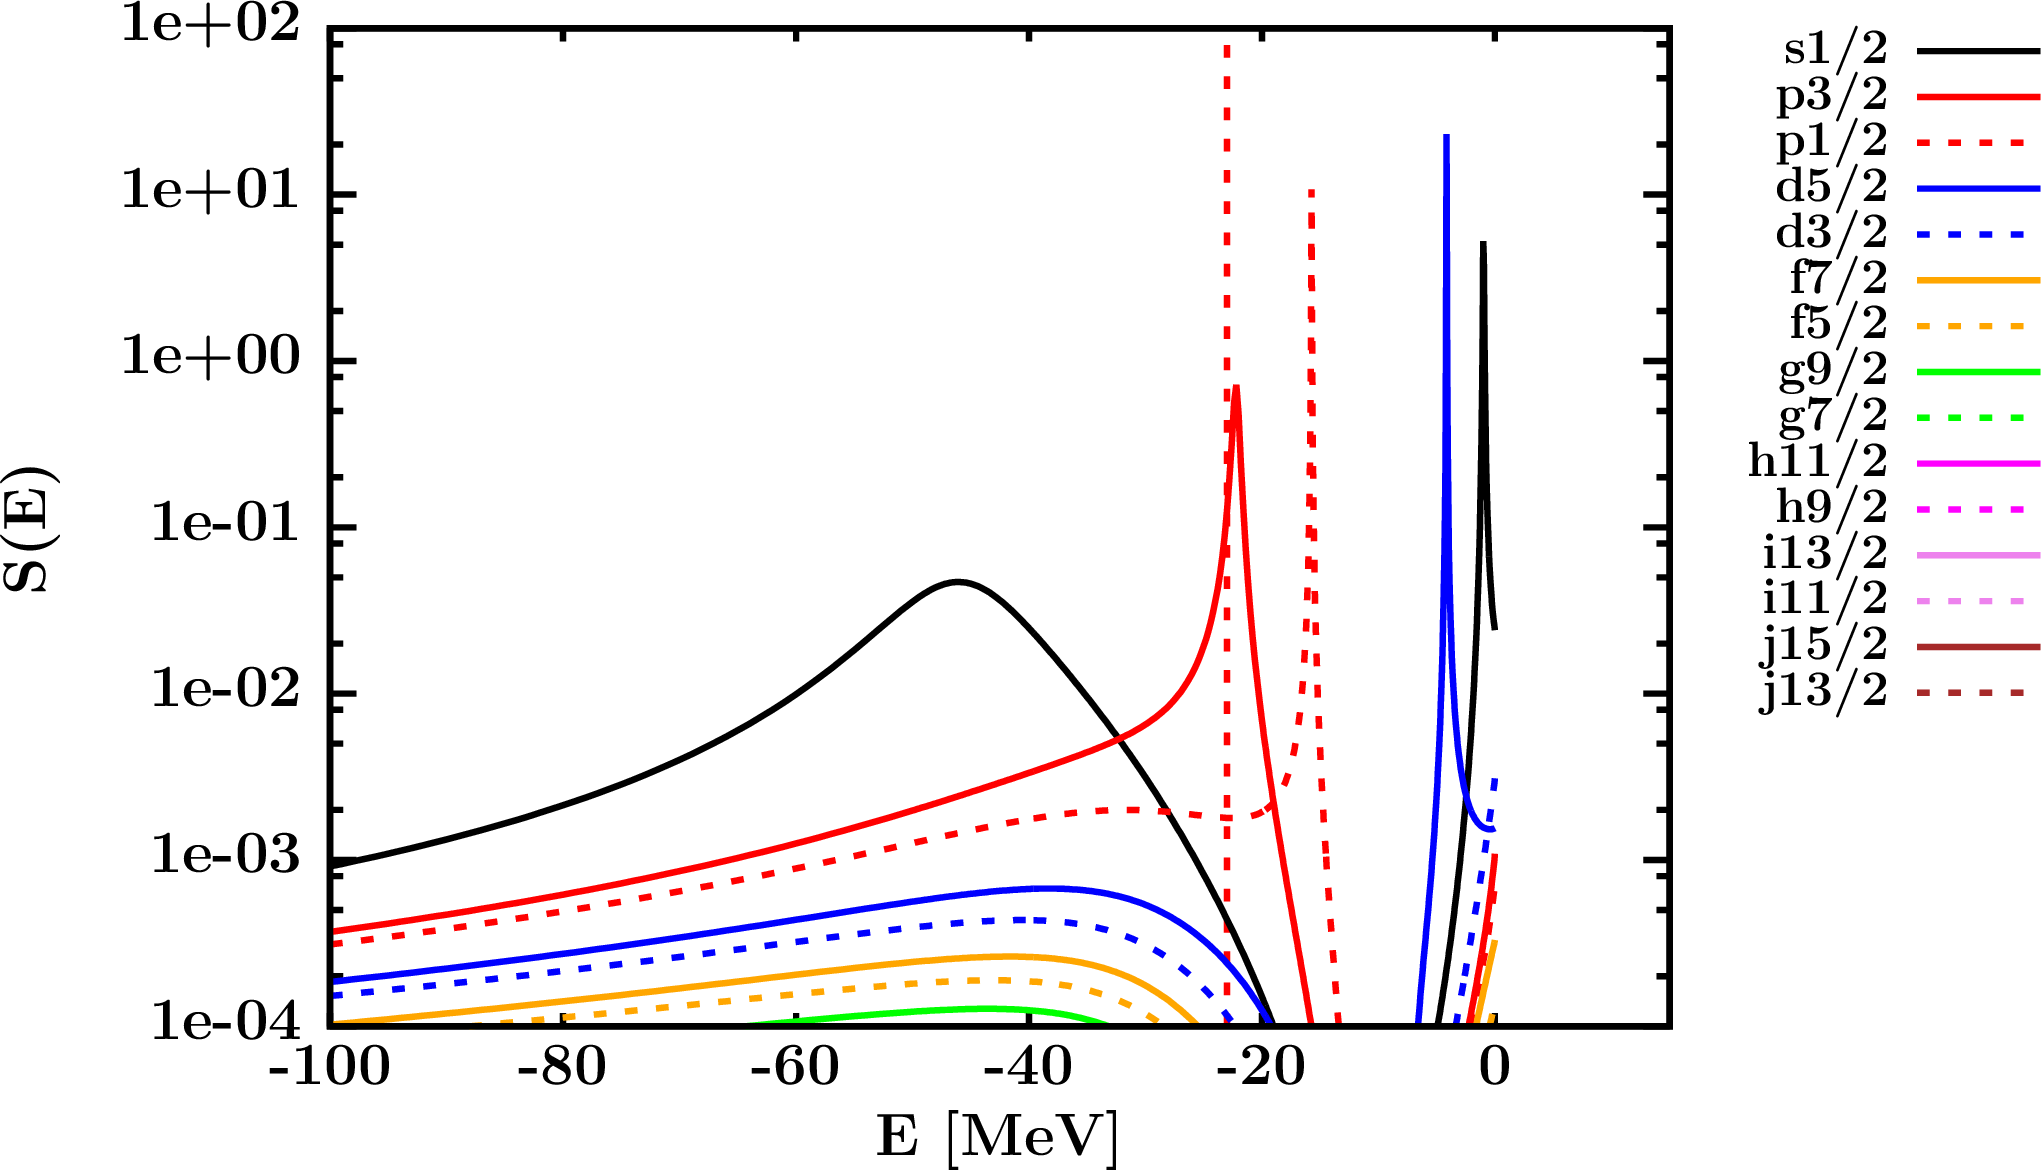
\includegraphics[width=1.0\textwidth]{figures/o16_neutronSpectralFunctions.png}
        \caption{Neutron spectral functions}
        \label{DOMFitData_o16_neutron_spectralFunctions}
    \end{minipage}
\end{figure}

\begin{figure}[H]
    \centering
    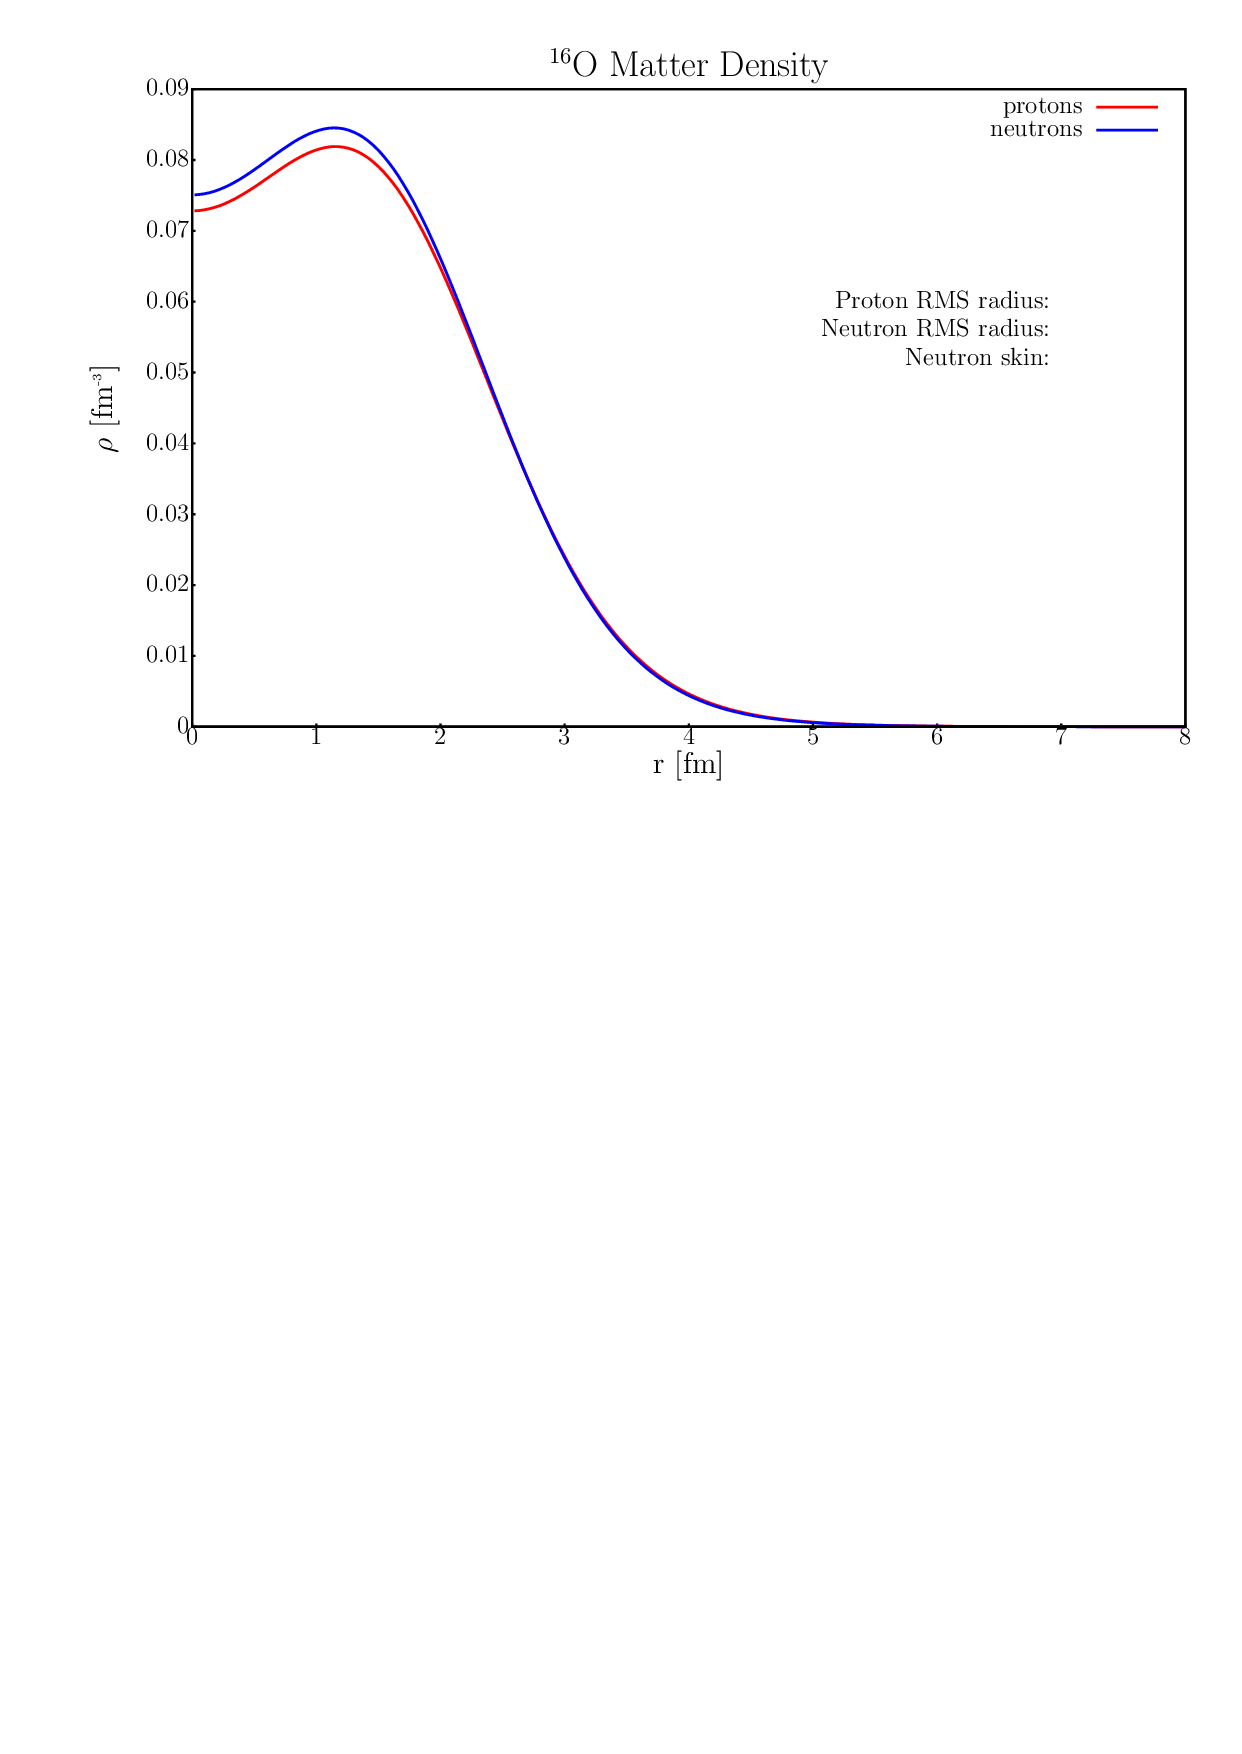
\includegraphics[width = 0.5\textwidth]{figures/o16_matterDensity.png}
    \caption{Matter density distribution}
    \label{DOMFitData_o16_matterDensity}
\end{figure}

\begin{figure}[H]
    \centering
    \includegraphics[width = 0.5\textwidth]{figures/o16_momentumDistribution.png}
    \caption{Momentum distribution}
    \label{DOMFitData_o16_momentumDistribution}
\end{figure}

\begin{figure}[H]
    \centering
    \includegraphics[width = 0.5\textwidth]{figures/o16_energyDensity.png}
    \caption{Energy density distribution}
    \label{DOMFitData_o16_energyDensity}
\end{figure}

\begin{figure}[H]
    \centering
    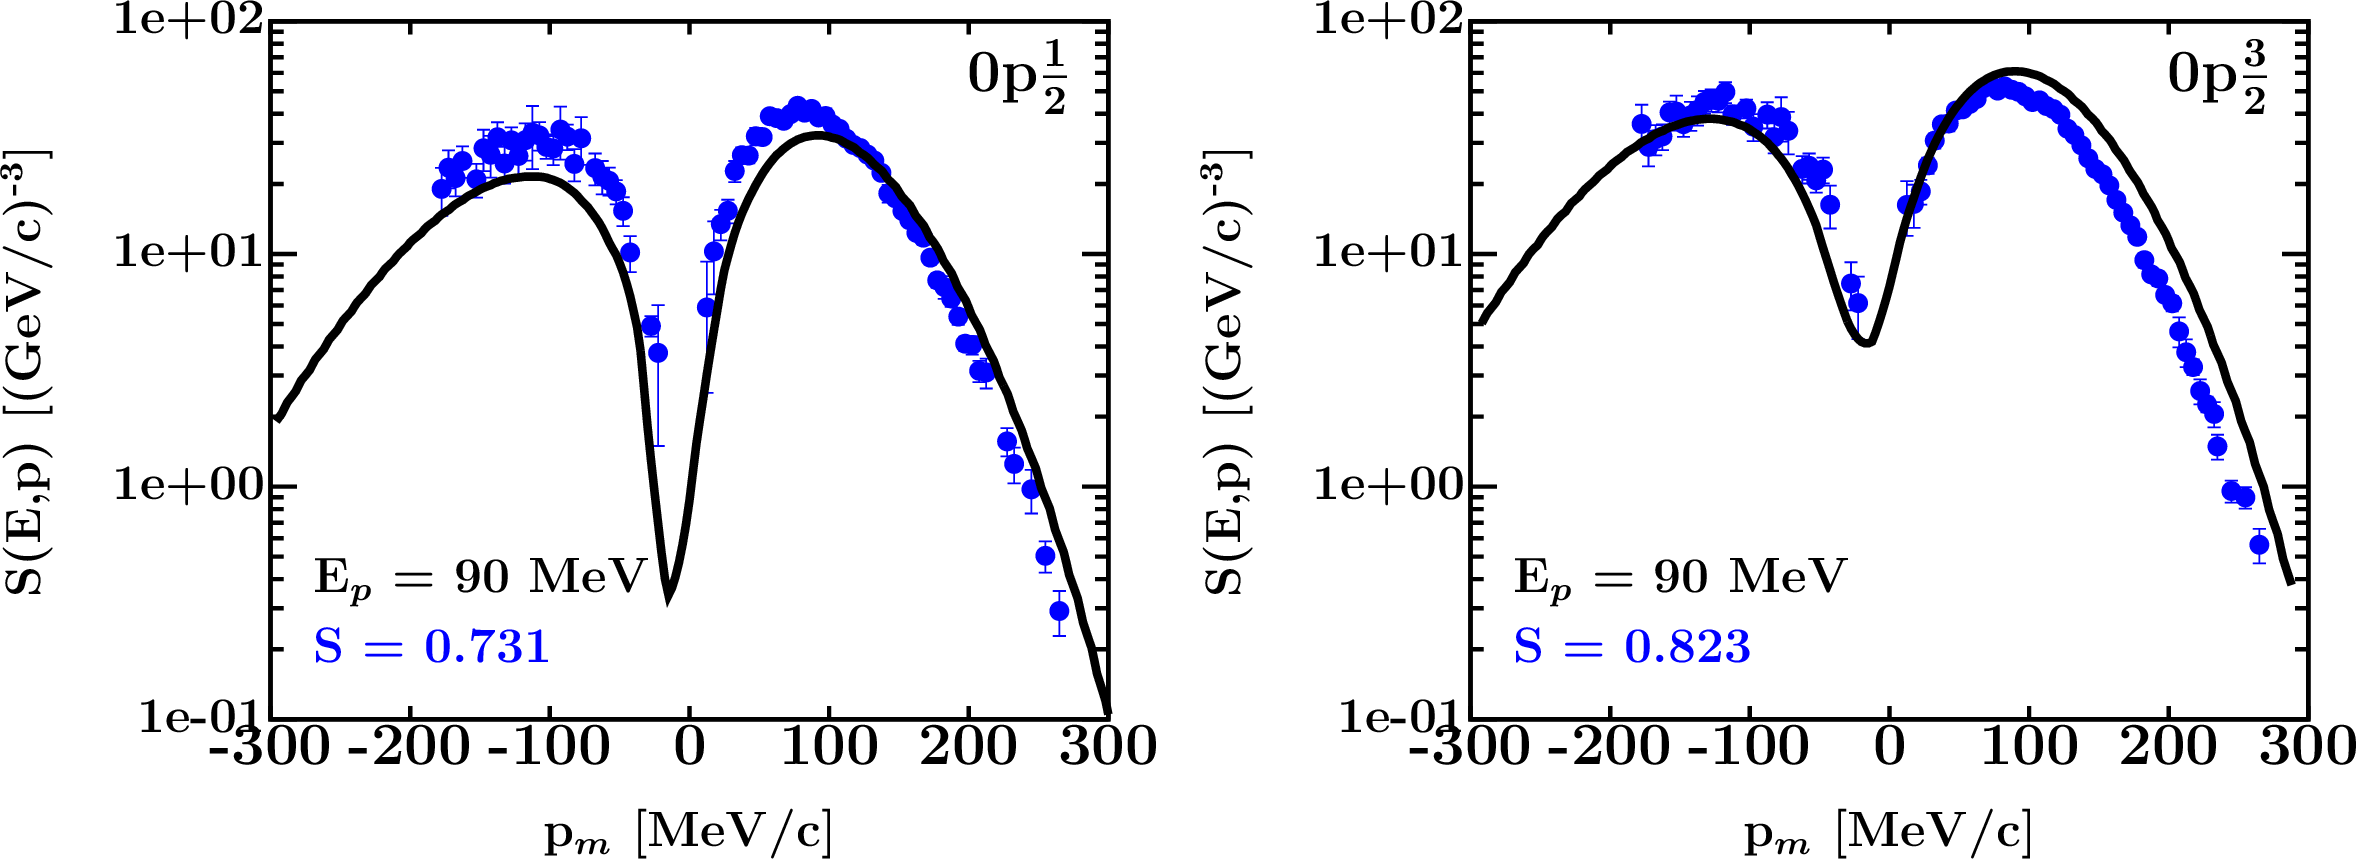
\includegraphics[width = 1.0\textwidth]{figures/o16_eep.png}
    \caption{(e,e'p) cross sections}
    \label{DOMFitData_o16_eep}
\end{figure}

\section{DOM fit of \oEight}
\label{o18DOMOutput}
\begin{figure}[H]
    \centering
    \begin{minipage}{0.45\textwidth}
        \centering
        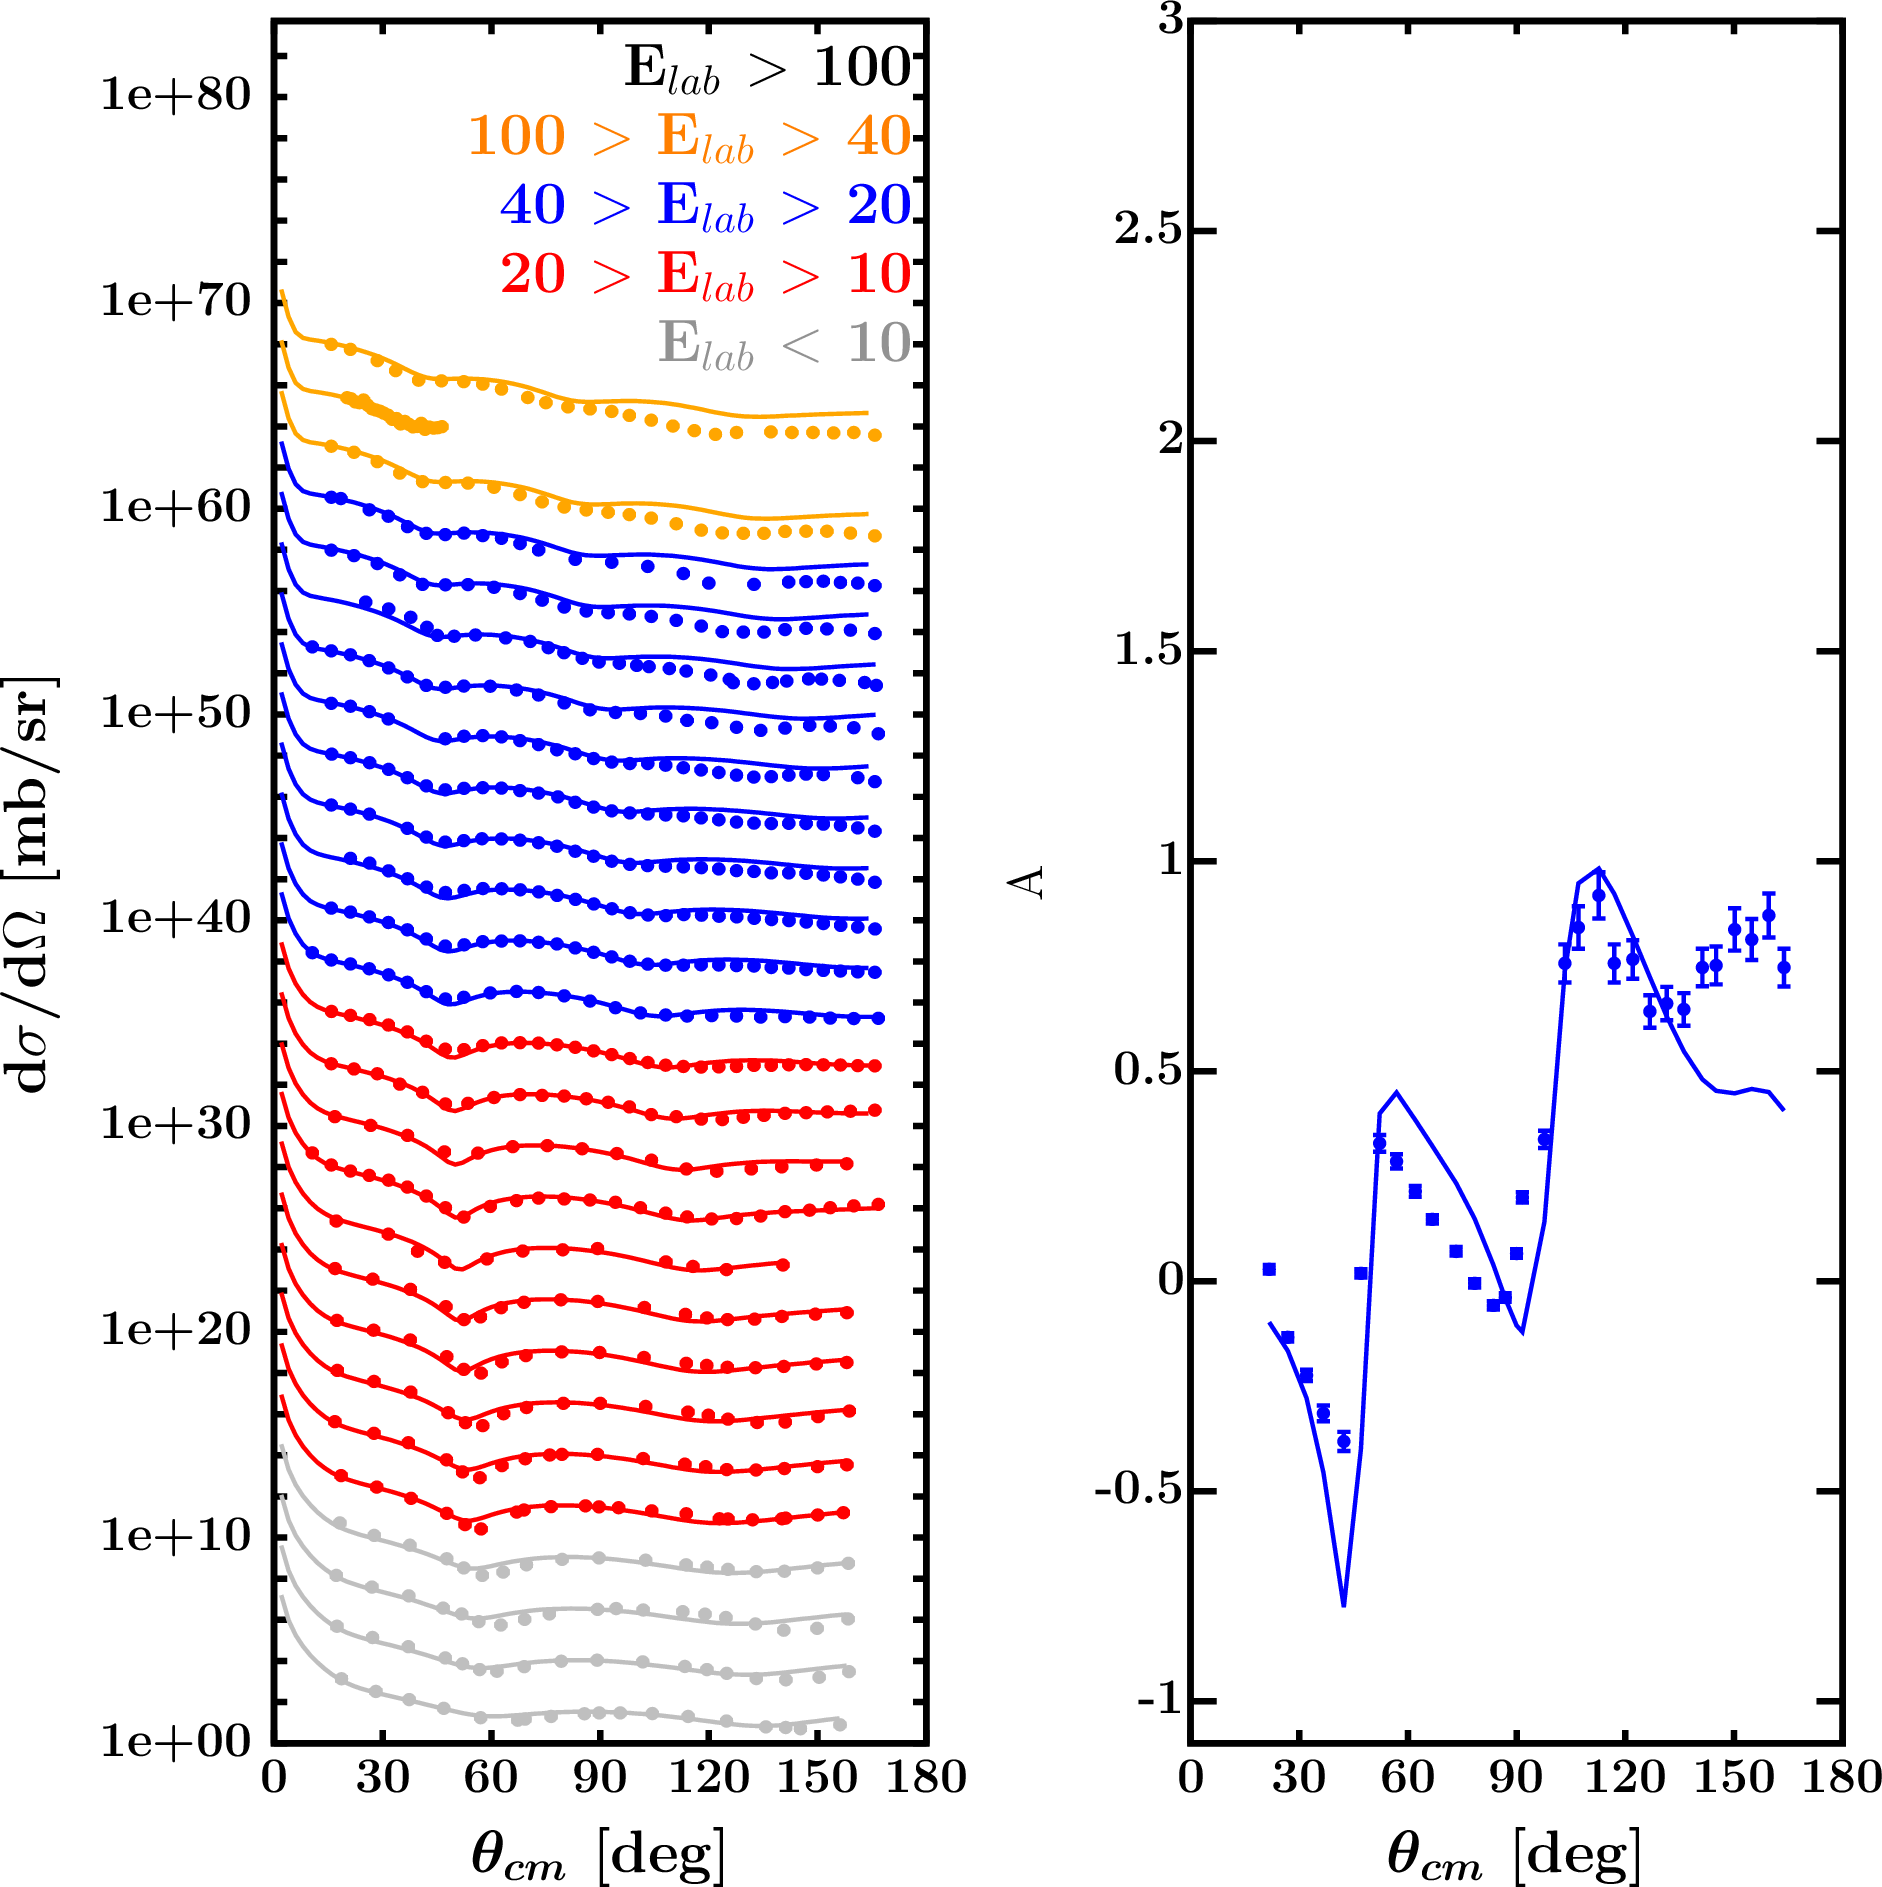
\includegraphics[width=1.0\textwidth]{figures/o18_protonElastic.png}
        \caption{Proton elastic scattering data}
        \label{DOMFitData_o18_proton_elastic}
    \end{minipage}\hfill
    \begin{minipage}{0.45\textwidth}
        \centering
        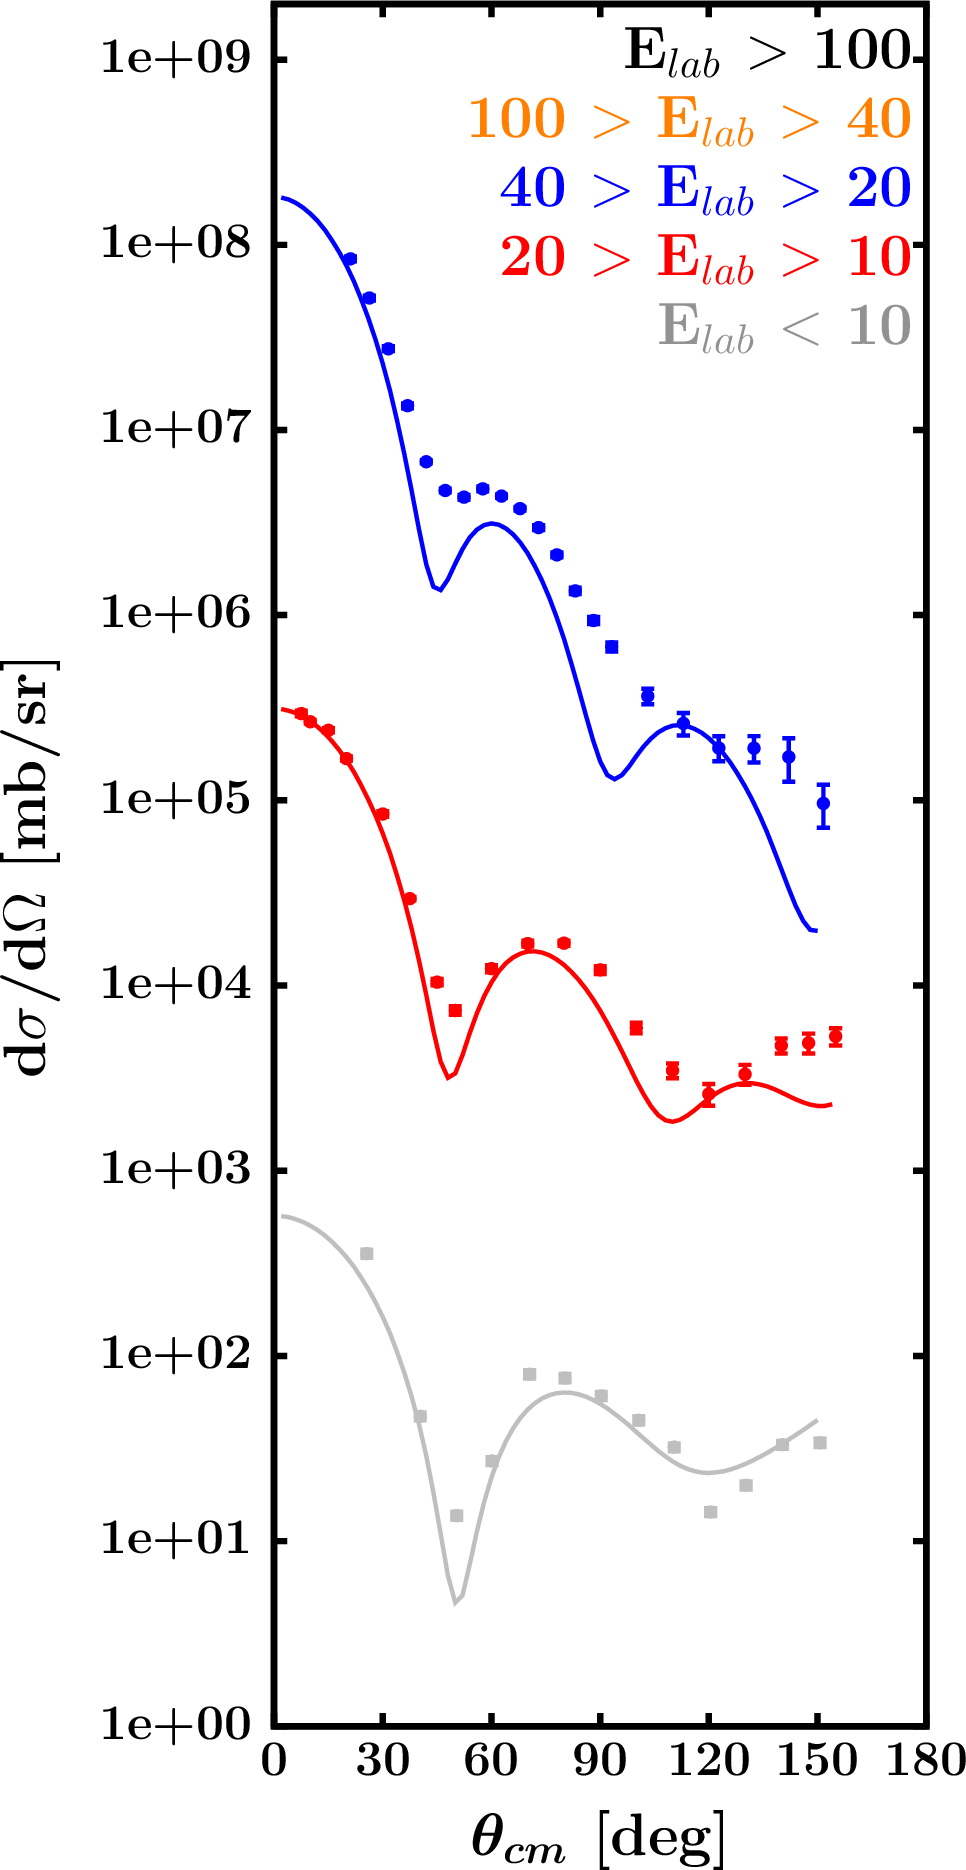
\includegraphics[width=1.0\textwidth]{figures/o18_neutronElastic.png}
        \caption{Neutron elastic scattering data}
        \label{DOMFitData_o18_neutron_elastic}
    \end{minipage}
\end{figure}

\begin{figure}[H]
    \centering
    \begin{minipage}{0.45\textwidth}
        \centering
        
\includegraphics[width=1.0\textwidth]{figures/o18_protonInelastic.png}
        \caption{Proton \rxn data}
        \label{DOMFitData_o18_proton_inelastic}
    \end{minipage}\hfill
    \begin{minipage}{0.45\textwidth}
        \centering
        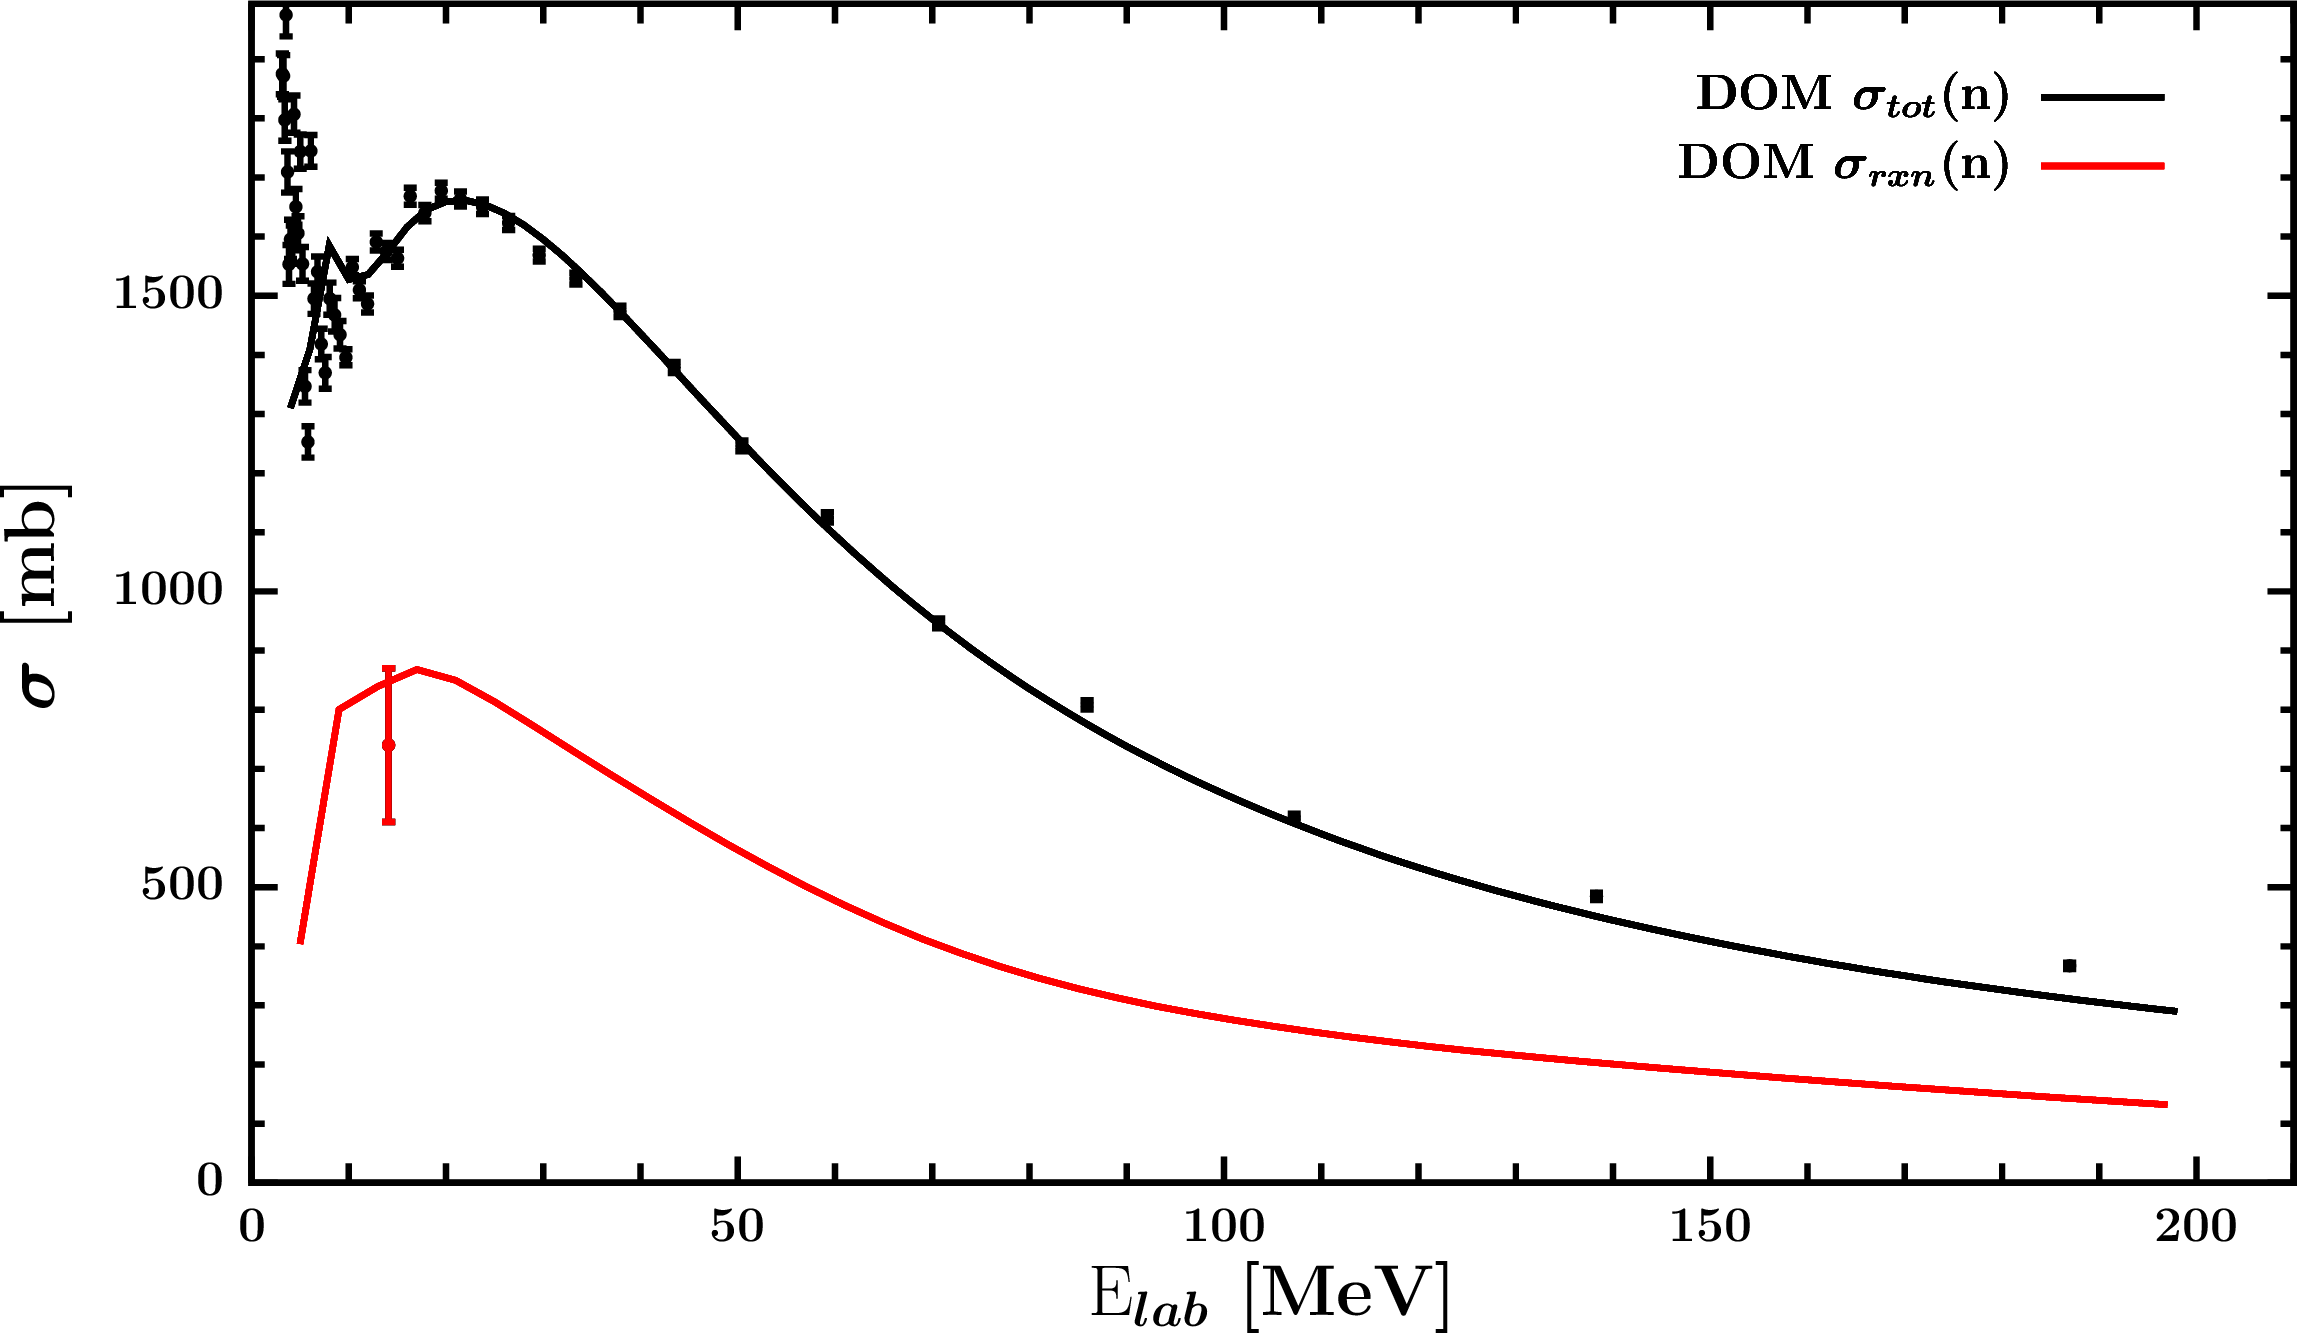
\includegraphics[width=1.0\textwidth]{figures/o18_neutronInelastic.png}
        \caption{Neutron \rxn and \tot data}
        \label{DOMFitData_o18_neutron_inelastic}
    \end{minipage}
\end{figure}

\afterpage{\clearpage}

\begin{figure}[H]
    \centering
    \begin{minipage}{0.45\textwidth}
        \centering
        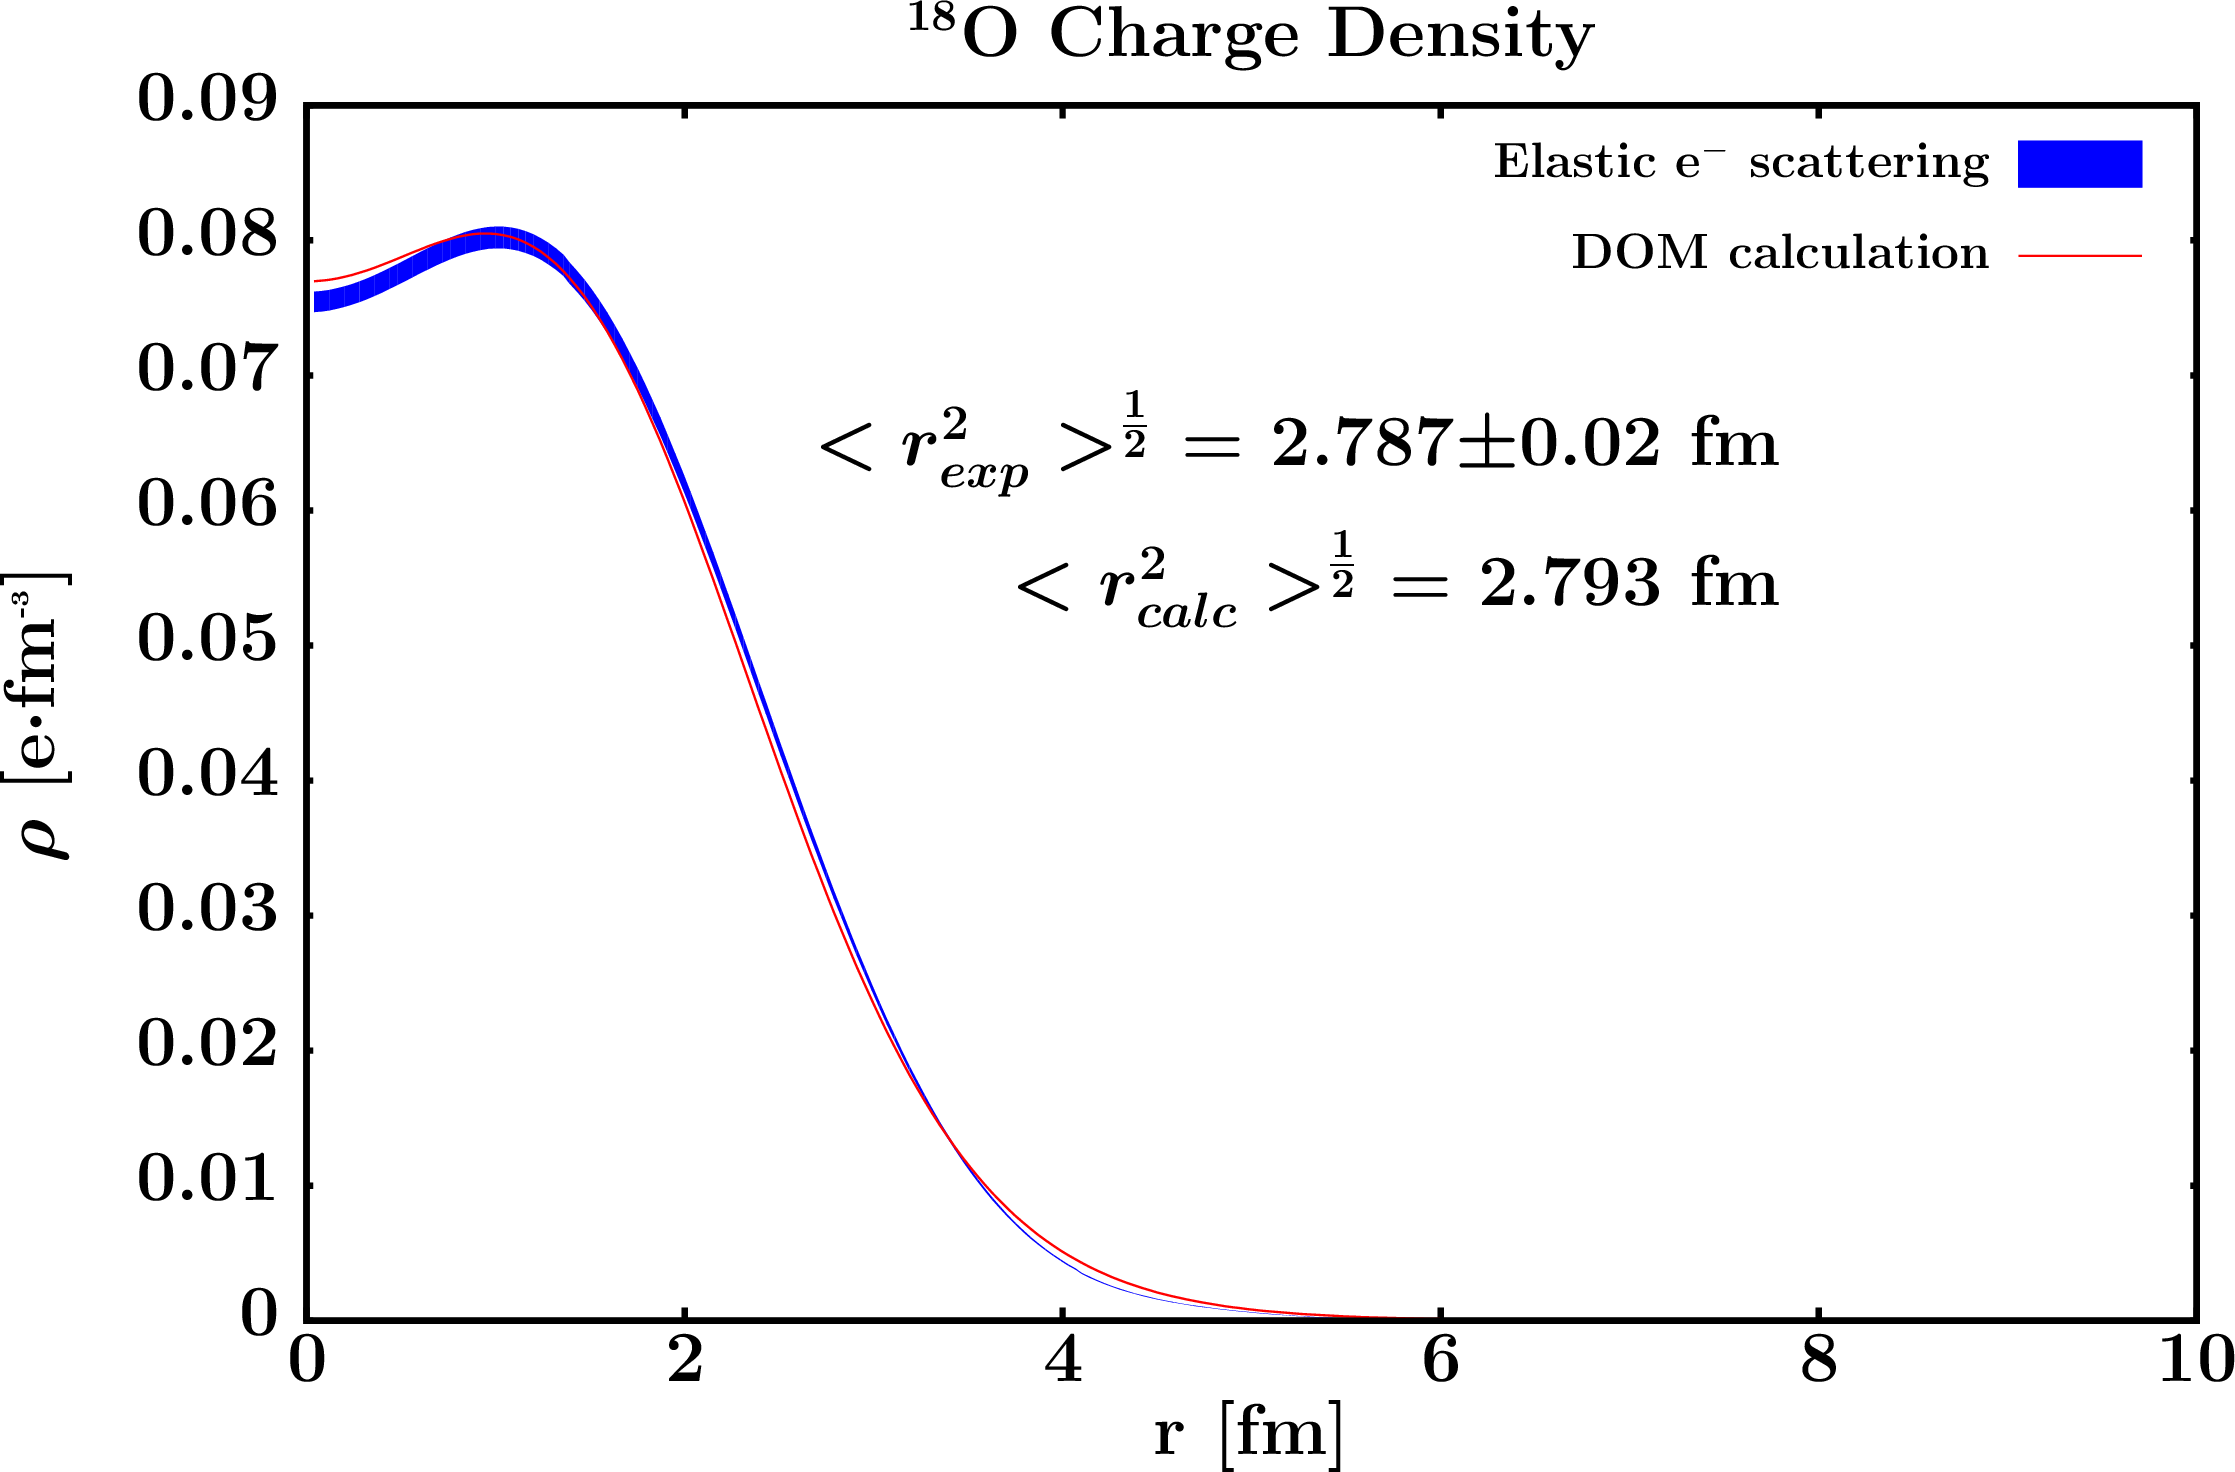
\includegraphics[width=1.0\textwidth]{figures/o18_chargeDensity.png}
        \caption{Charge density data}
        \label{DOMFitData_o18_chargeDensity}
    \end{minipage}\hfill
    \begin{minipage}{0.45\textwidth}
        \centering
        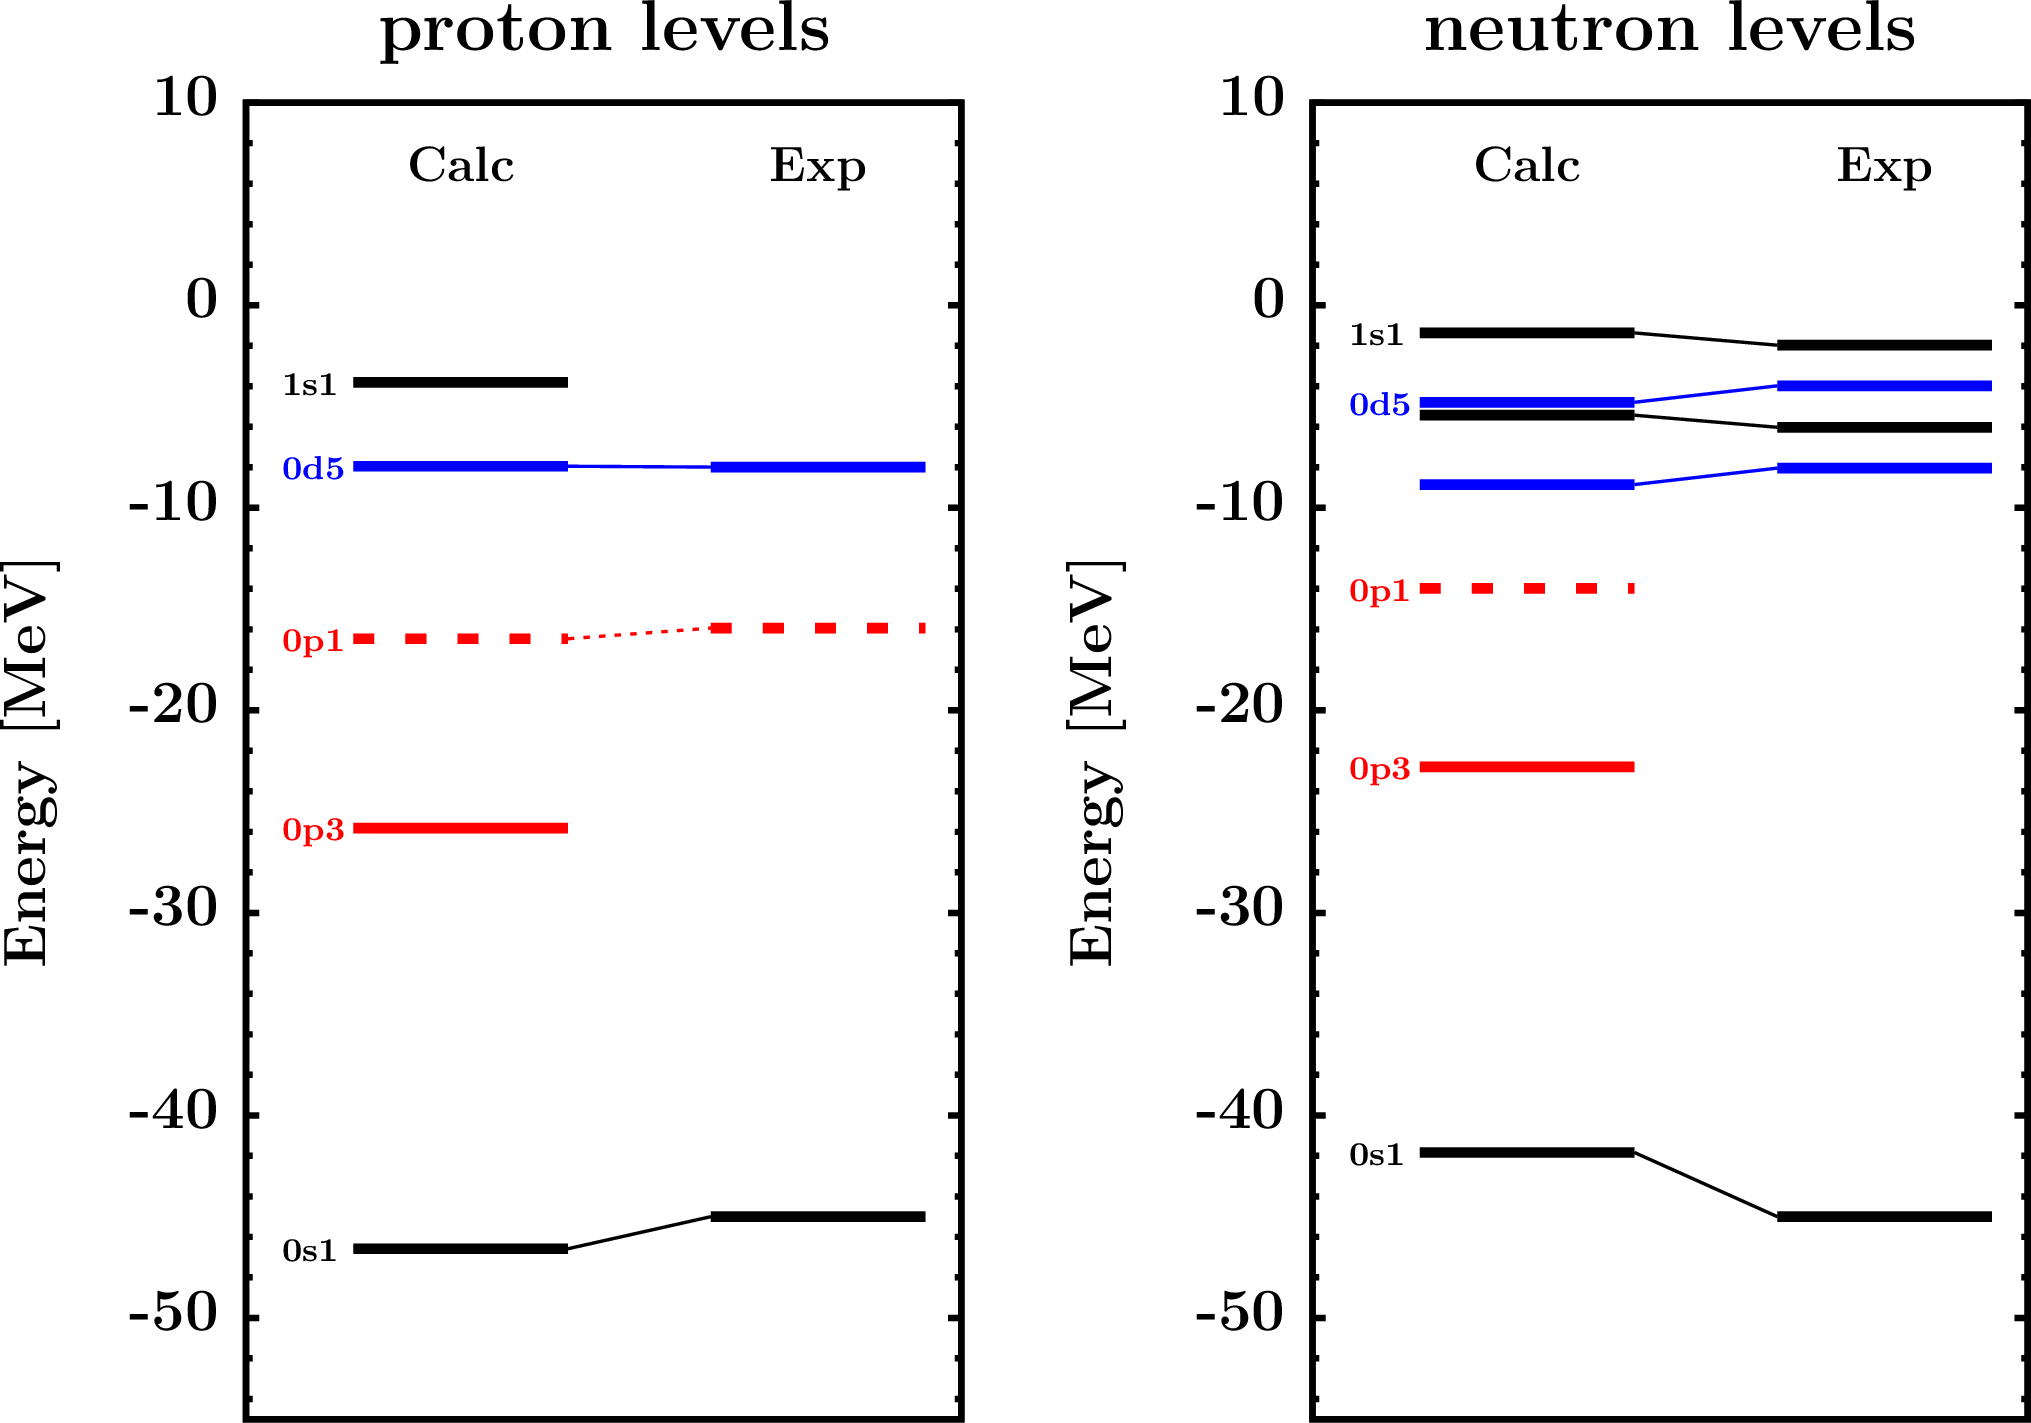
\includegraphics[width=1.0\textwidth]{figures/o18_SPLevels.png}
        \caption{Single-particle levels}
        \label{DOMFitData_o18_SPLevels}
    \end{minipage}
\end{figure}

\afterpage{\clearpage}

\begin{figure}[H]
    \centering
    \begin{minipage}{0.45\textwidth}
        \centering
        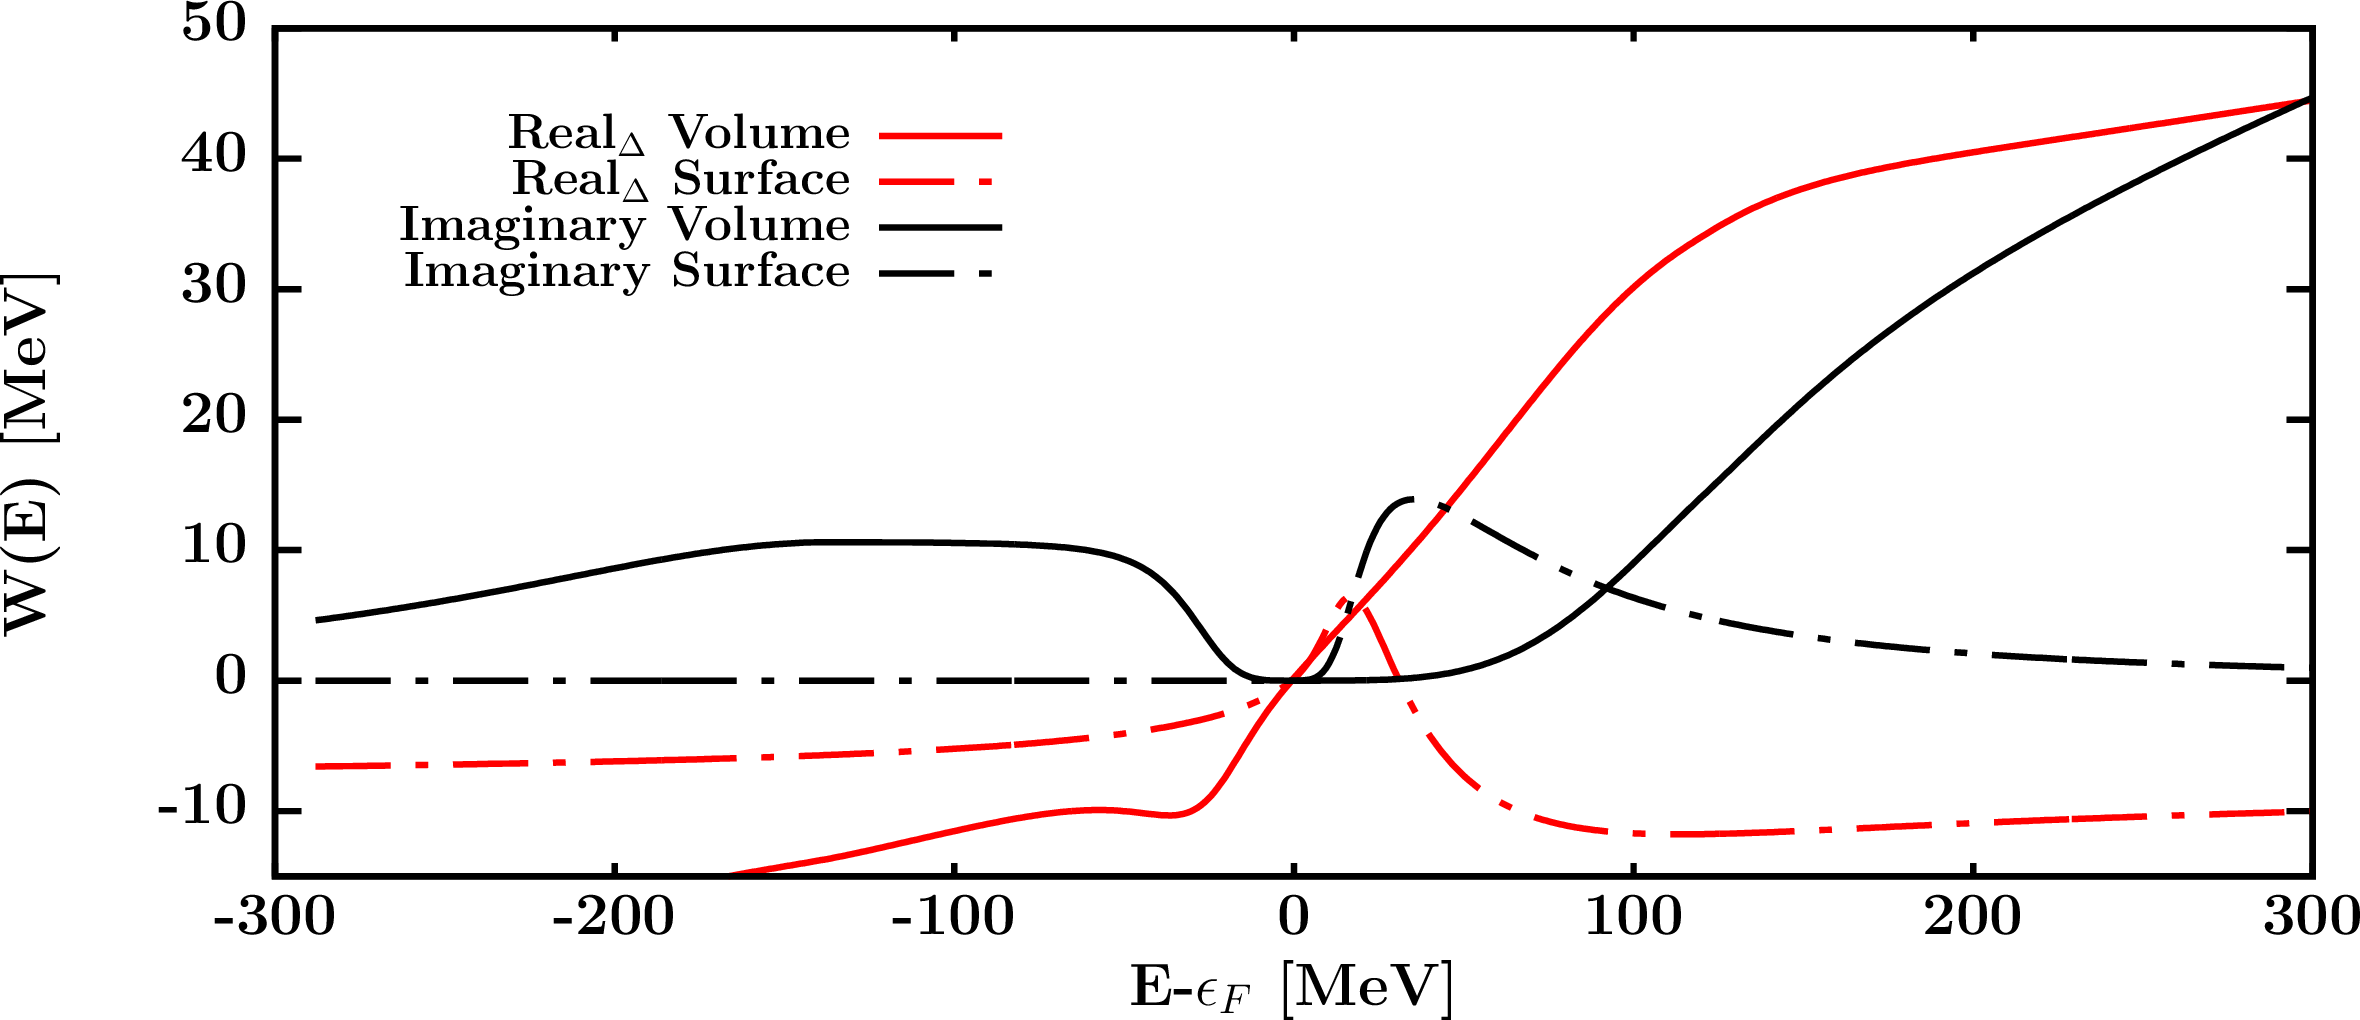
\includegraphics[width=1.0\textwidth]{figures/o18_protonPotentials.png}
        \caption{Energy-dependence of optical potential components for protons
        on \oEight}
        \label{DOMFitData_o18_proton_potentialComponent_energy}
    \end{minipage}\hfill
    \begin{minipage}{0.45\textwidth}
        \centering
        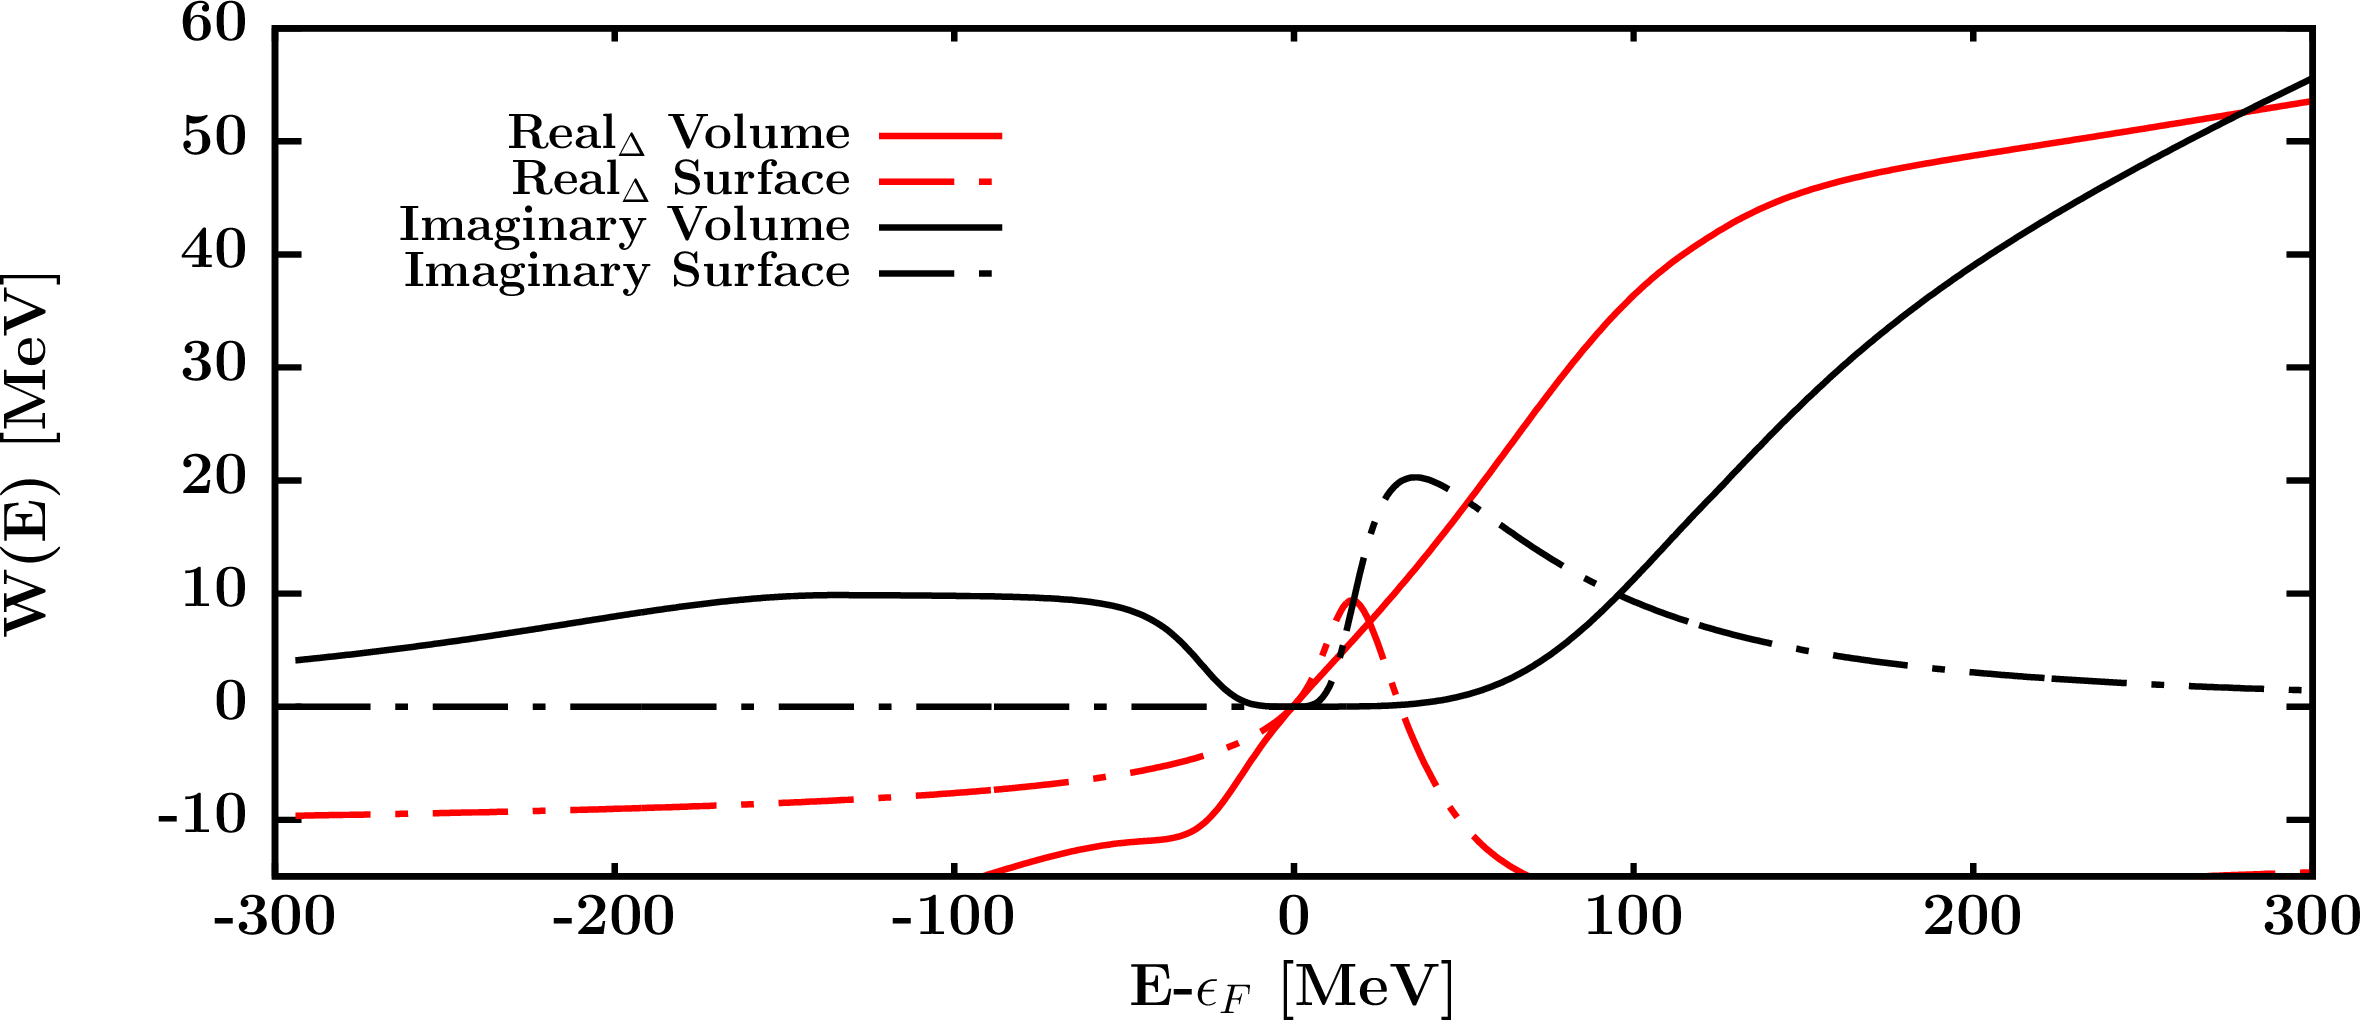
\includegraphics[width=1.0\textwidth]{figures/o18_neutronPotentials.png}
        \caption{Neutron potential energy-dependent component}
        \label{DOMFitData_o18_neutron_potentialComponent_energy}
    \end{minipage}
\end{figure}

\begin{figure}[H]
    \centering
    \begin{minipage}{0.45\textwidth}
        \centering
        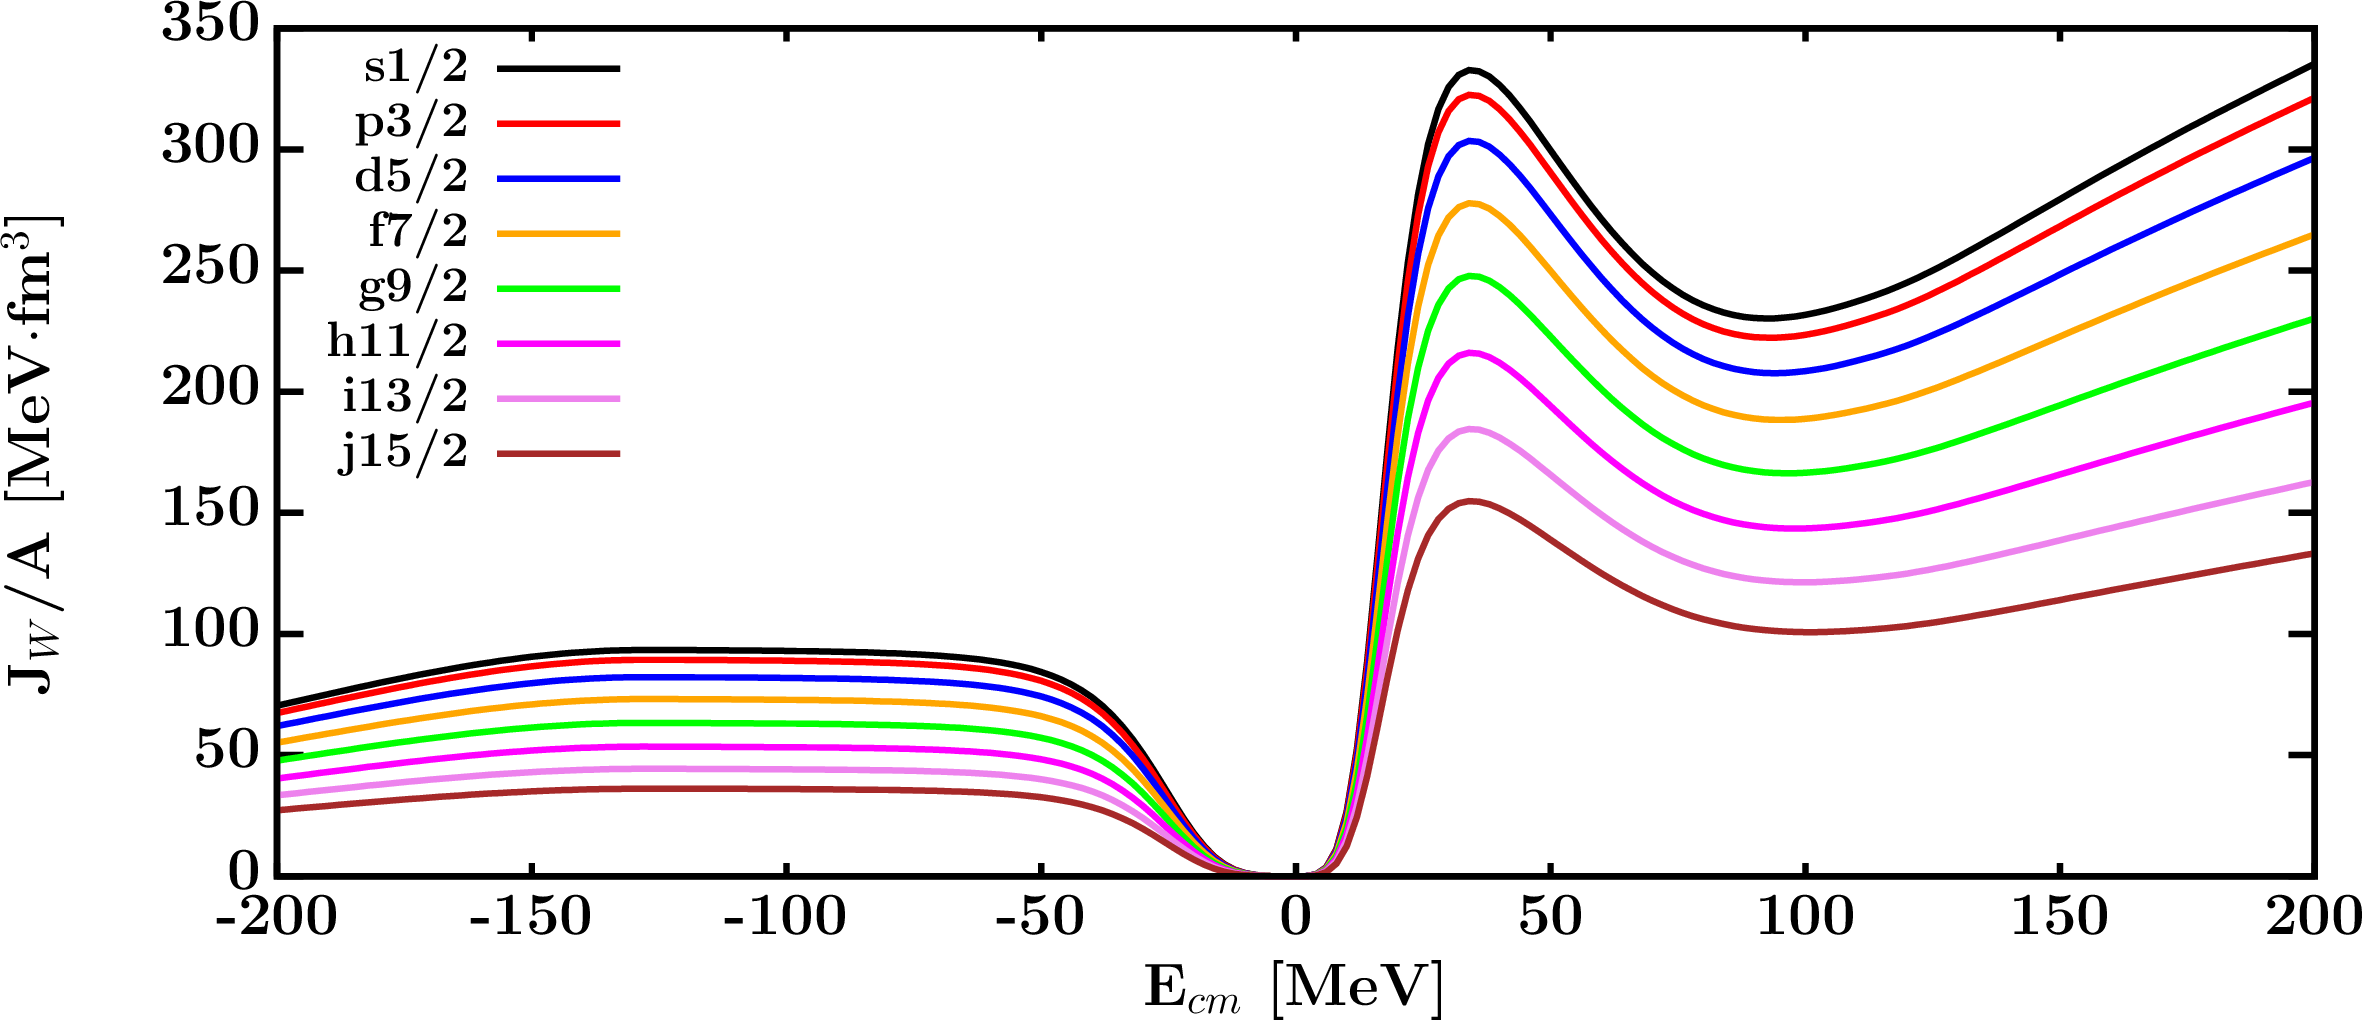
\includegraphics[width=1.0\textwidth]{figures/o18_protonVolumeIntegrals.png}
        \caption{Proton potential, integrated over r-space}
        \label{DOMFitData_o18_proton_potentialIntegral}
    \end{minipage}\hfill
    \begin{minipage}{0.45\textwidth}
        \centering
        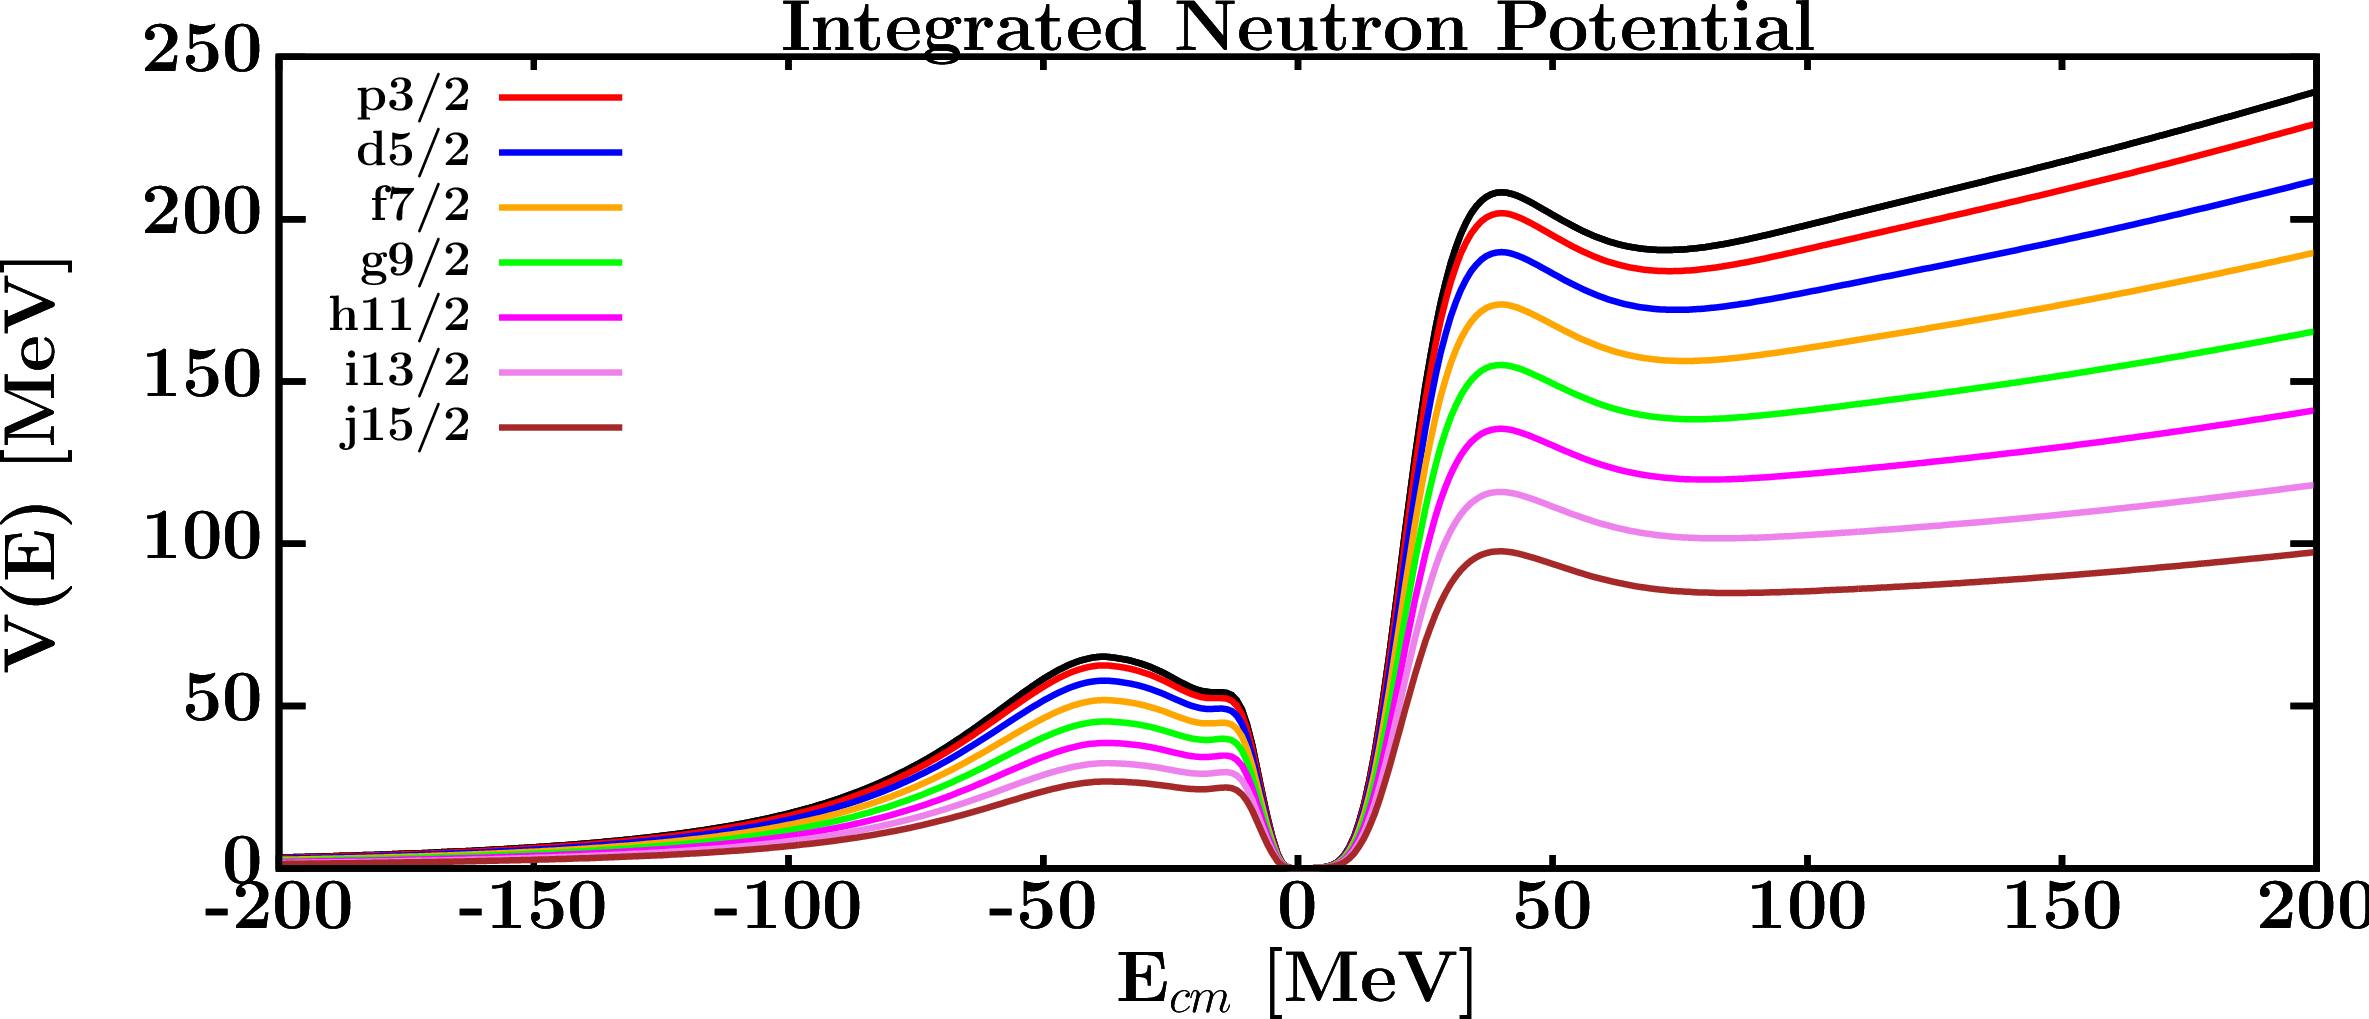
\includegraphics[width=1.0\textwidth]{figures/o18_neutronVolumeIntegrals.png}
        \caption{Neutron potential, integrated over r-space}
        \label{DOMFitData_o18_neutron_potentialIntegral}
    \end{minipage}
\end{figure}

\afterpage{\clearpage}

\begin{figure}[H]
    \centering
    \begin{minipage}{0.45\textwidth}
        \centering
        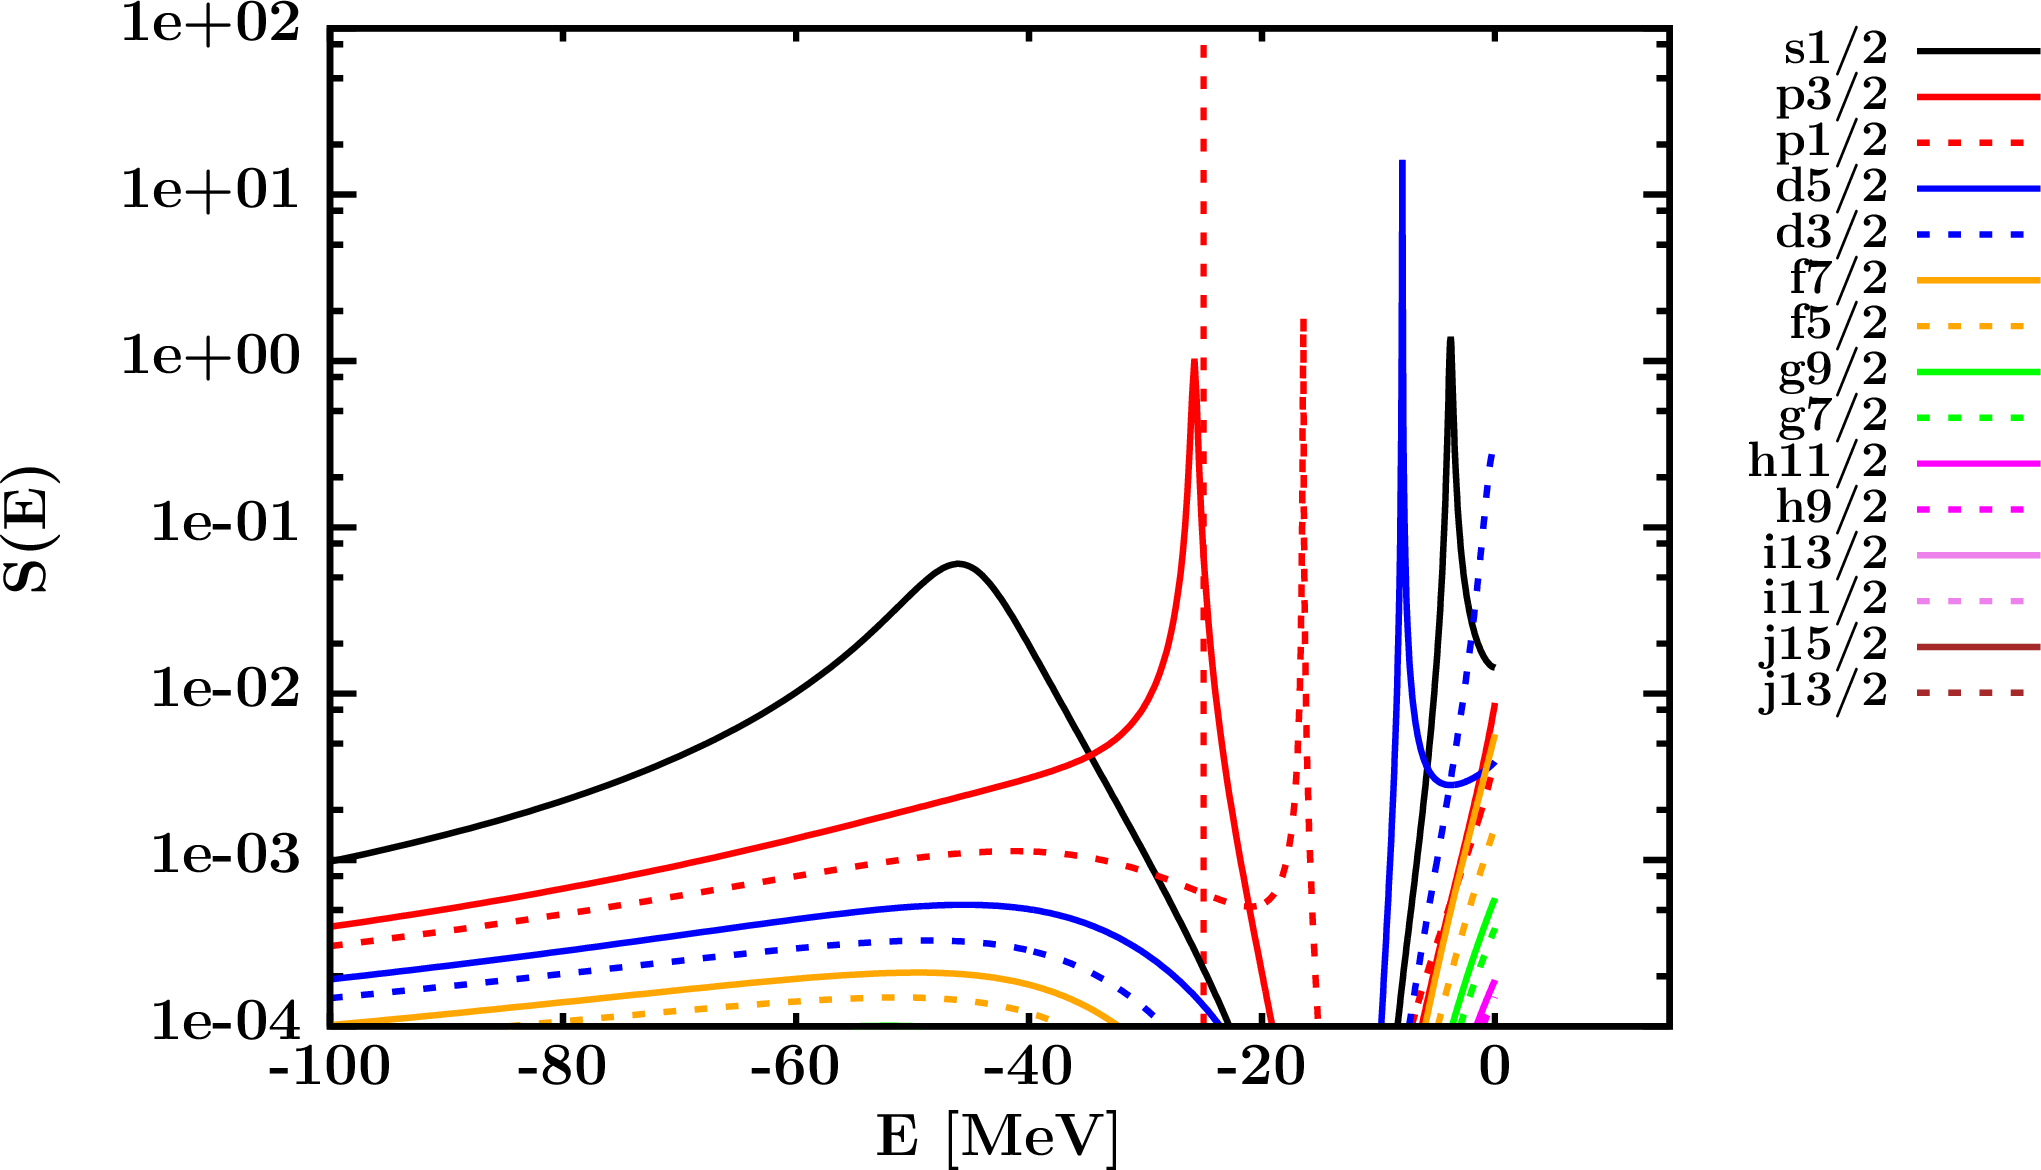
\includegraphics[width=1.0\textwidth]{figures/o18_protonSpectralFunctions.png}
        \caption{Proton spectral functions}
        \label{DOMFitData_o18_proton_spectralFunctions}
    \end{minipage}\hfill
    \begin{minipage}{0.45\textwidth}
        \centering
        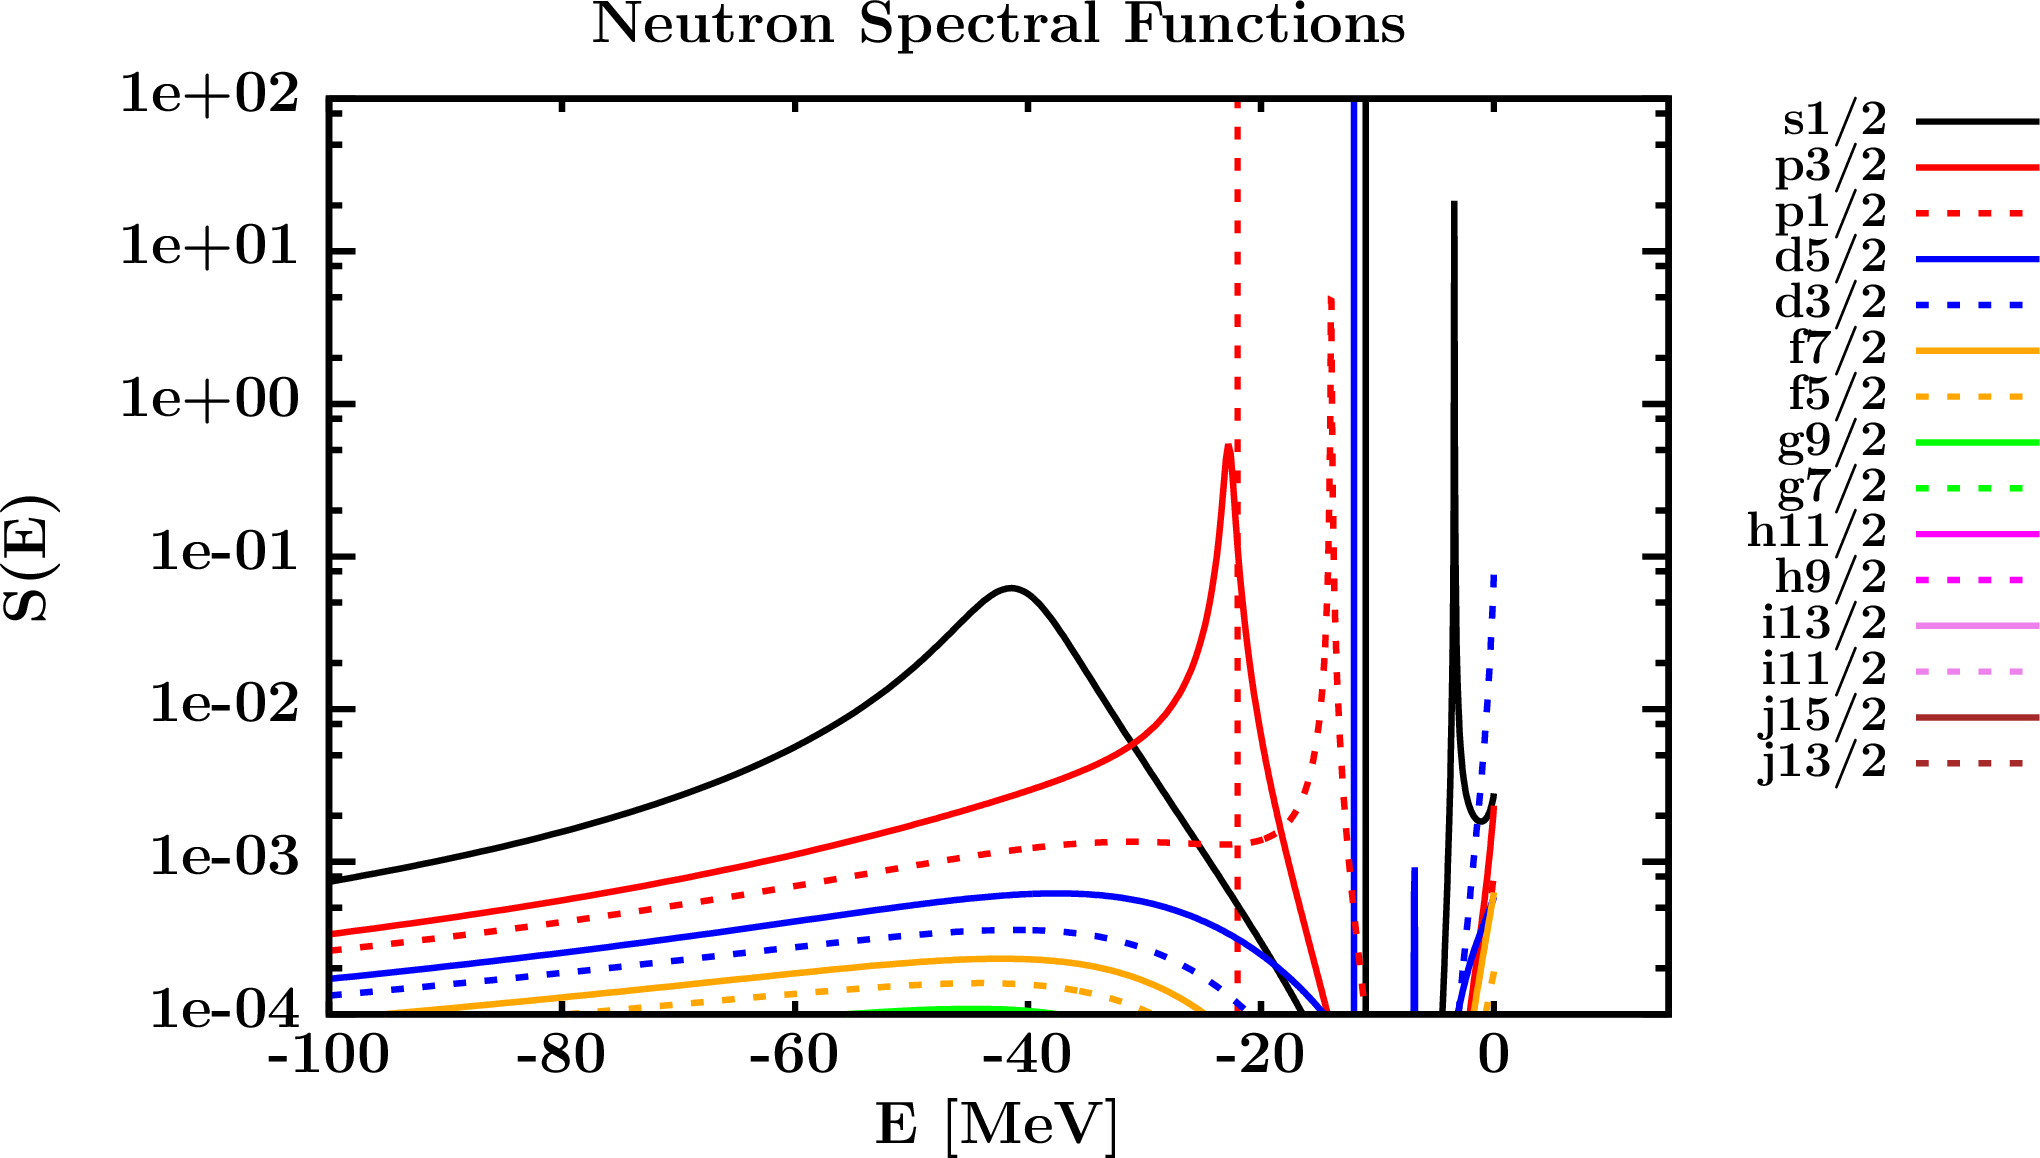
\includegraphics[width=1.0\textwidth]{figures/o18_neutronSpectralFunctions.png}
        \caption{Neutron spectral functions}
        \label{DOMFitData_o18_neutron_spectralFunctions}
    \end{minipage}
\end{figure}

\begin{figure}[H]
    \centering
    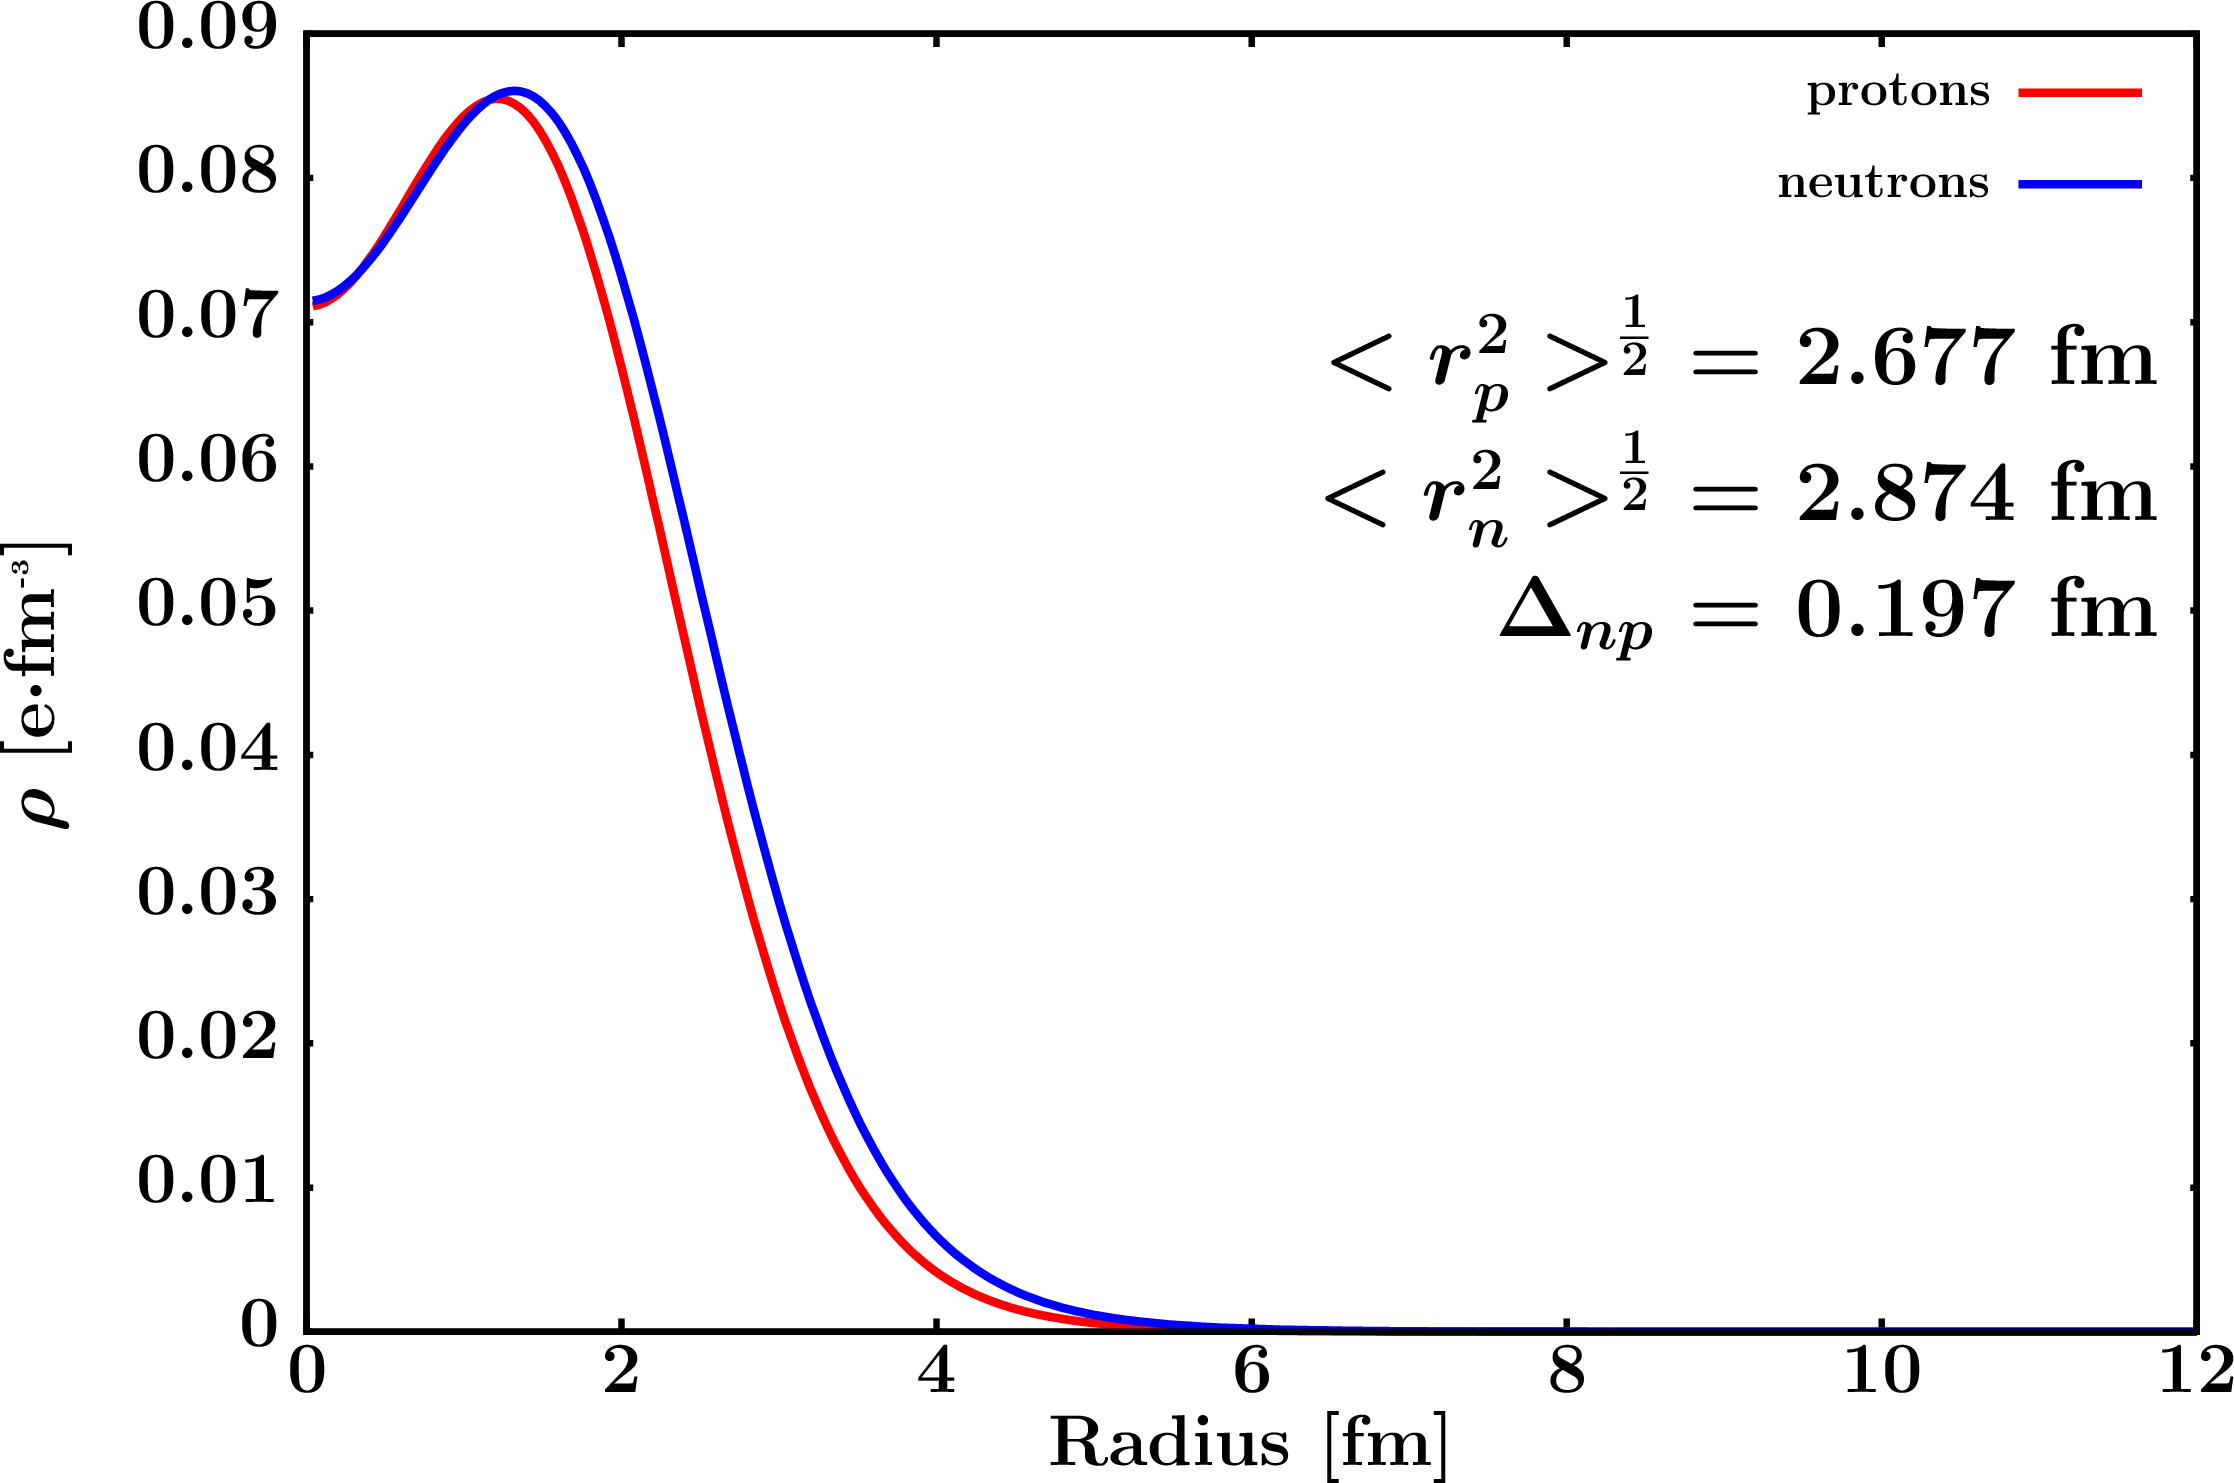
\includegraphics[width = 0.5\textwidth]{figures/o18_matterDensity.png}
    \caption{Matter density distribution}
    \label{DOMFitData_o18_matterDensity}
\end{figure}

\begin{figure}[H]
    \centering
    \includegraphics[width = 0.5\textwidth]{figures/o18_momentumDistribution.png}
    \caption{Momentum distribution}
    \label{DOMFitData_o18_momentumDistribution}
\end{figure}

\begin{figure}[H]
    \centering
    \includegraphics[width = 0.5\textwidth]{figures/o18_energyDensity.png}
    \caption{Energy density distribution}
    \label{DOMFitData_o18_energyDensity}
\end{figure}

\section{DOM fit of \caForty}

\label{ca40DOMOutput}
\begin{figure}[H]
    \centering
    \begin{minipage}{0.45\textwidth}
        \centering
        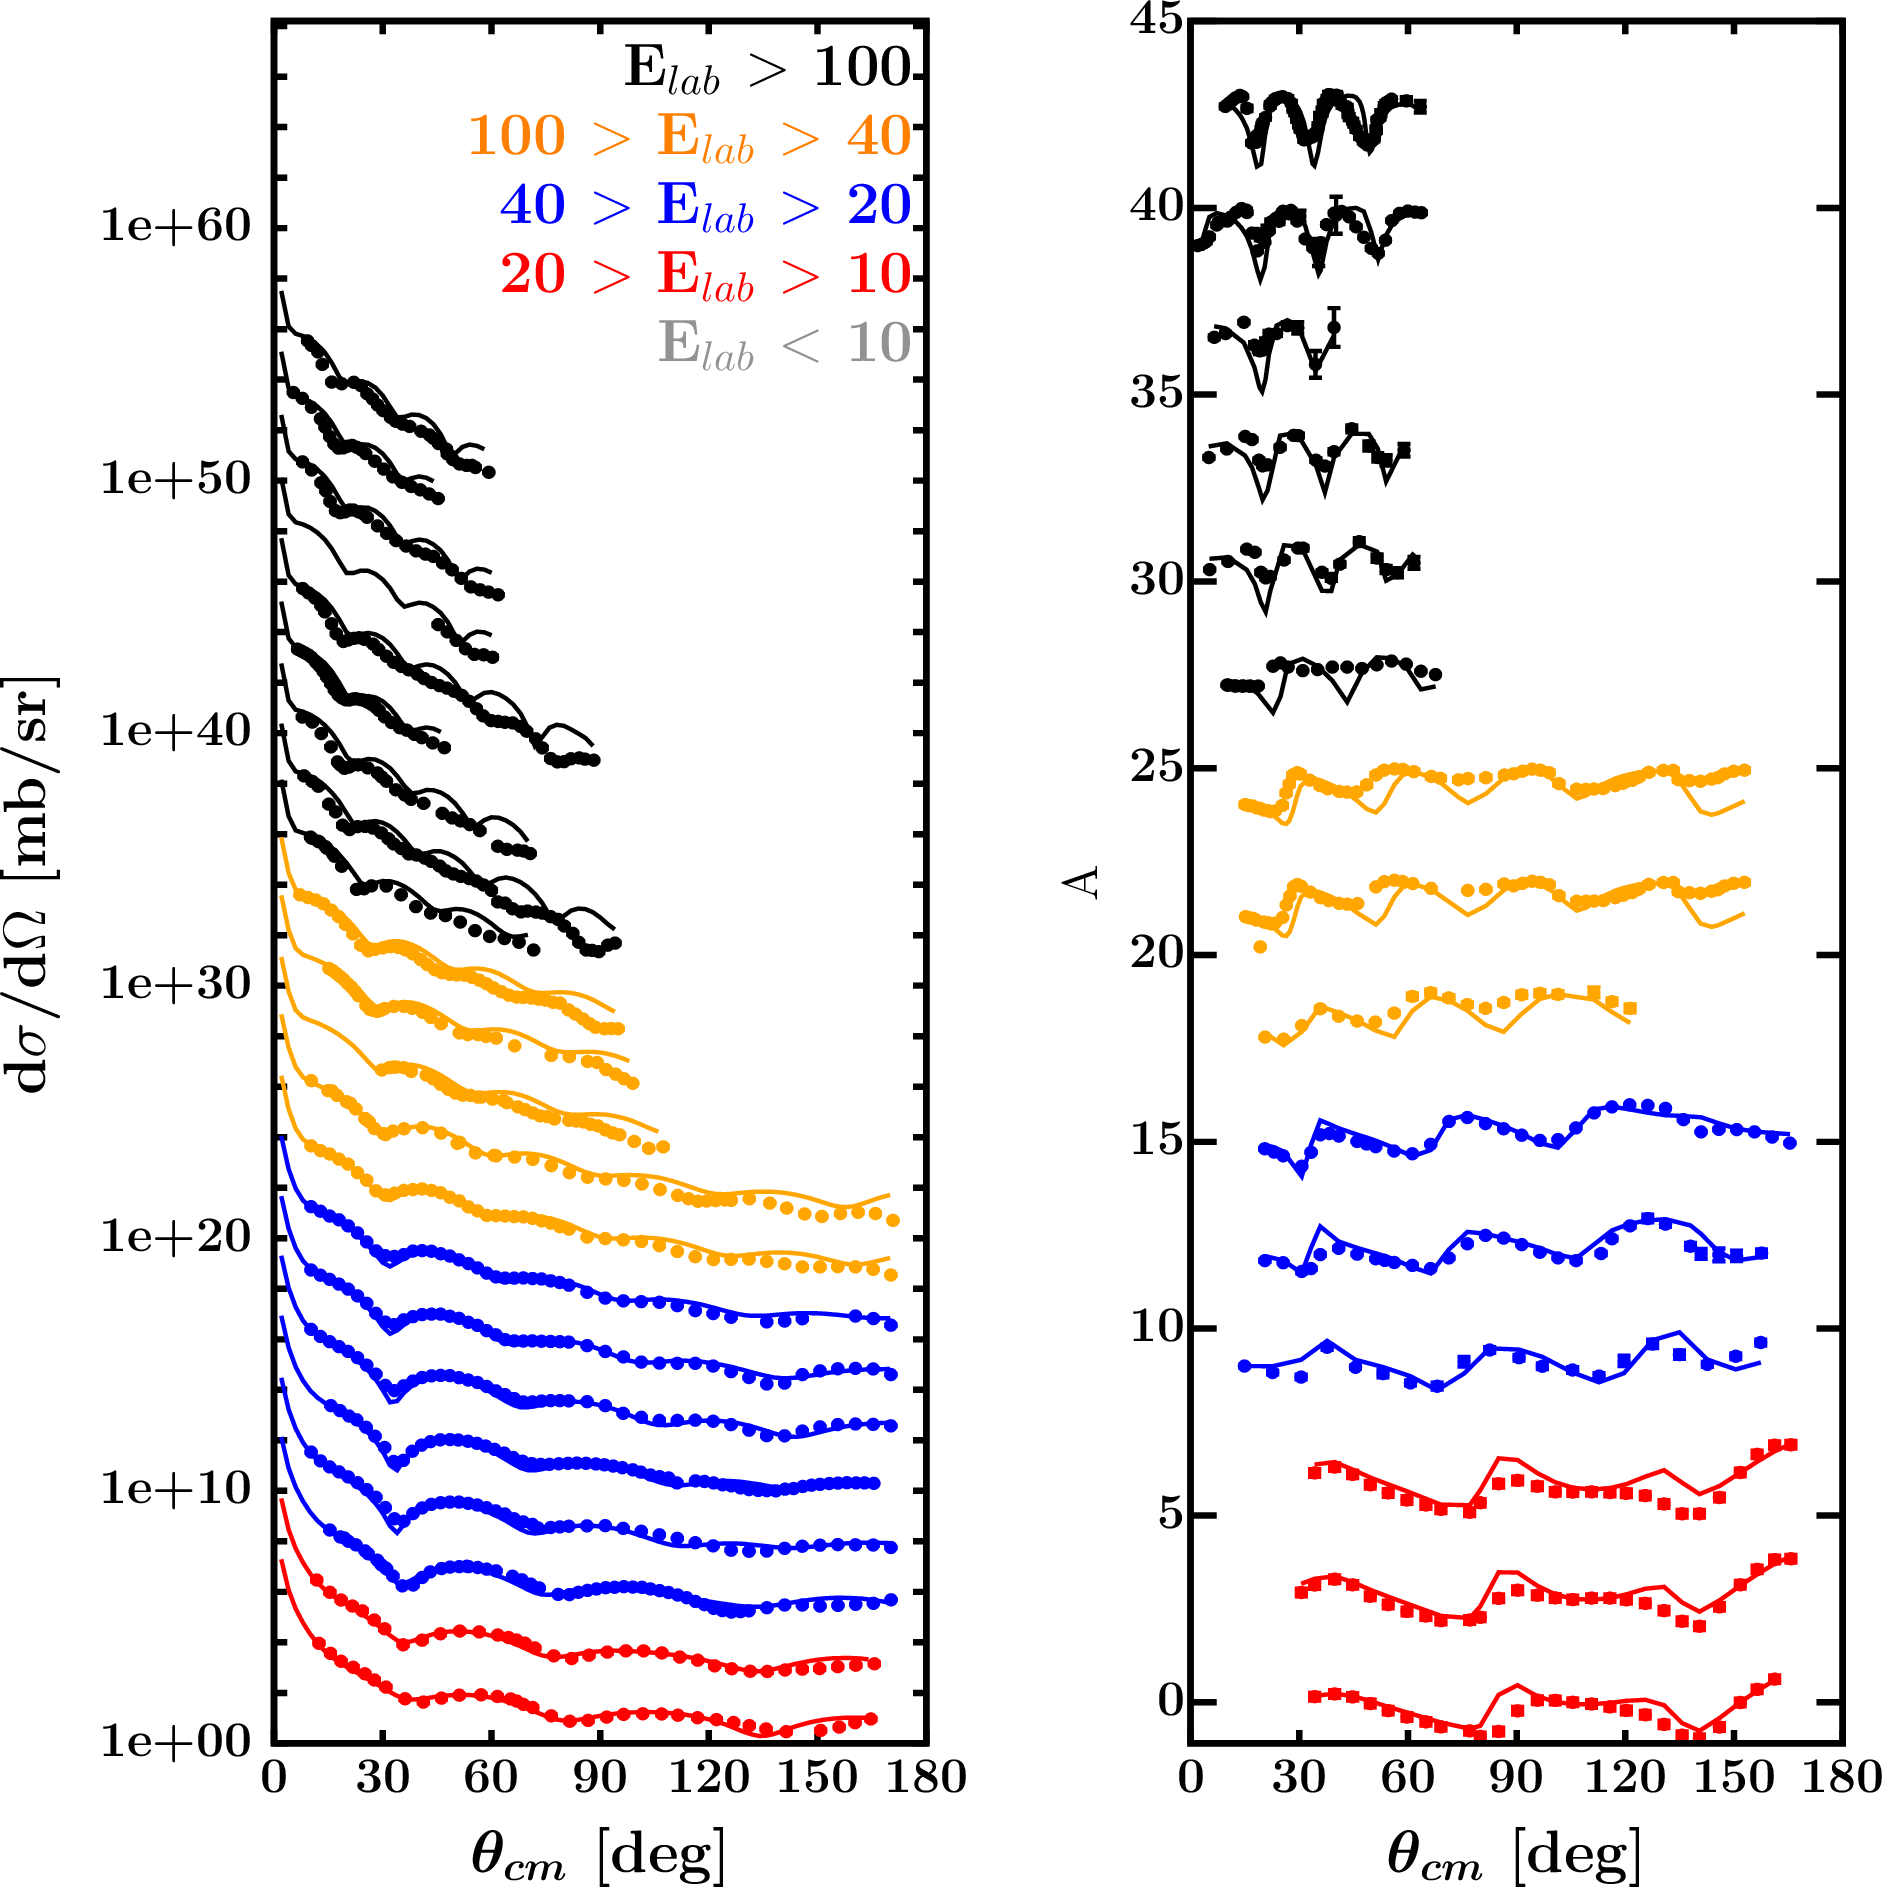
\includegraphics[width=1.0\textwidth]{figures/ca40_protonElastic.png}
        \caption{Proton elastic scattering data}
        \label{DOMFitData_ca40_proton_elastic}
    \end{minipage}\hfill
    \begin{minipage}{0.45\textwidth}
        \centering
        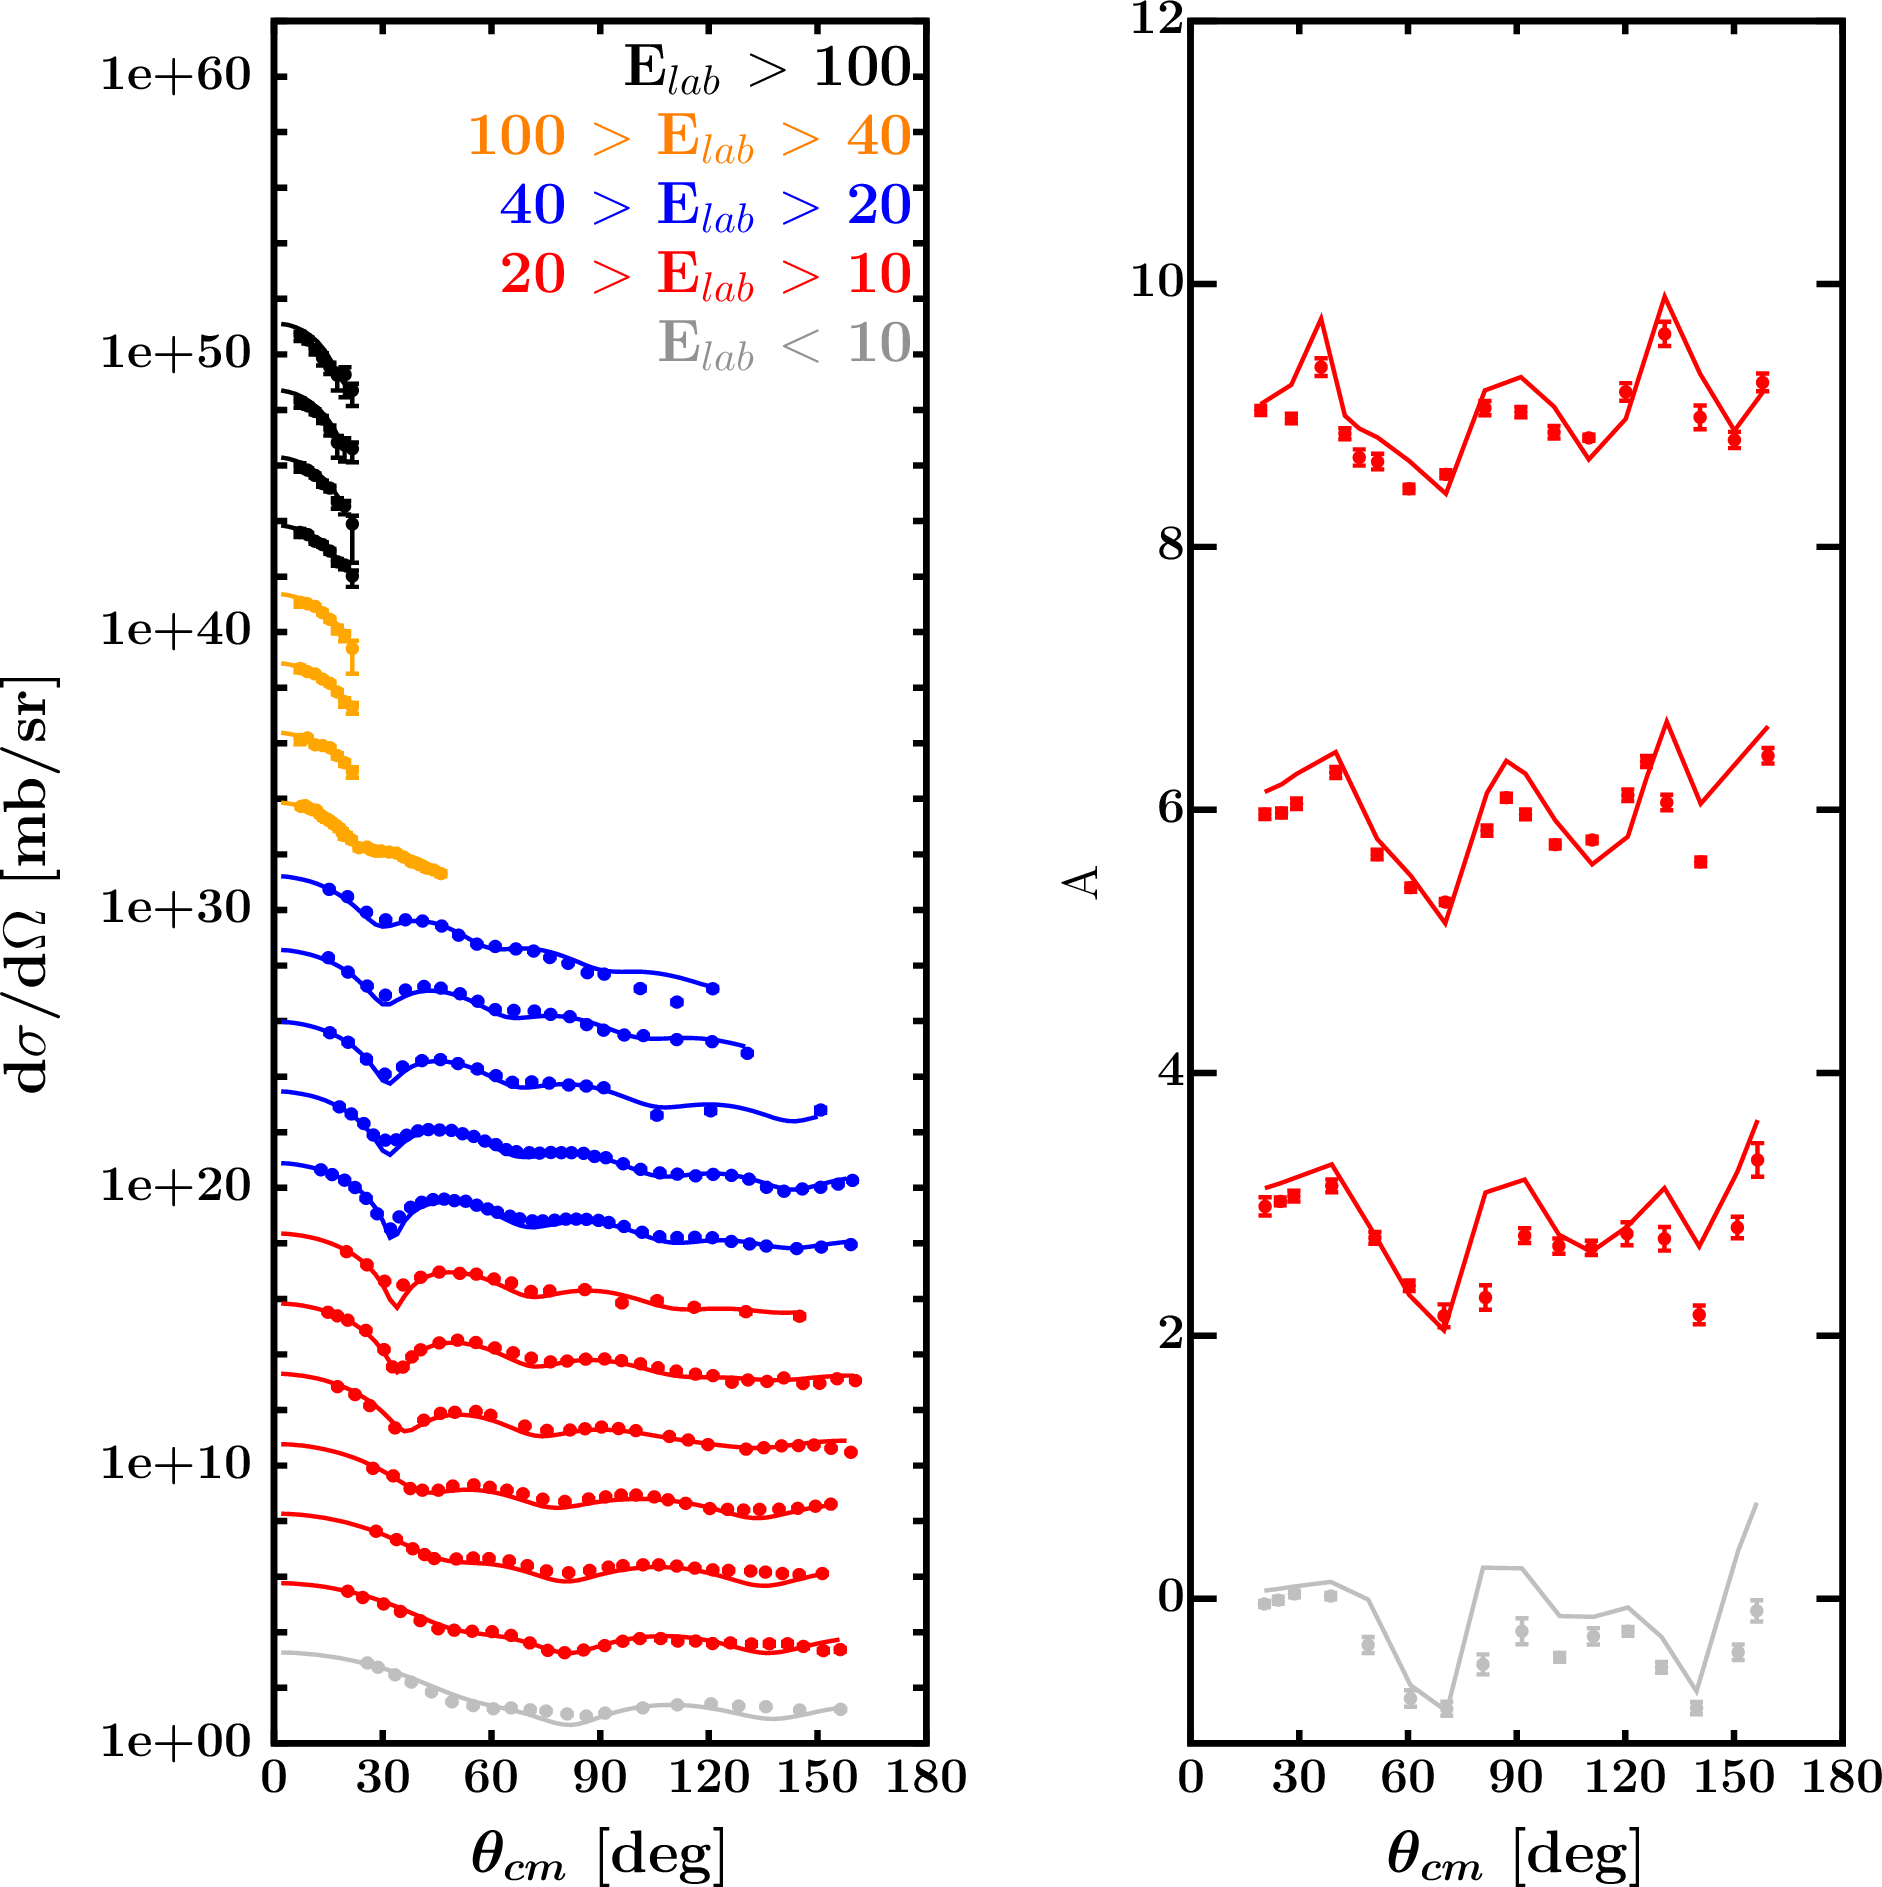
\includegraphics[width=1.0\textwidth]{figures/ca40_neutronElastic.png}
        \caption{Neutron elastic scattering data}
        \label{DOMFitData_ca40_neutron_elastic}
    \end{minipage}
\end{figure}

\begin{figure}[H]
    \centering
    \begin{minipage}{0.45\textwidth}
        \centering
        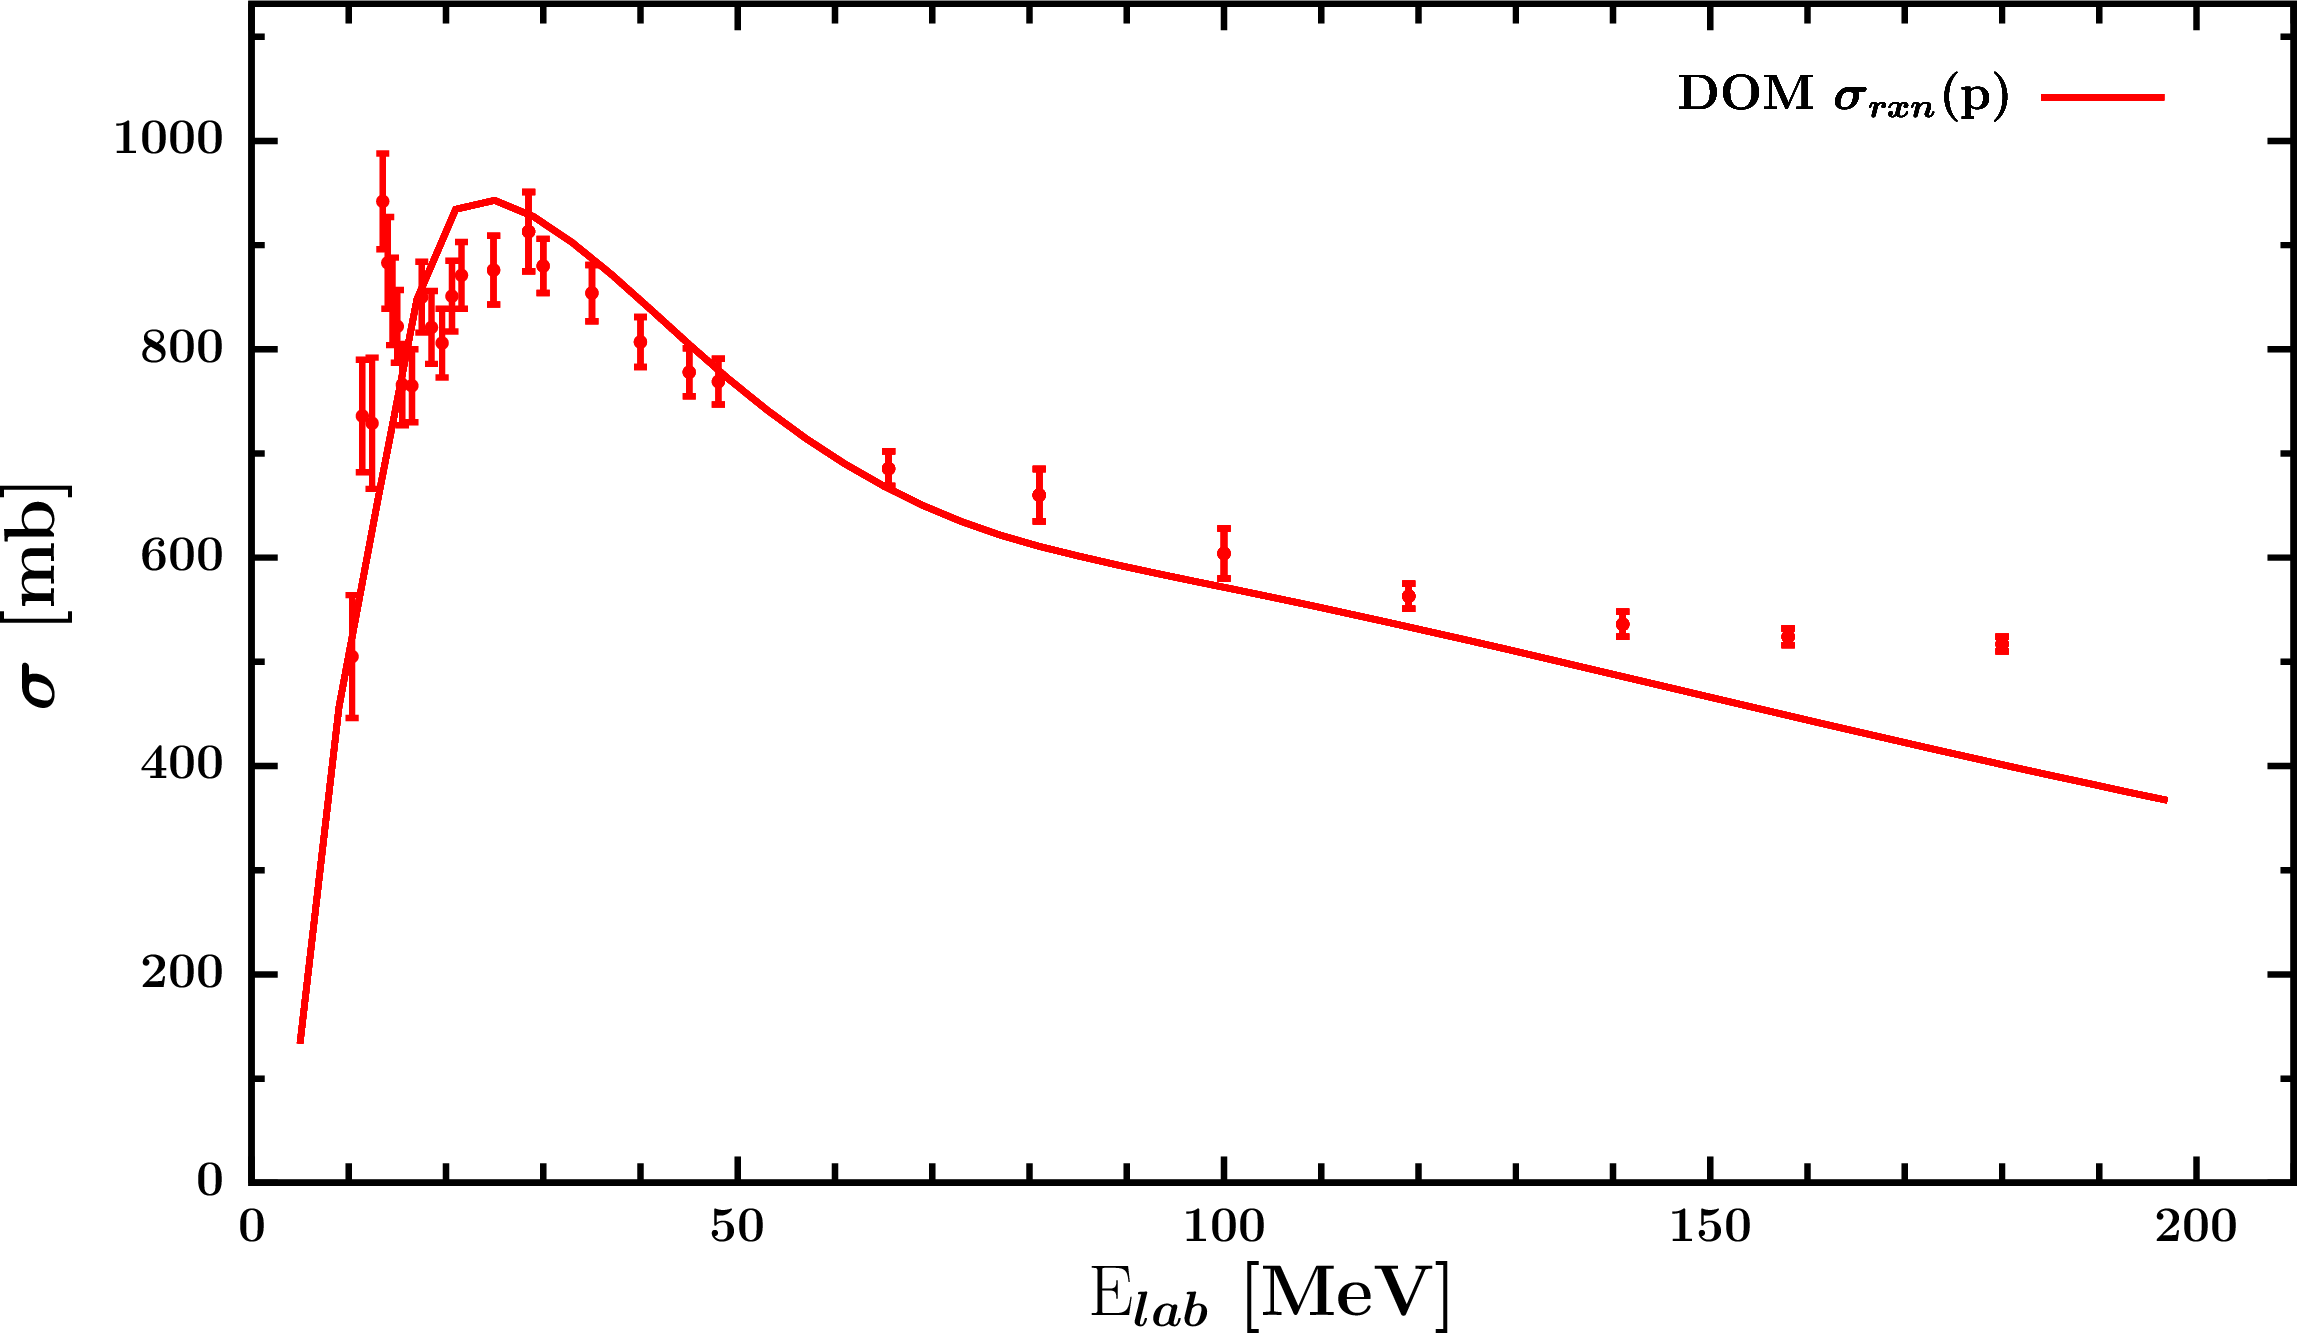
\includegraphics[width=1.0\textwidth]{figures/ca40_protonInelastic.png}
        \caption{Proton \rxn data}
        \label{DOMFitData_ca40_proton_inelastic}
    \end{minipage}\hfill
    \begin{minipage}{0.45\textwidth}
        \centering
        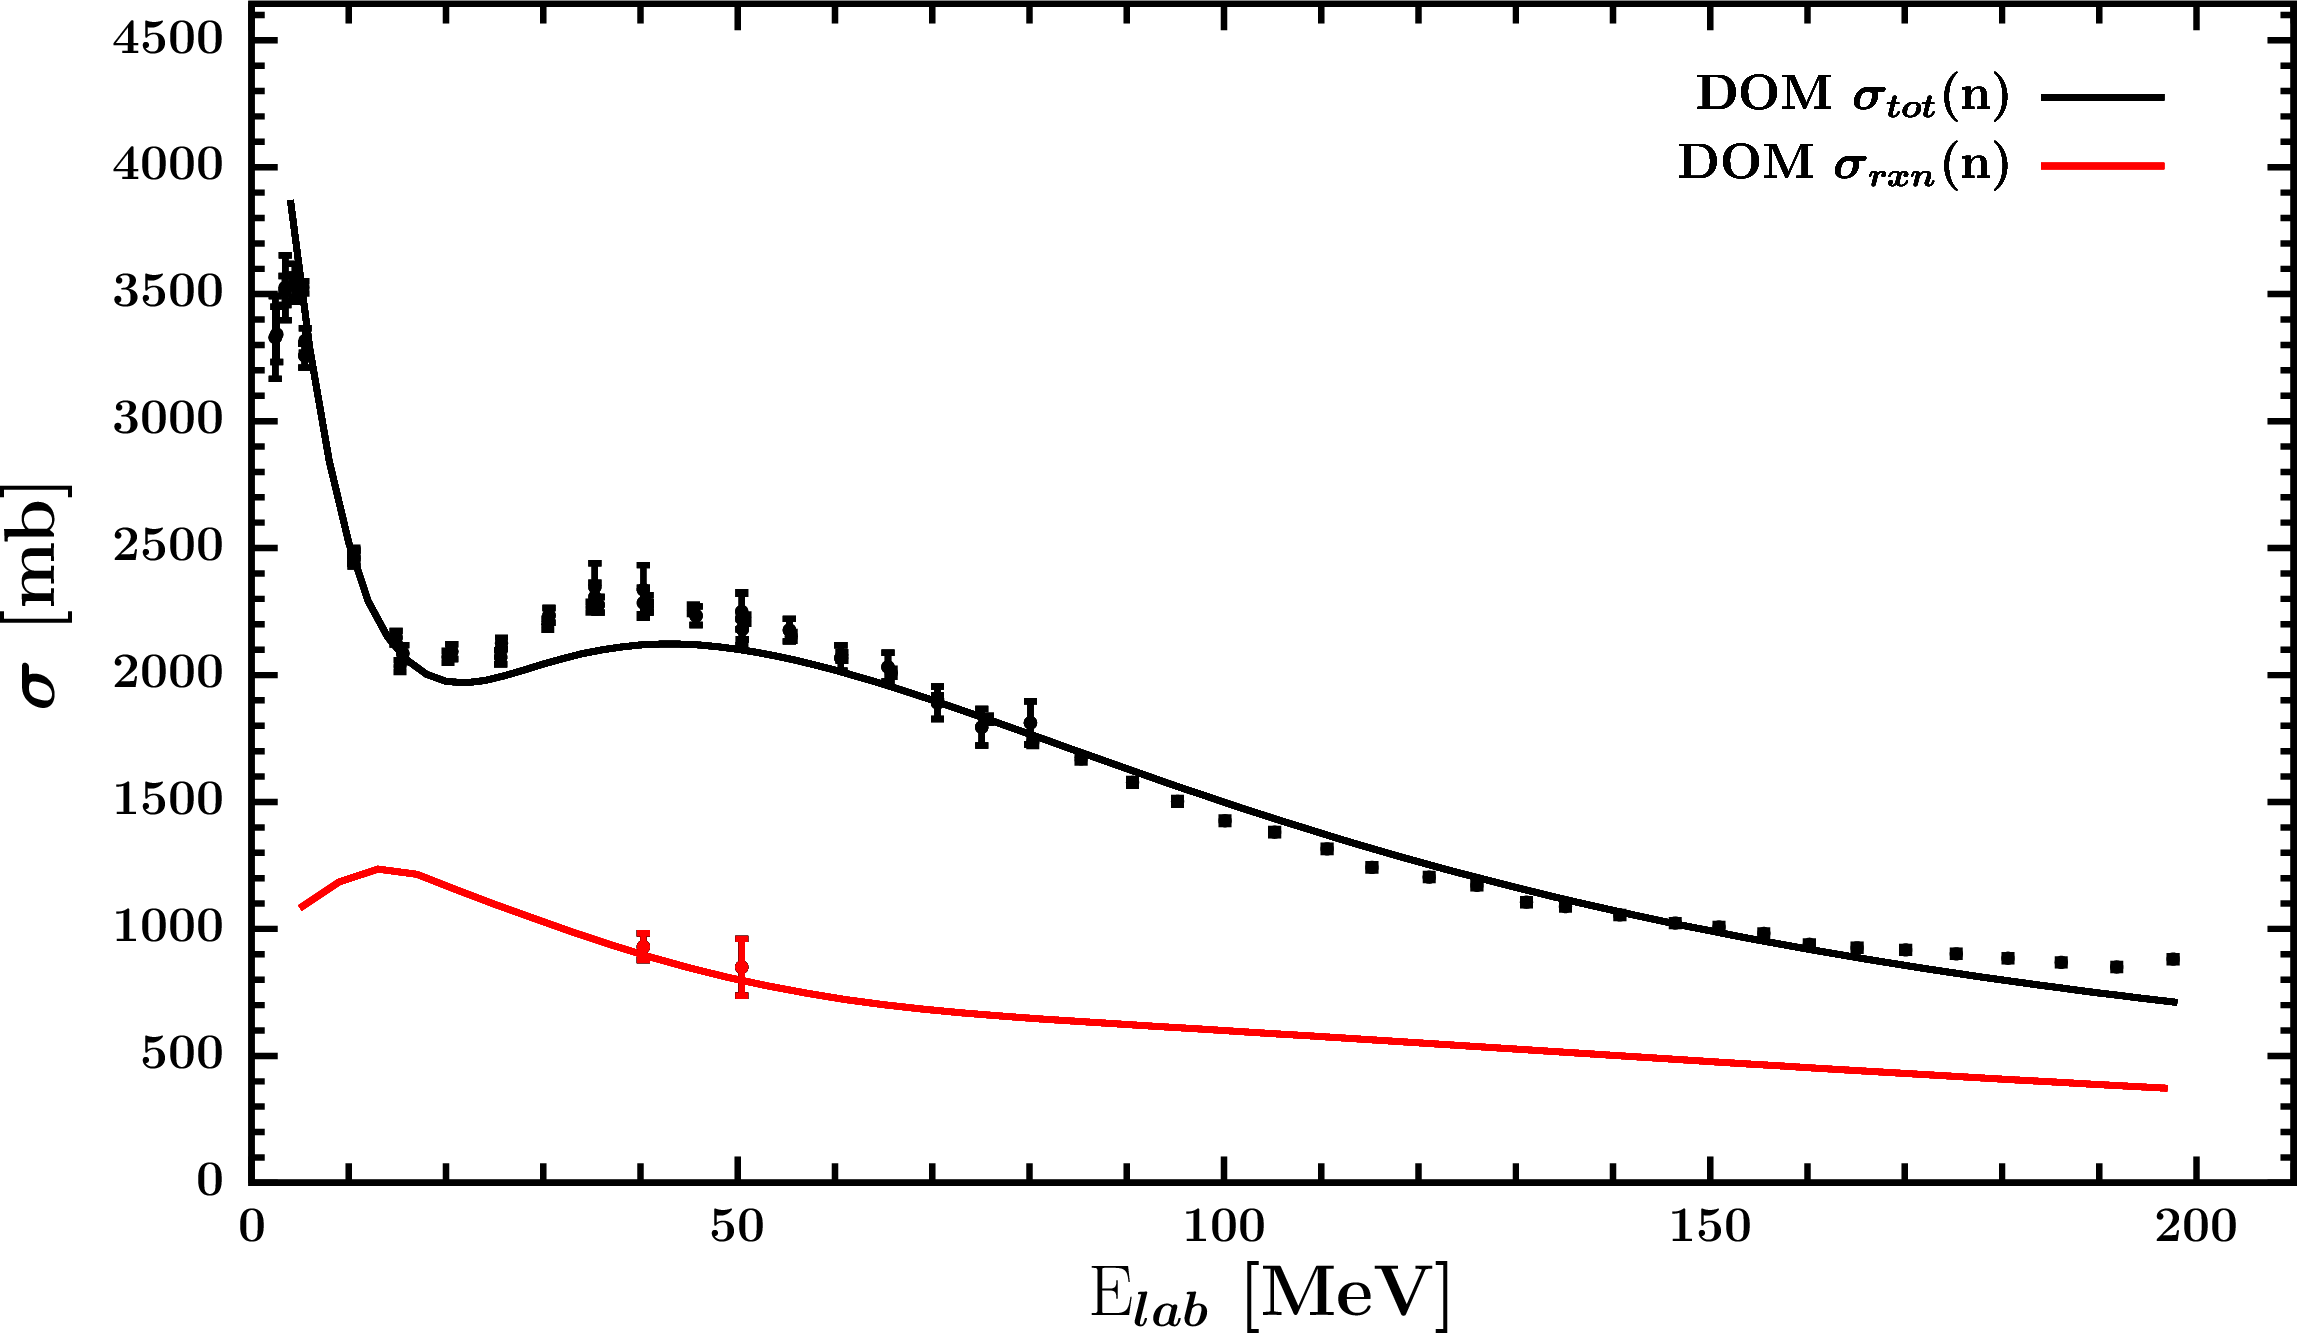
\includegraphics[width=1.0\textwidth]{figures/ca40_neutronInelastic.png}
        \caption{Neutron \rxn and \tot data}
        \label{DOMFitData_ca40_neutron_inelastic}
    \end{minipage}
\end{figure}

\afterpage{\clearpage}

\begin{figure}[H]
    \centering
    \begin{minipage}{0.45\textwidth}
        \centering
        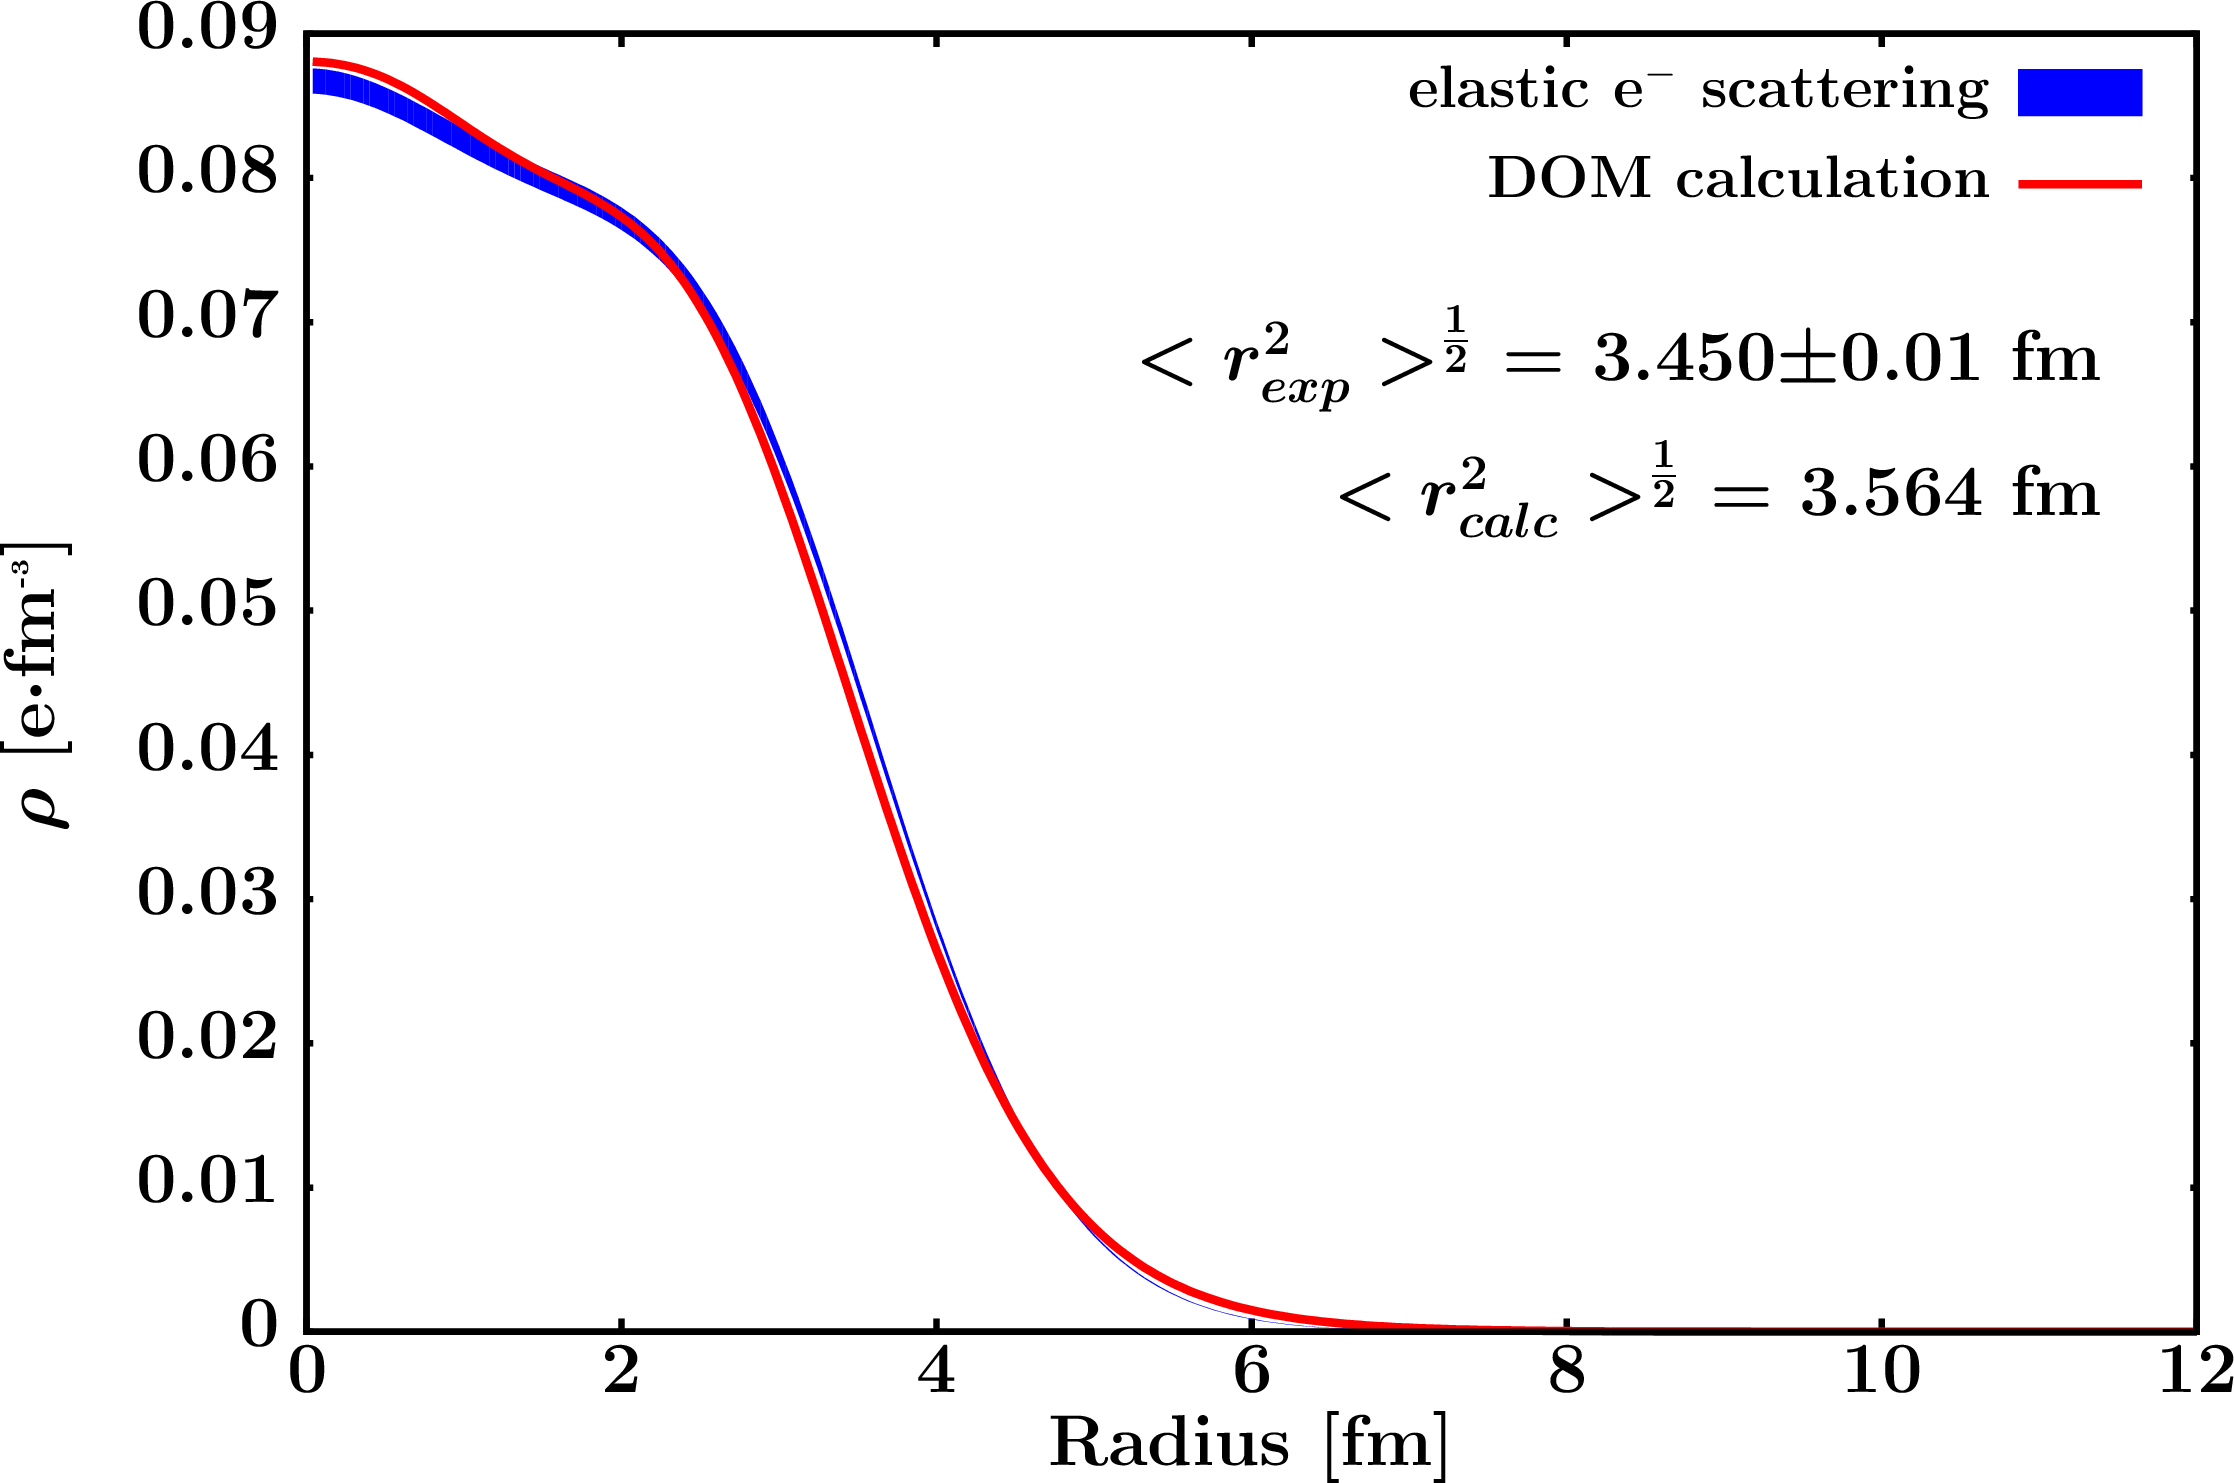
\includegraphics[width=1.0\textwidth]{figures/ca40_chargeDensity.png}
        \caption{Charge density data}
        \label{DOMFitData_ca40_chargeDensity}
    \end{minipage}\hfill
    \begin{minipage}{0.45\textwidth}
        \centering
        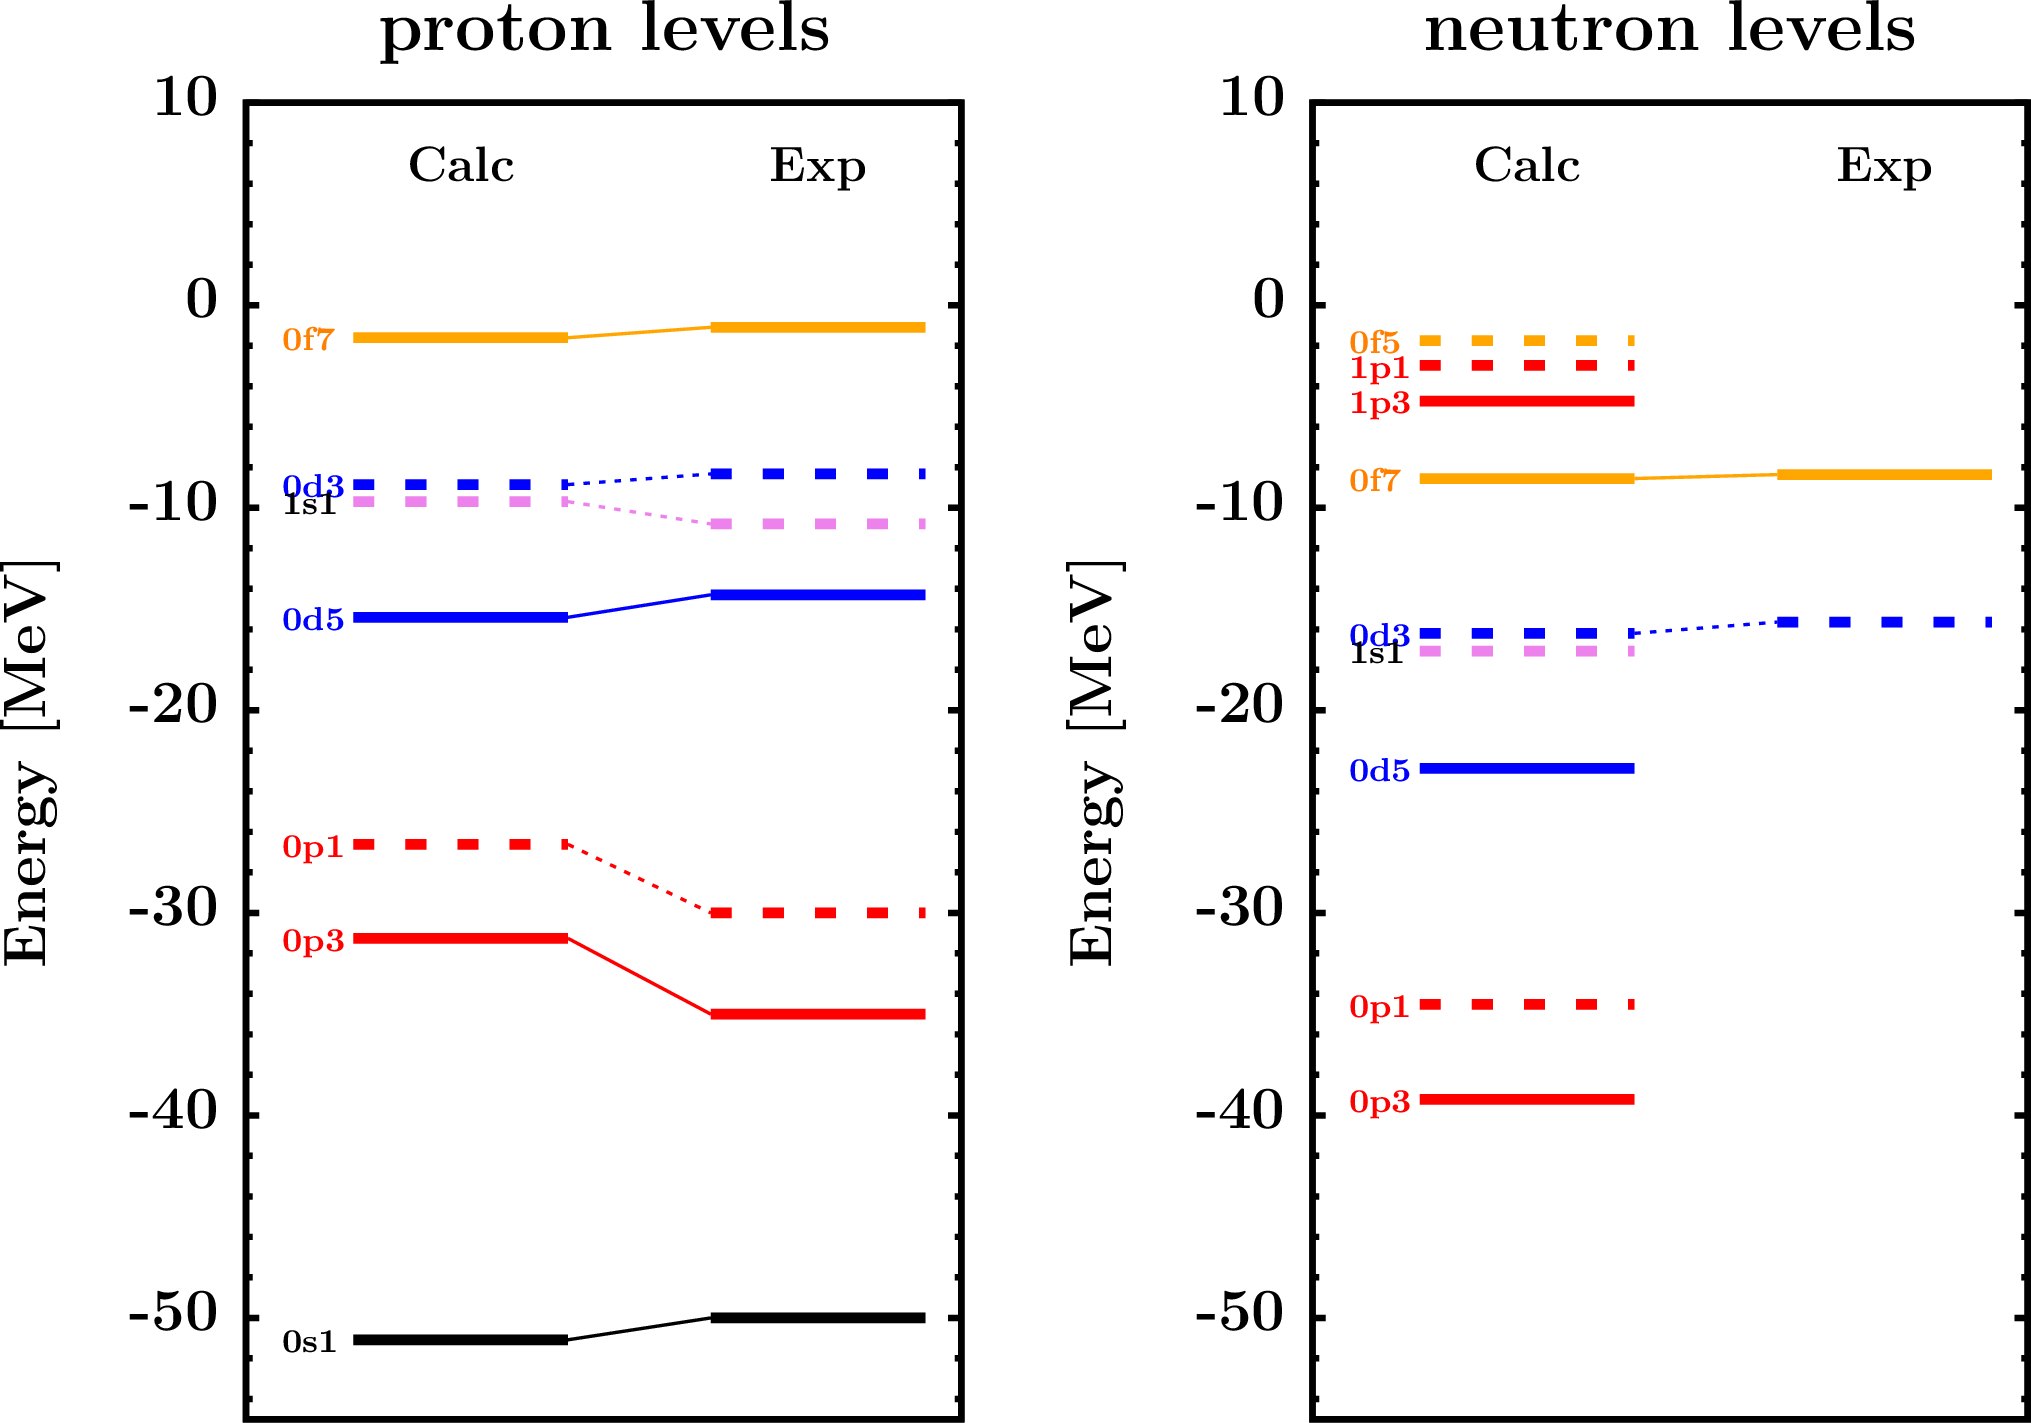
\includegraphics[width=1.0\textwidth]{figures/ca40_SPLevels.png}
        \caption{Single-particle levels}
        \label{DOMFitData_ca40_SPLevels}
    \end{minipage}
\end{figure}

\afterpage{\clearpage}

\begin{figure}[H]
    \centering
    \begin{minipage}{0.45\textwidth}
        \centering
        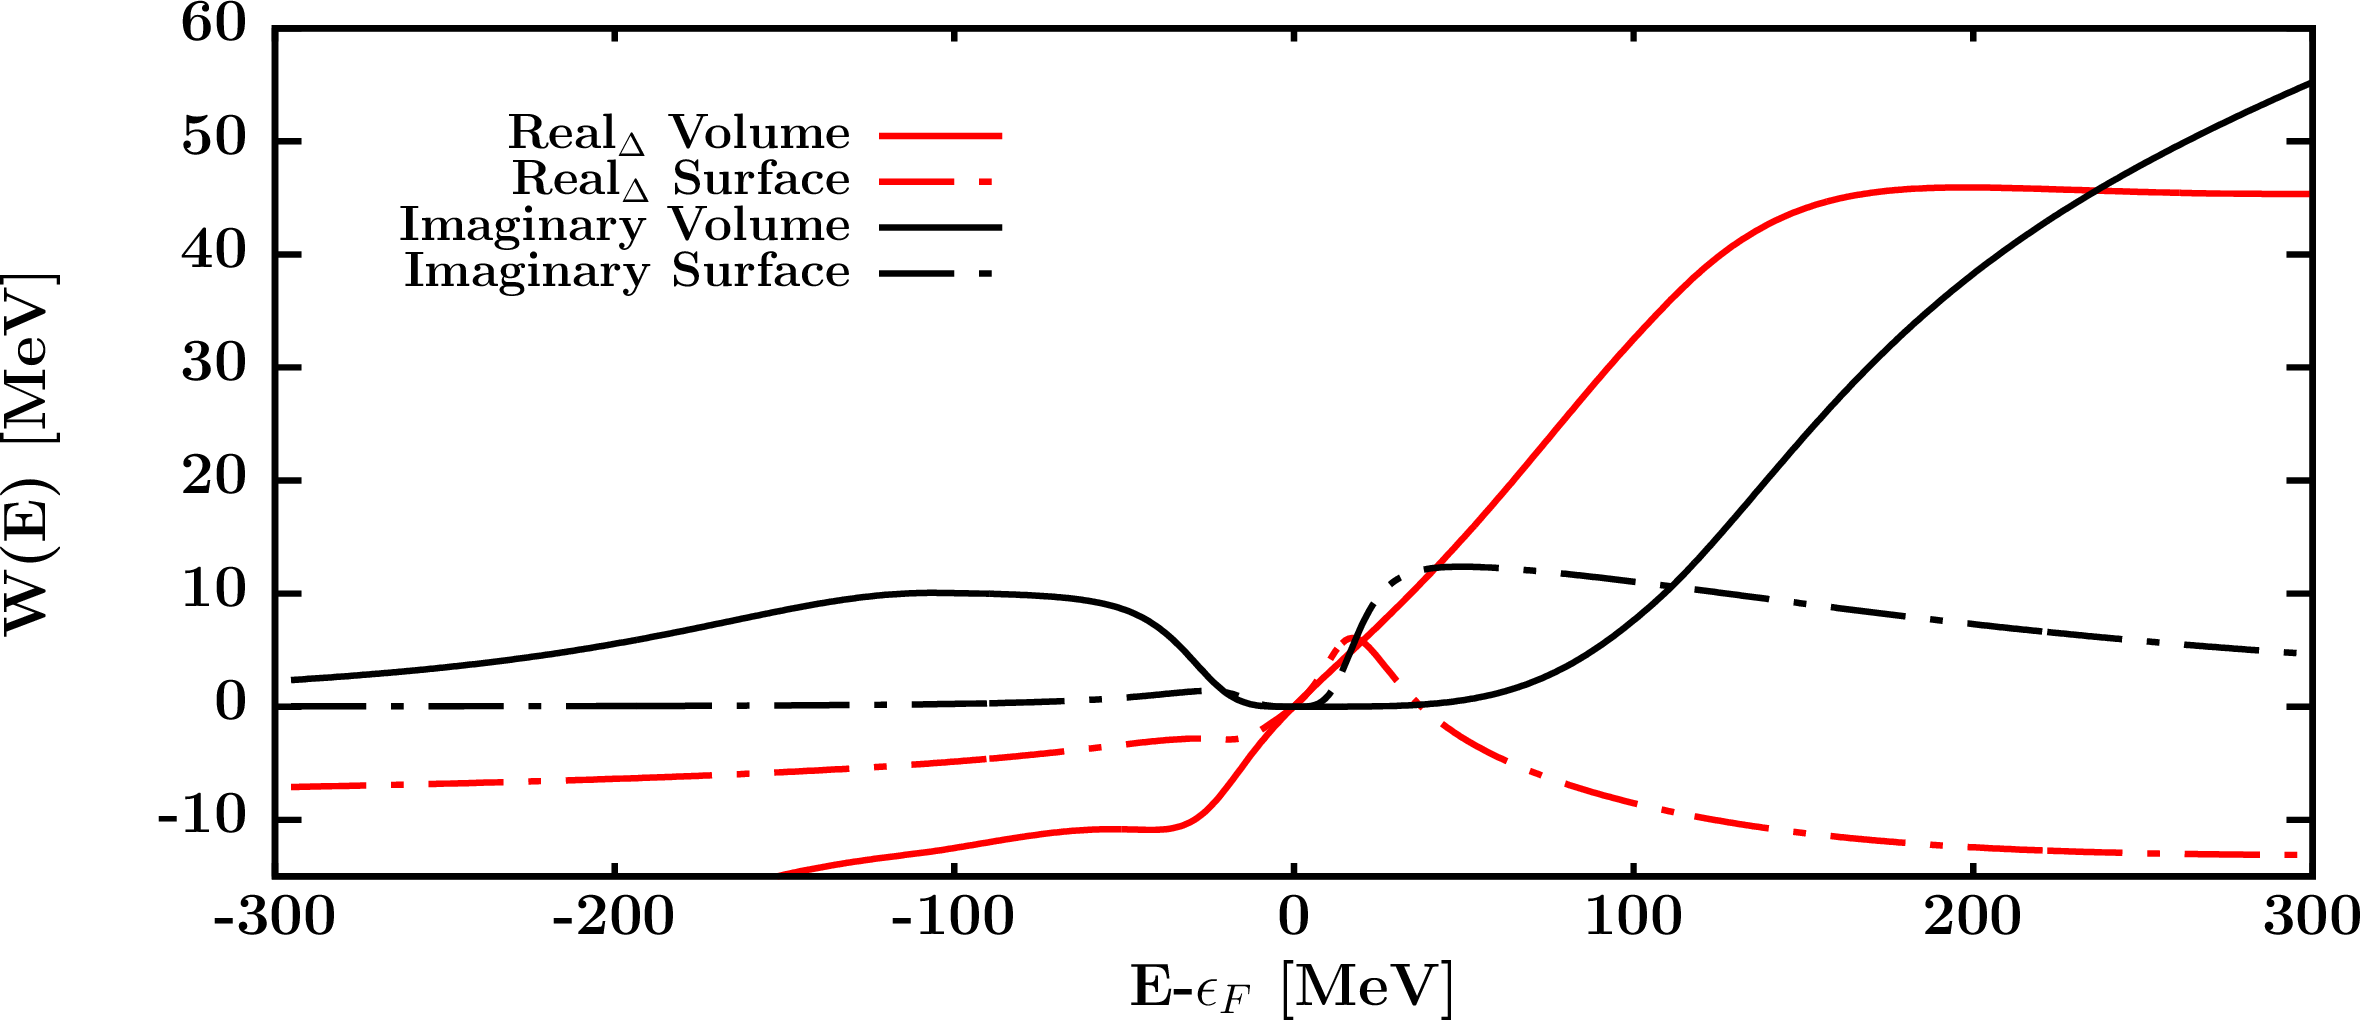
\includegraphics[width=1.0\textwidth]{figures/ca40_protonPotentials.png}
        \caption{Energy-dependence of optical potential components for protons
        on \caForty}
        \label{DOMFitData_ca40_proton_potentialComponent_energy}
    \end{minipage}\hfill
    \begin{minipage}{0.45\textwidth}
        \centering
        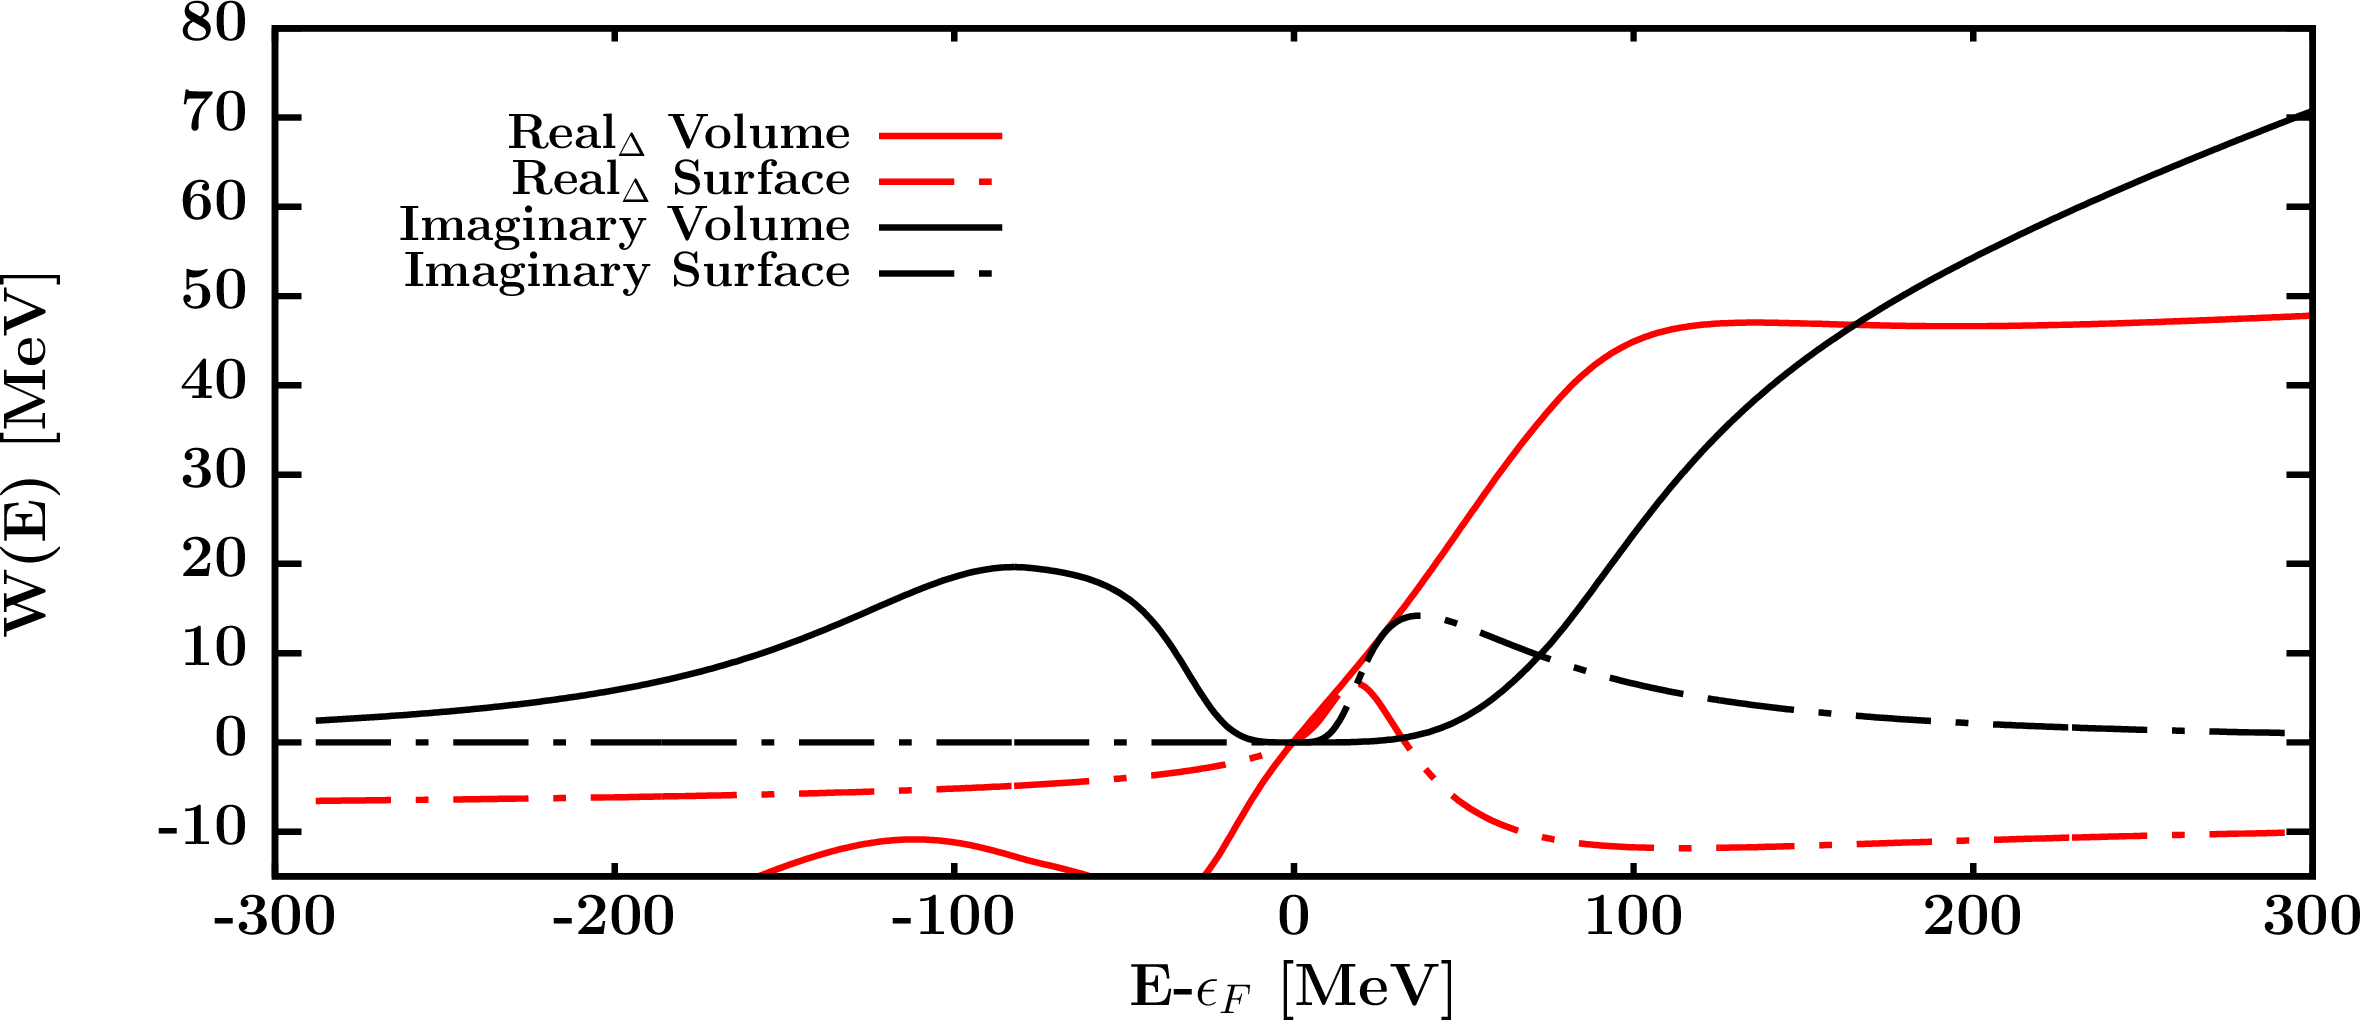
\includegraphics[width=1.0\textwidth]{figures/ca40_neutronPotentials.png}
        \caption{Neutron potential energy-dependent component}
        \label{DOMFitData_ca40_neutron_potentialComponent_energy}
    \end{minipage}
\end{figure}

\begin{figure}[H]
    \centering
    \begin{minipage}{0.45\textwidth}
        \centering
        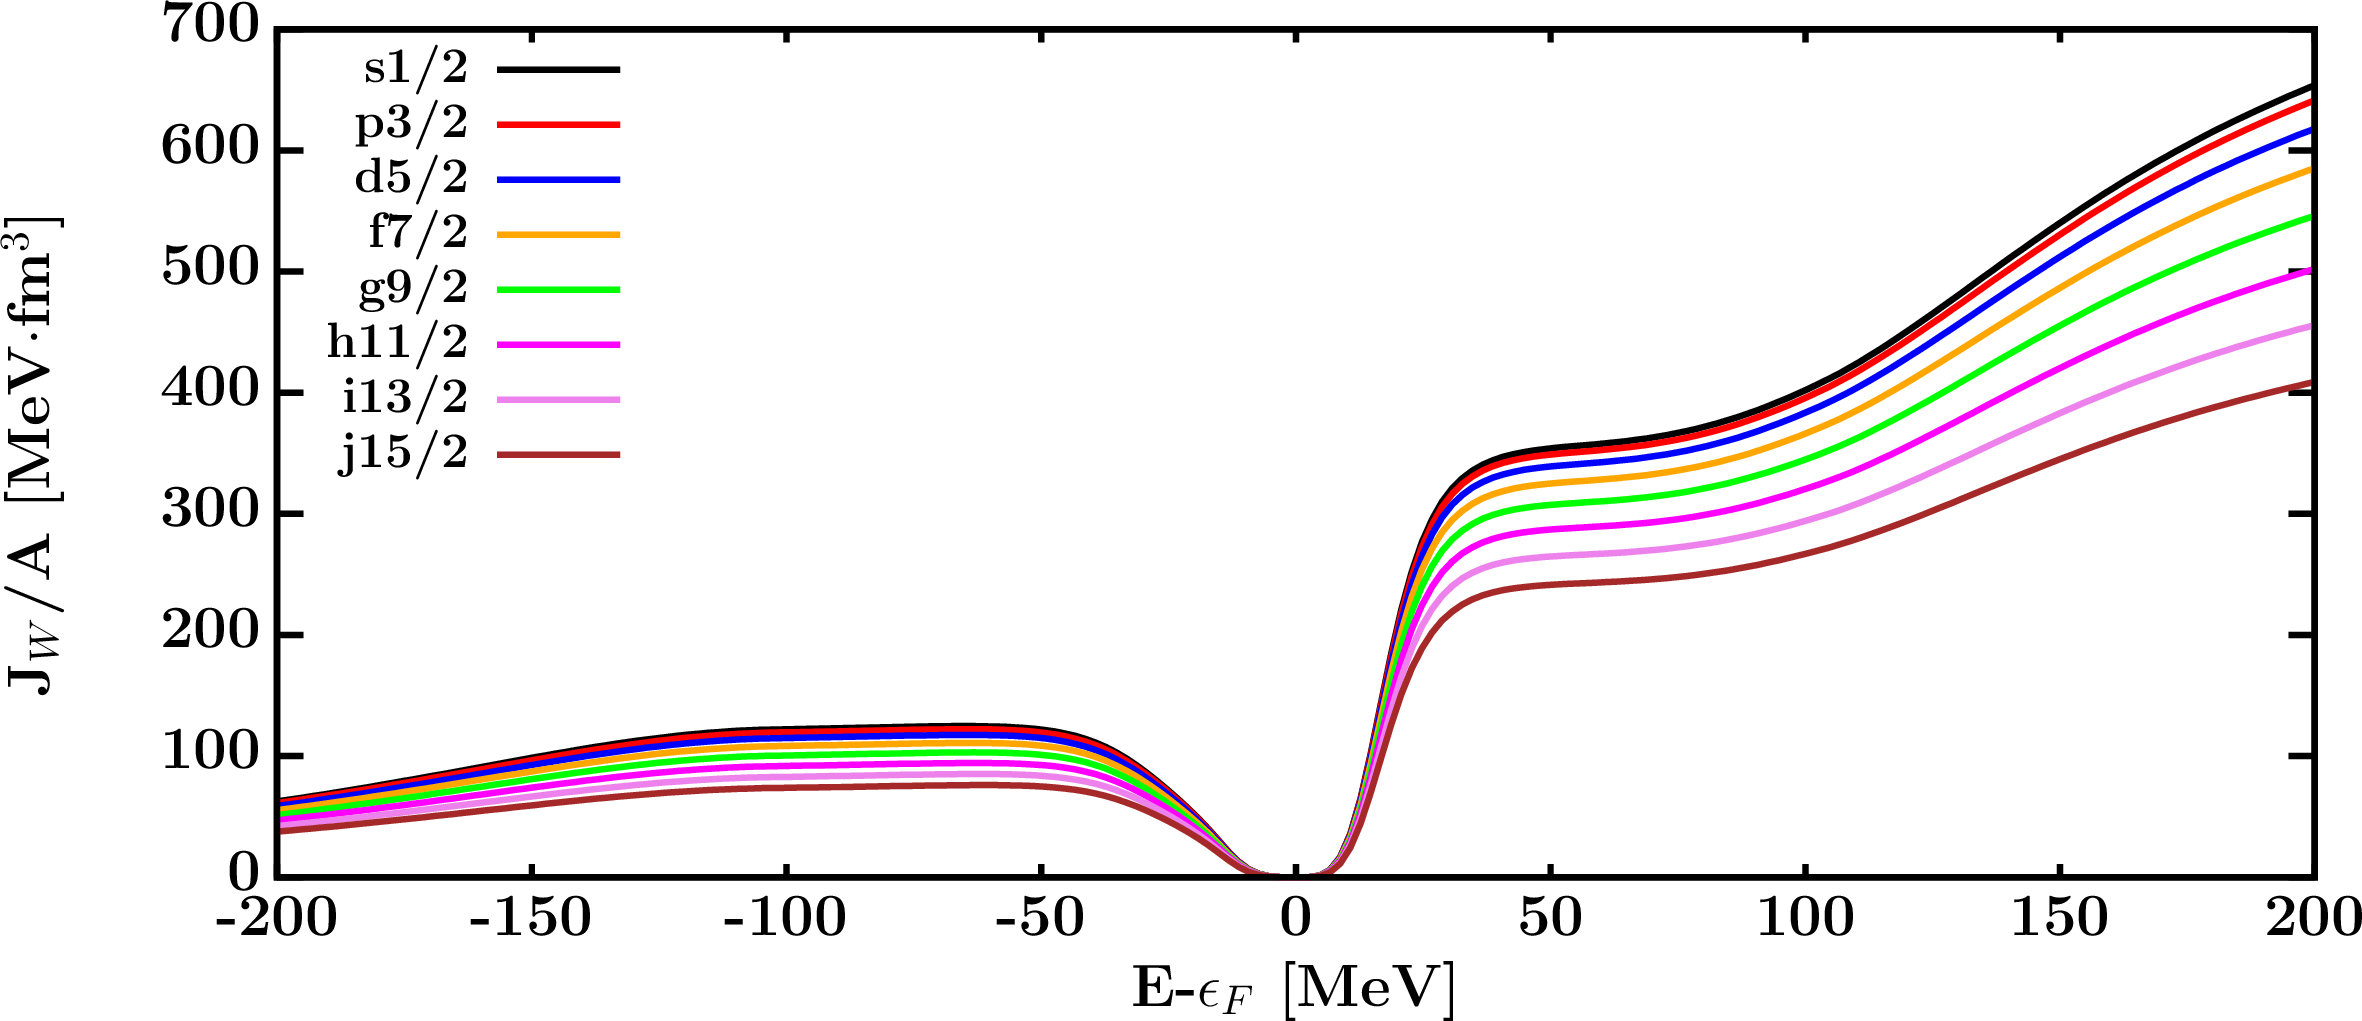
\includegraphics[width=1.0\textwidth]{figures/ca40_protonVolumeIntegrals.png}
        \caption{Proton potential, integrated over r-space}
        \label{DOMFitData_ca40_proton_potentialIntegral}
    \end{minipage}\hfill
    \begin{minipage}{0.45\textwidth}
        \centering
        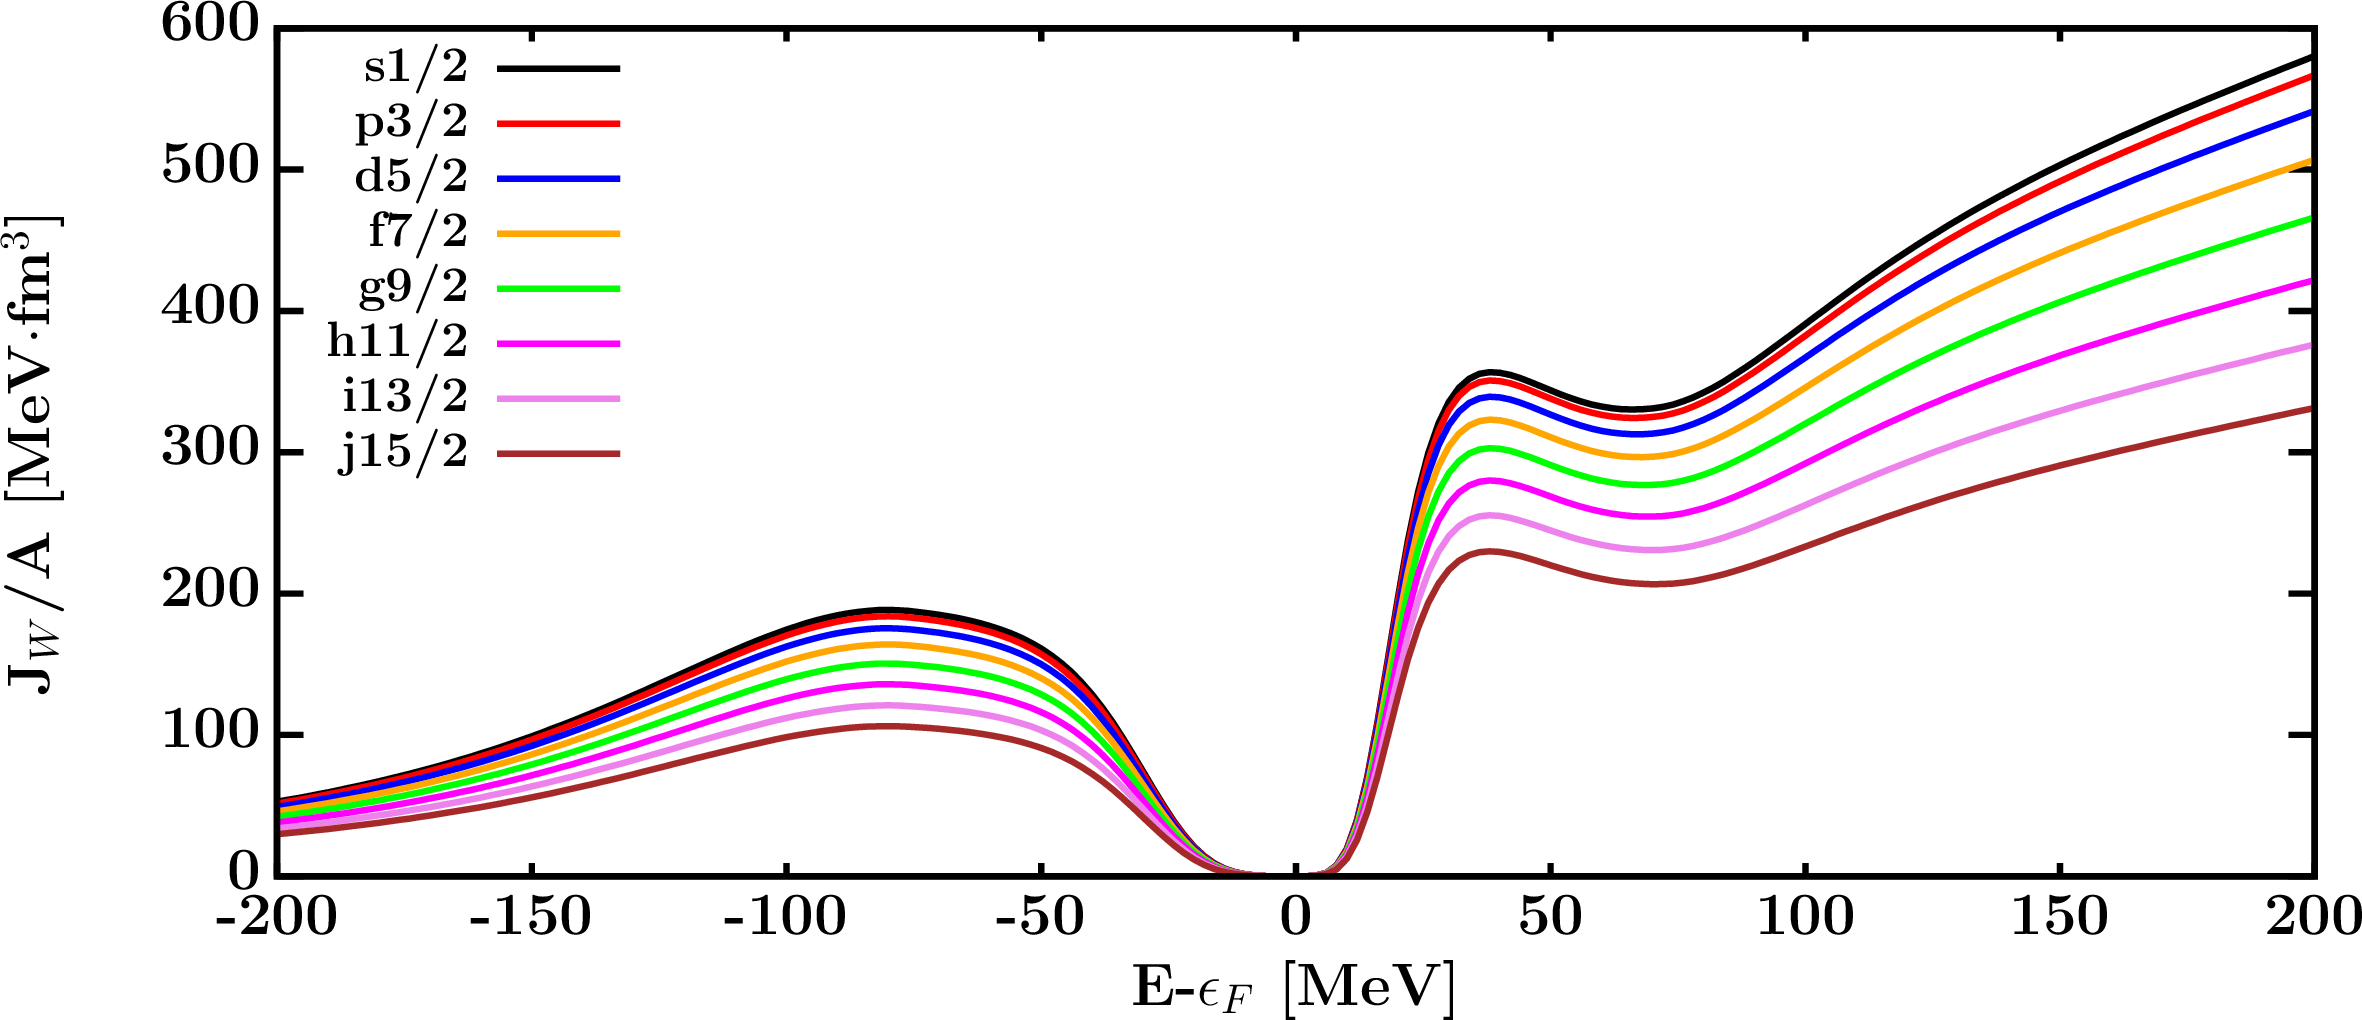
\includegraphics[width=1.0\textwidth]{figures/ca40_neutronVolumeIntegrals.png}
        \caption{Neutron potential, integrated over r-space}
        \label{DOMFitData_ca40_neutron_potentialIntegral}
    \end{minipage}
\end{figure}

\afterpage{\clearpage}

\begin{figure}[H]
    \centering
    \begin{minipage}{0.45\textwidth}
        \centering
        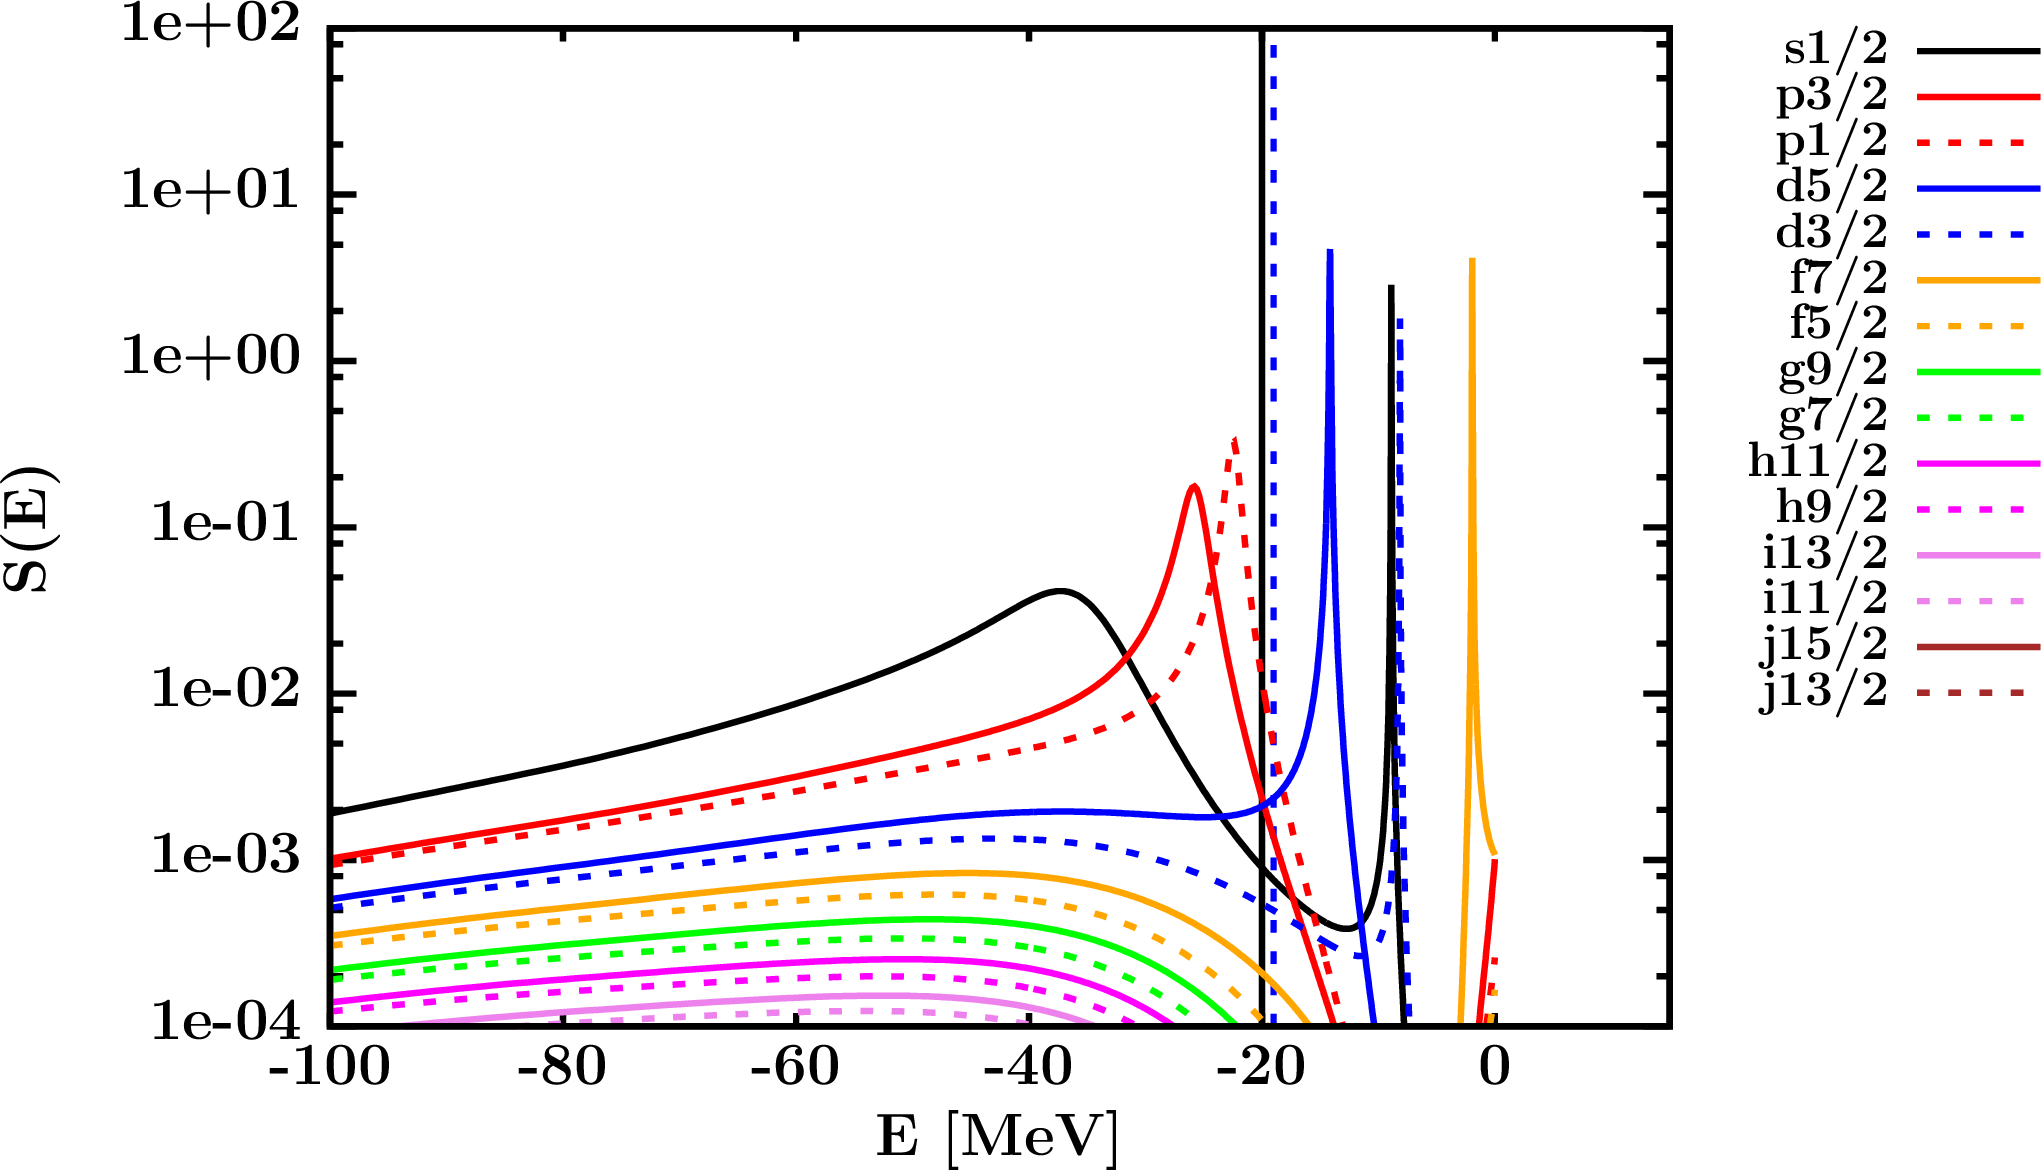
\includegraphics[width=1.0\textwidth]{figures/ca40_protonSpectralFunctions.png}
        \caption{Proton spectral functions}
        \label{DOMFitData_ca40_proton_spectralFunctions}
    \end{minipage}\hfill
    \begin{minipage}{0.45\textwidth}
        \centering
        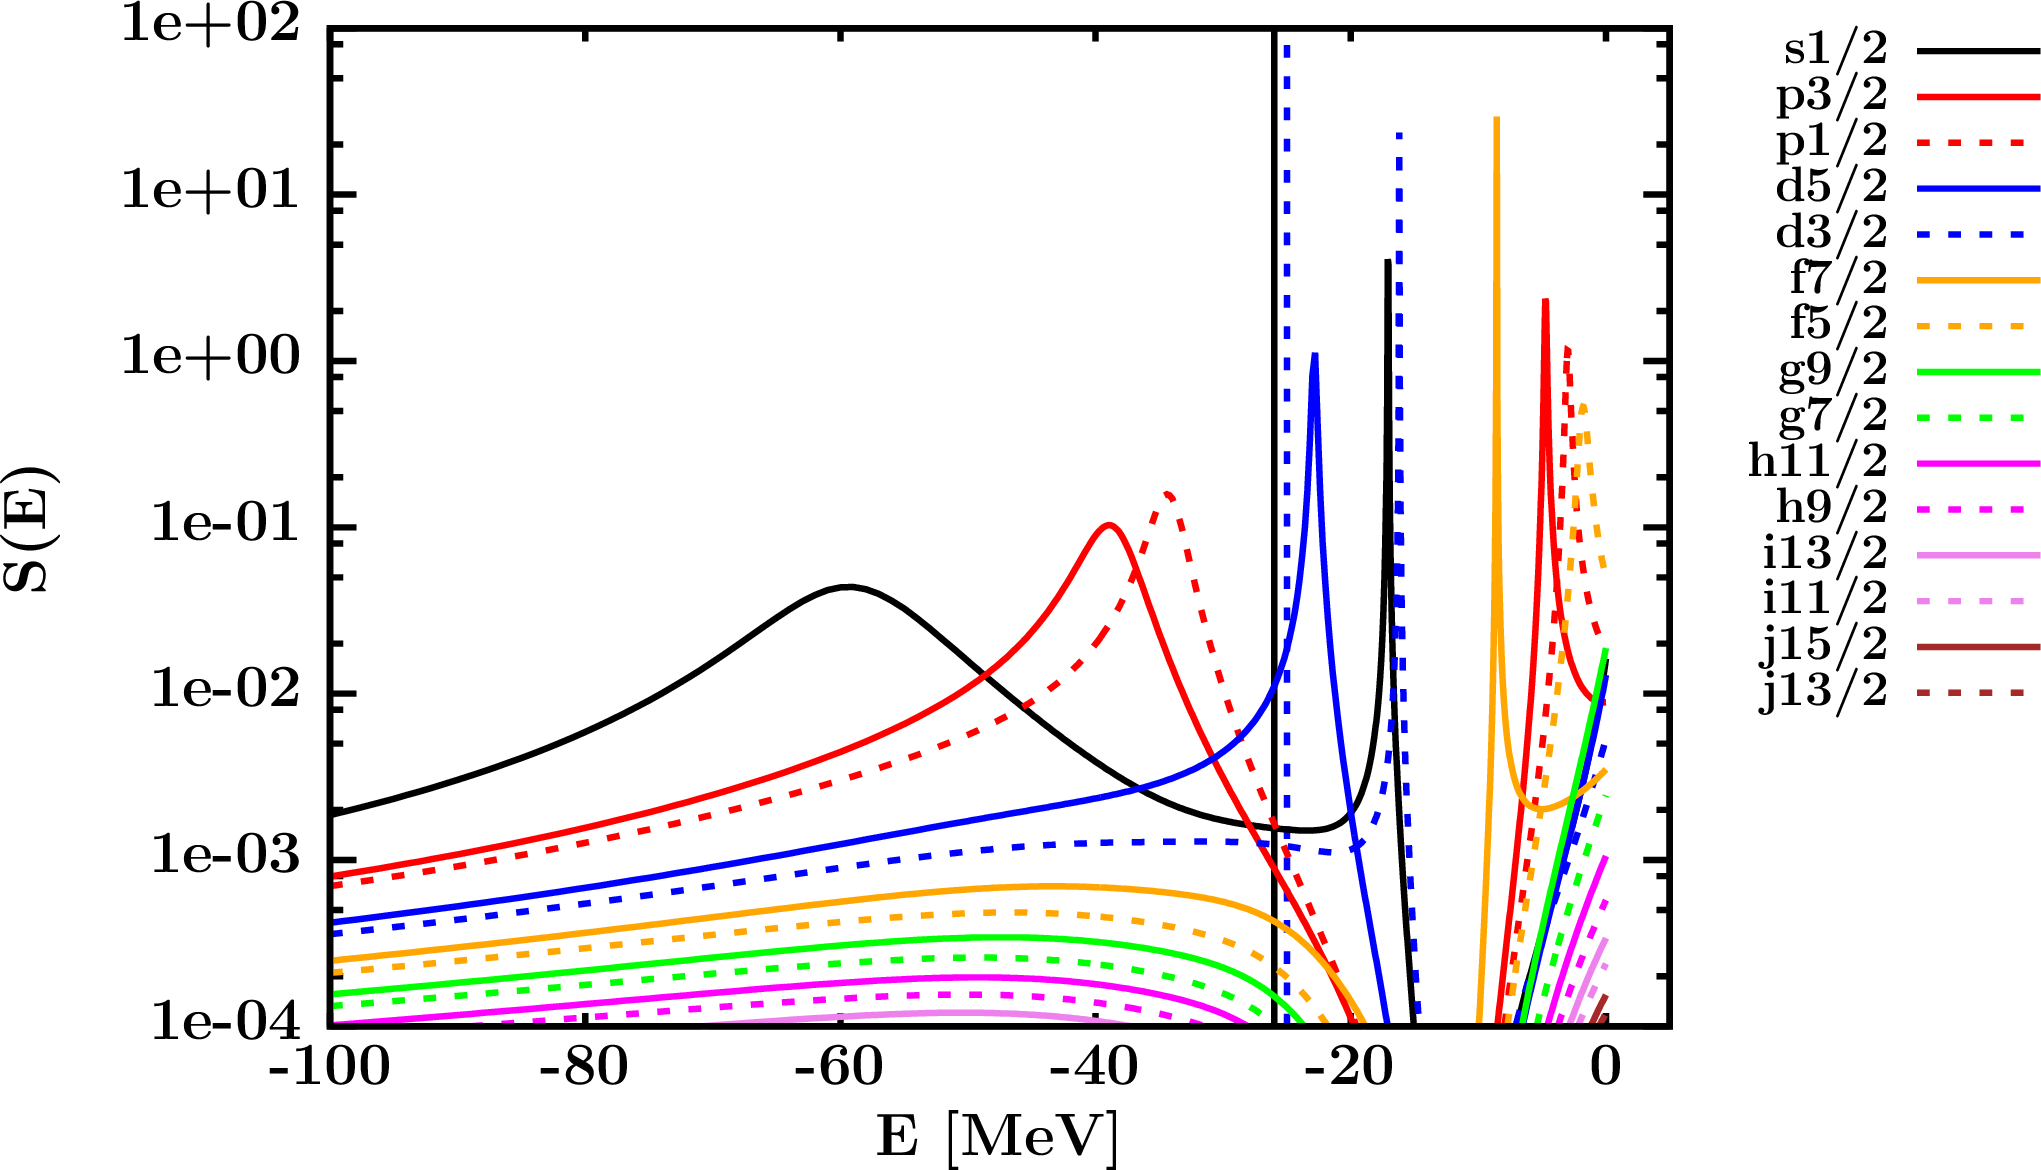
\includegraphics[width=1.0\textwidth]{figures/ca40_neutronSpectralFunctions.png}
        \caption{Neutron spectral functions}
        \label{DOMFitData_ca40_neutron_spectralFunctions}
    \end{minipage}
\end{figure}

\begin{figure}[H]
    \centering
    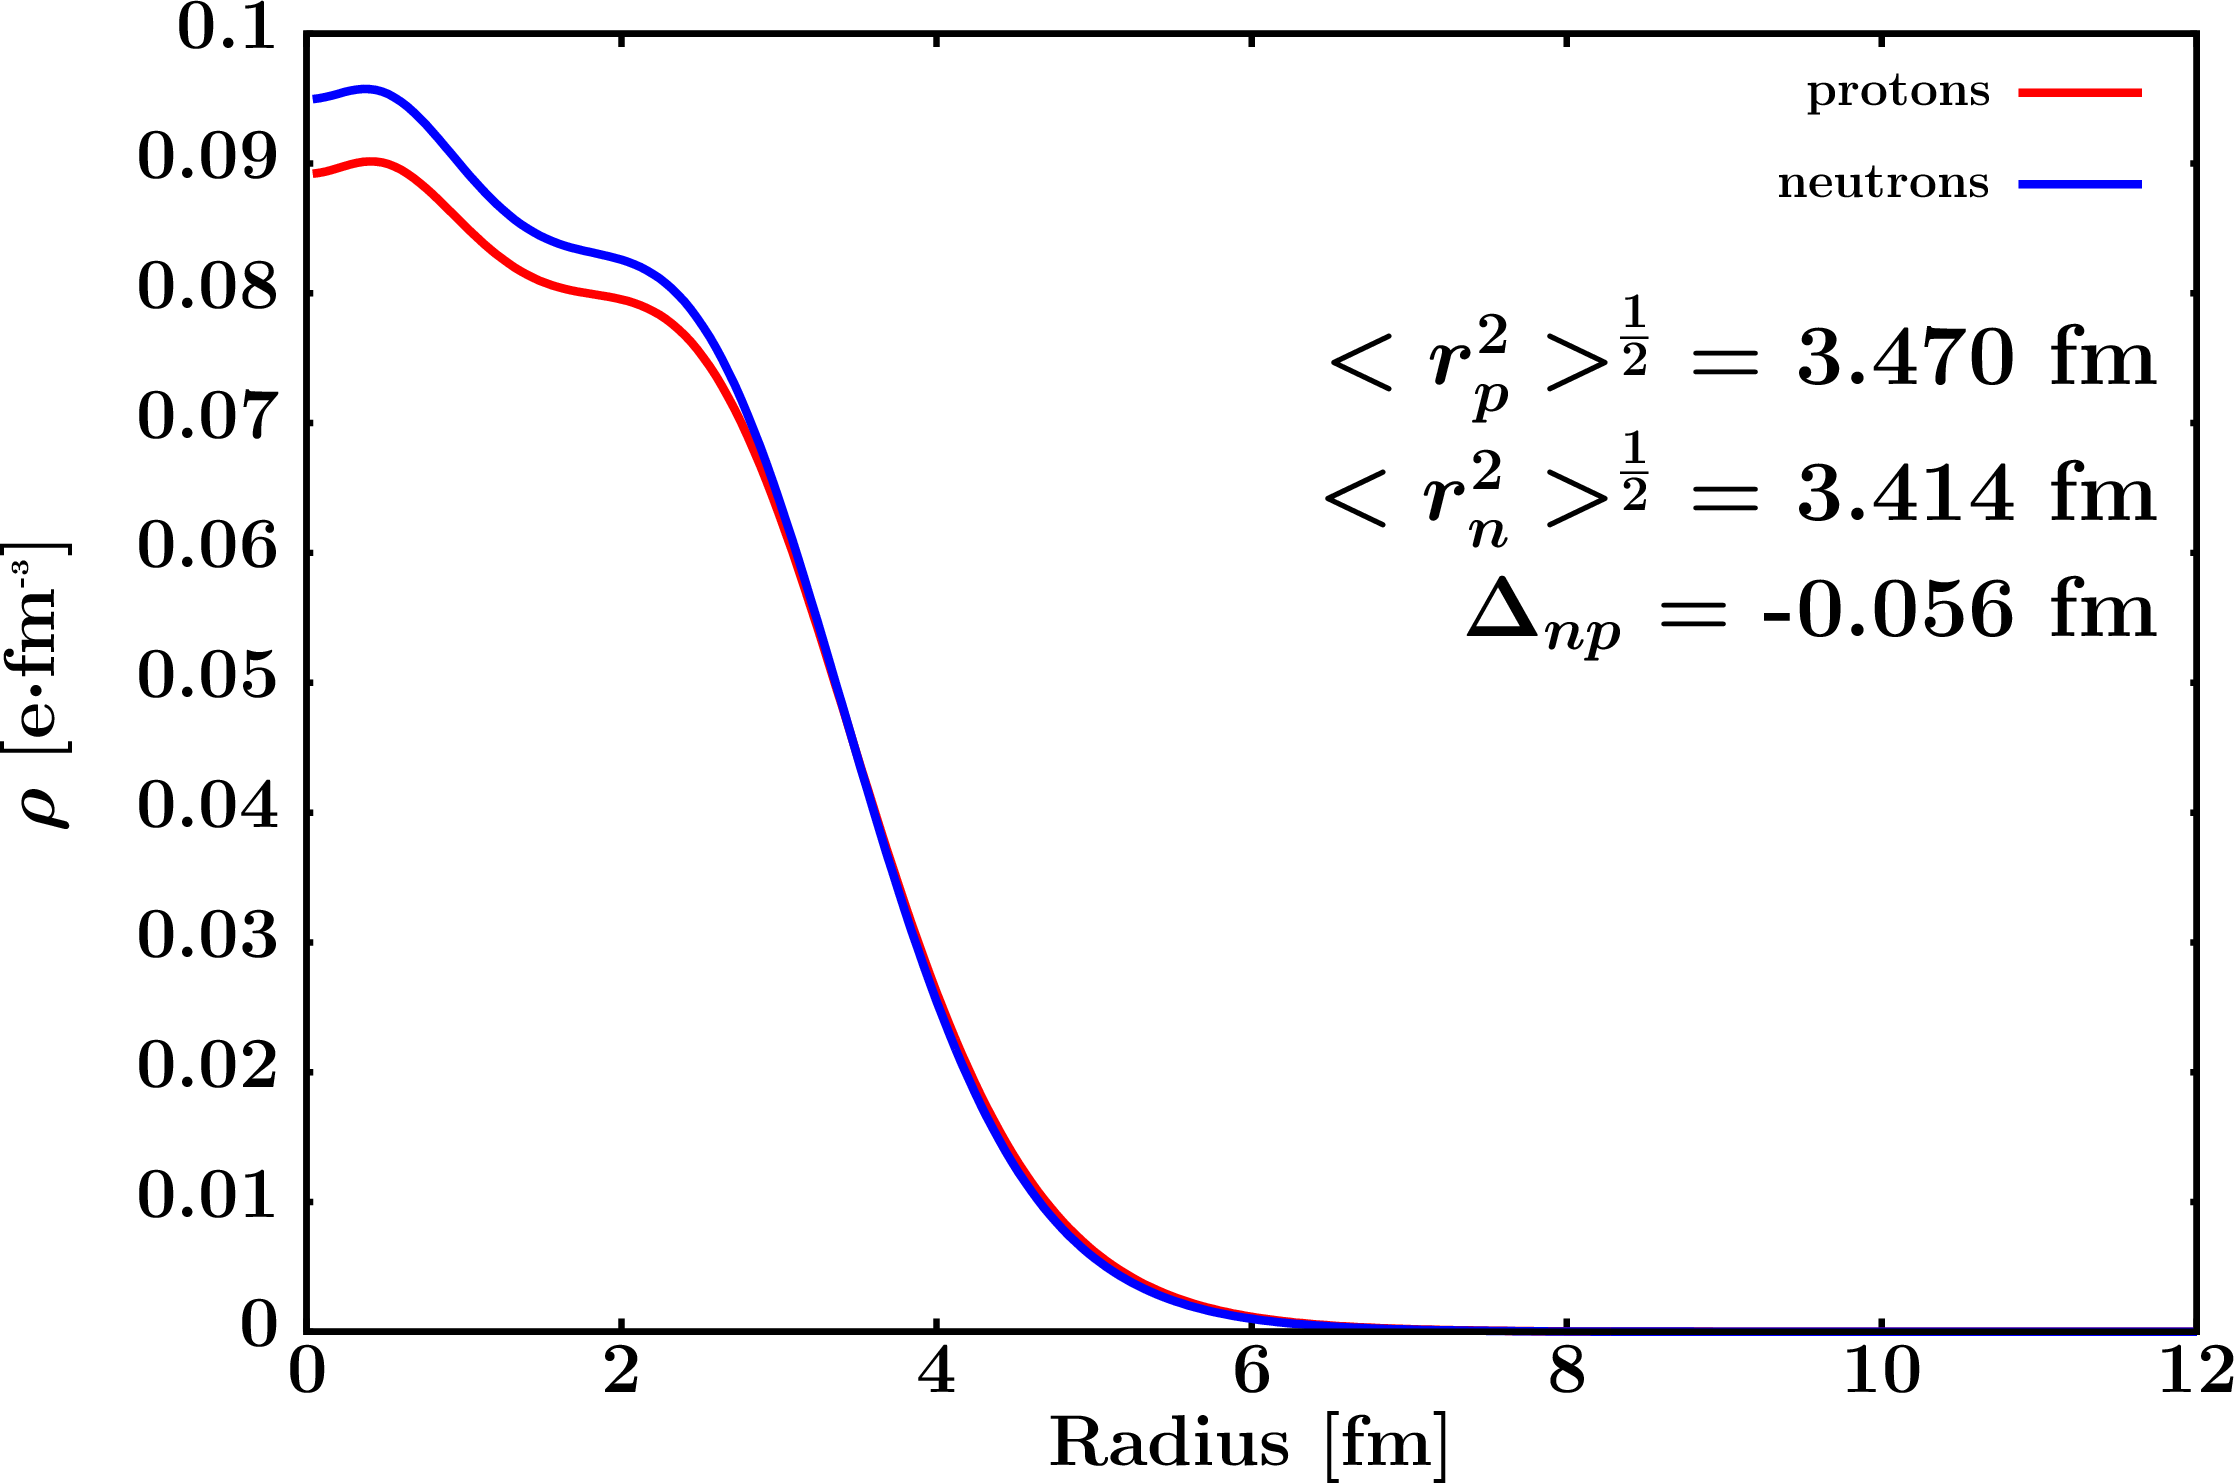
\includegraphics[width = 0.5\textwidth]{figures/ca40_matterDensity.png}
    \caption{Matter density distribution}
    \label{DOMFitData_ca40_matterDensity}
\end{figure}

\begin{figure}[H]
    \centering
    \includegraphics[width = 0.5\textwidth]{figures/ca40_momentumDistribution.png}
    \caption{Momentum distribution}
    \label{DOMFitData_ca40_momentumDistribution}
\end{figure}

\begin{figure}[H]
    \centering
    \includegraphics[width = 0.5\textwidth]{figures/ca40_energyDensity.png}
    \caption{Energy density distribution}
    \label{DOMFitData_ca40_energyDensity}
\end{figure}

\begin{figure}[H]
    \centering
    \includegraphics[width = 1.0\textwidth]{figures/ca40_eep.png}
    \caption{(e,e'p) cross sections}
    \label{DOMFitData_ca40_eep}
\end{figure}


\section{DOM fit of \caEight}

\label{ca48DOMOutput}
\begin{figure}[H]
    \centering
    \begin{minipage}{0.45\textwidth}
        \centering
        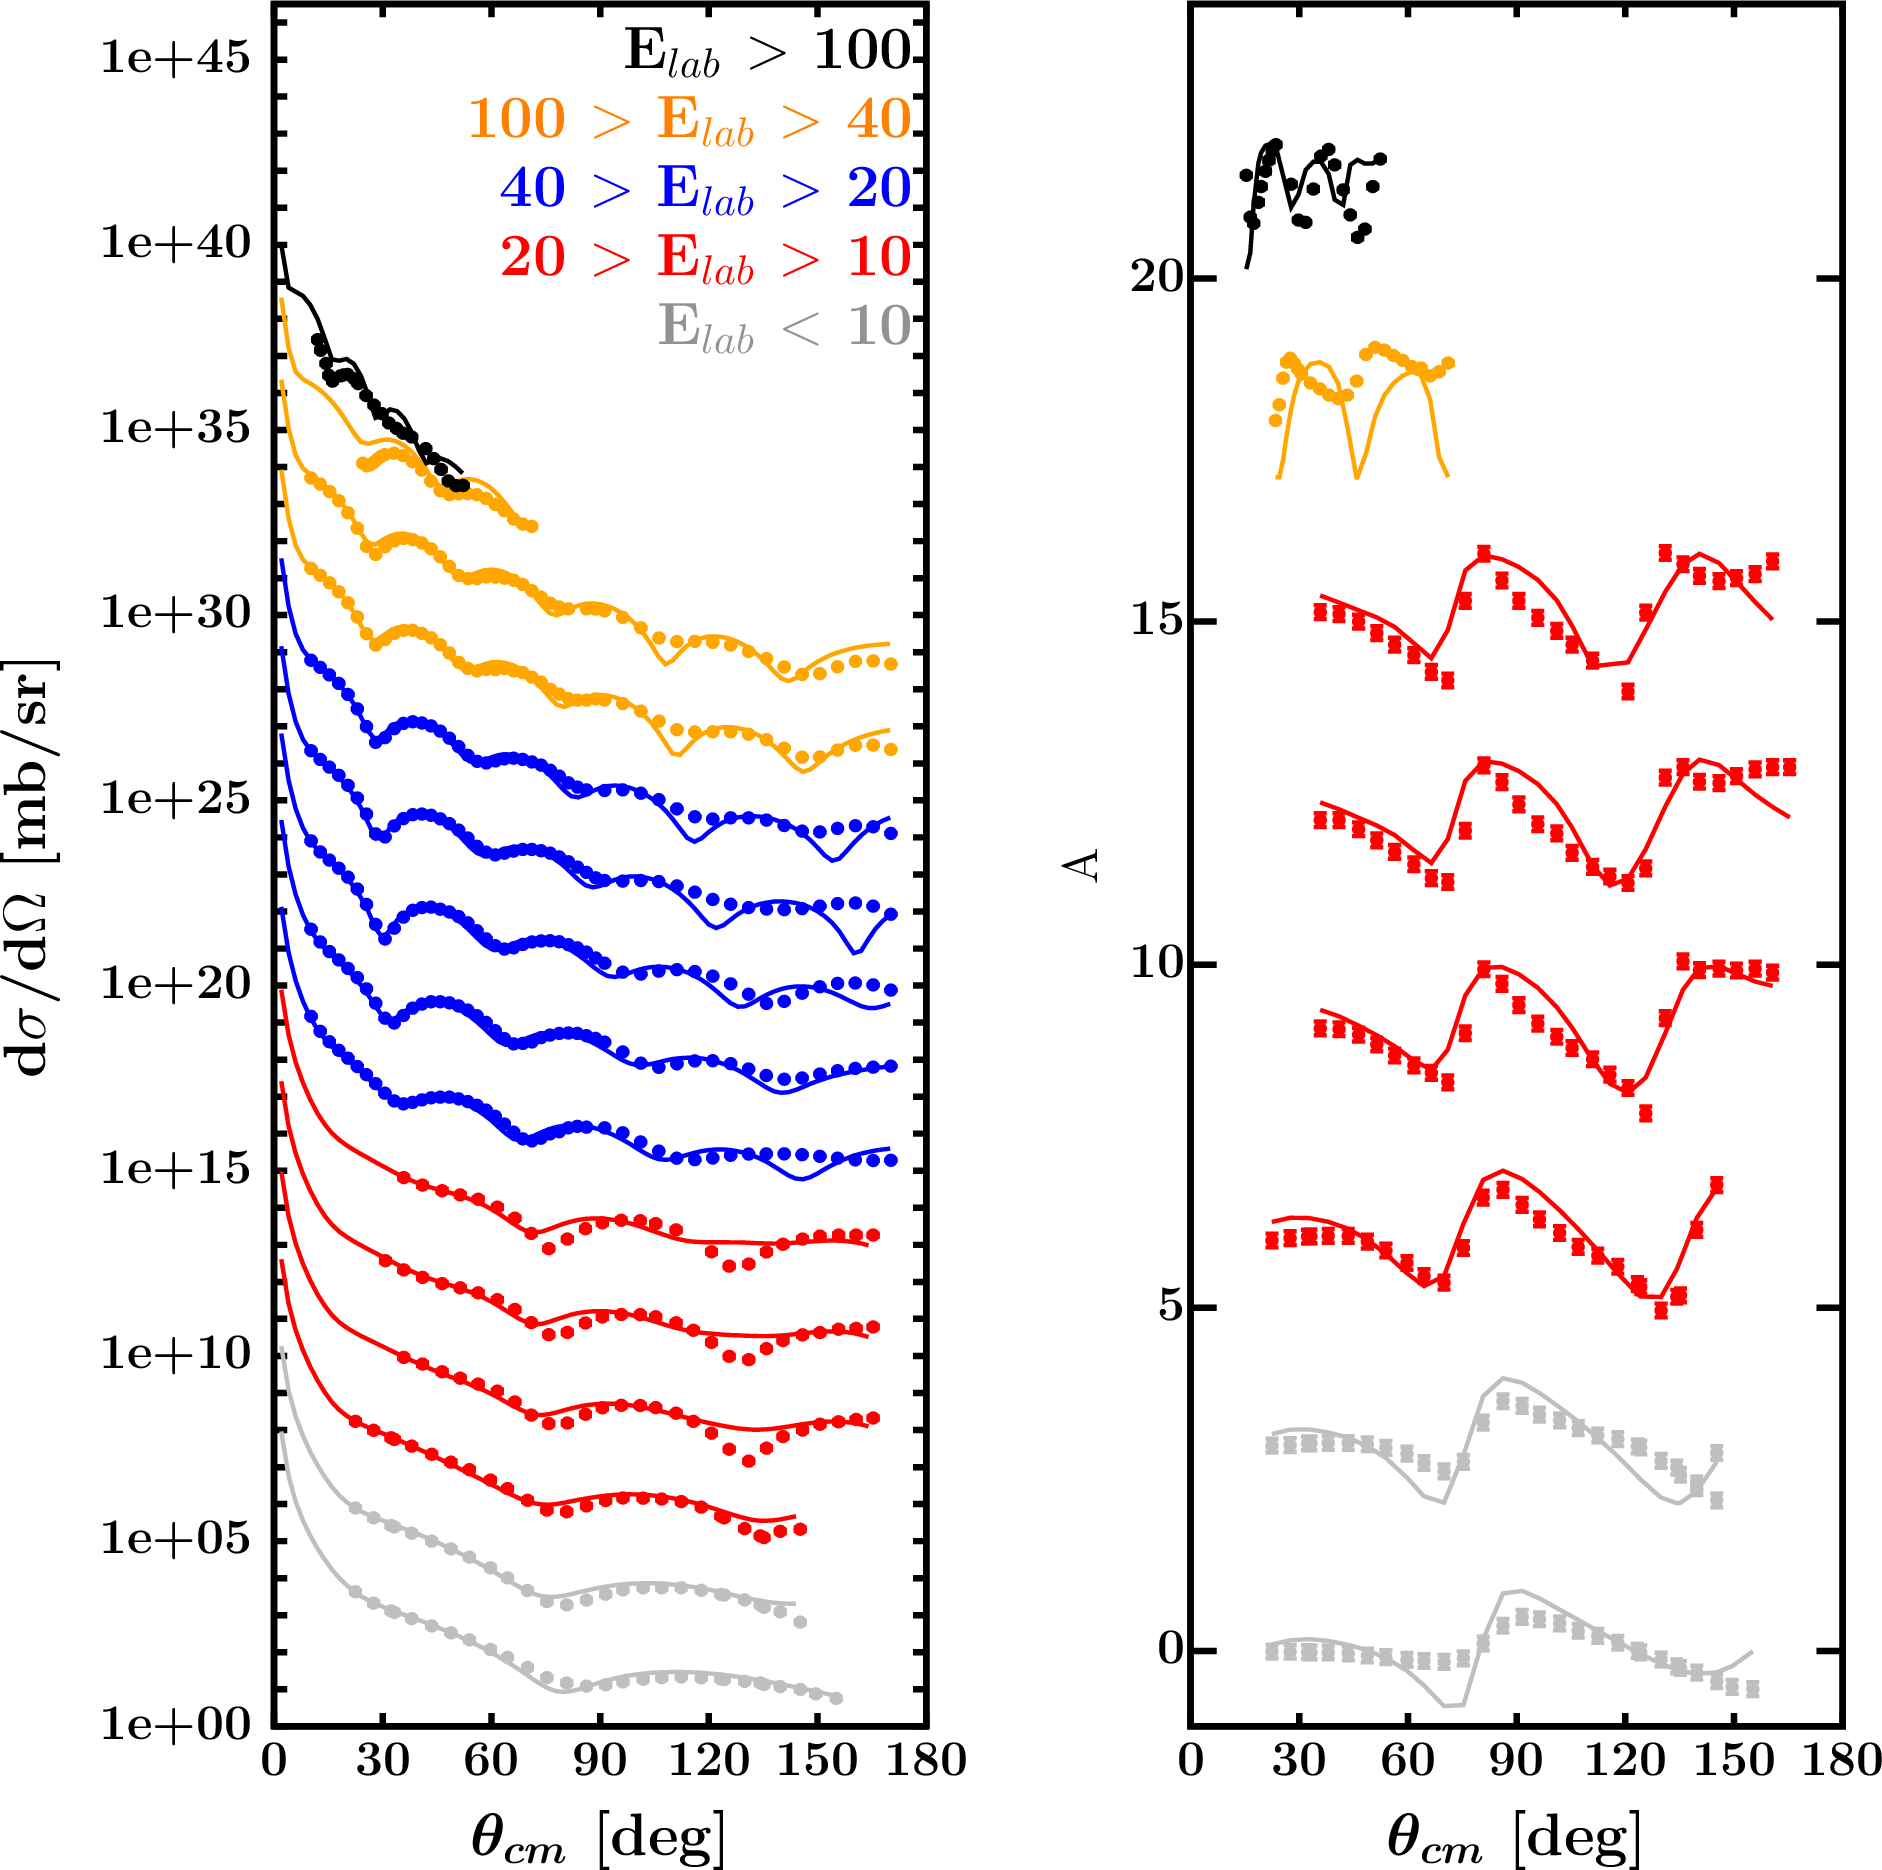
\includegraphics[width=1.0\textwidth]{figures/ca48_protonElastic.png}
        \caption{Proton elastic scattering data}
        \label{DOMFitData_ca48_proton_elastic}
    \end{minipage}\hfill
    \begin{minipage}{0.45\textwidth}
        \centering
        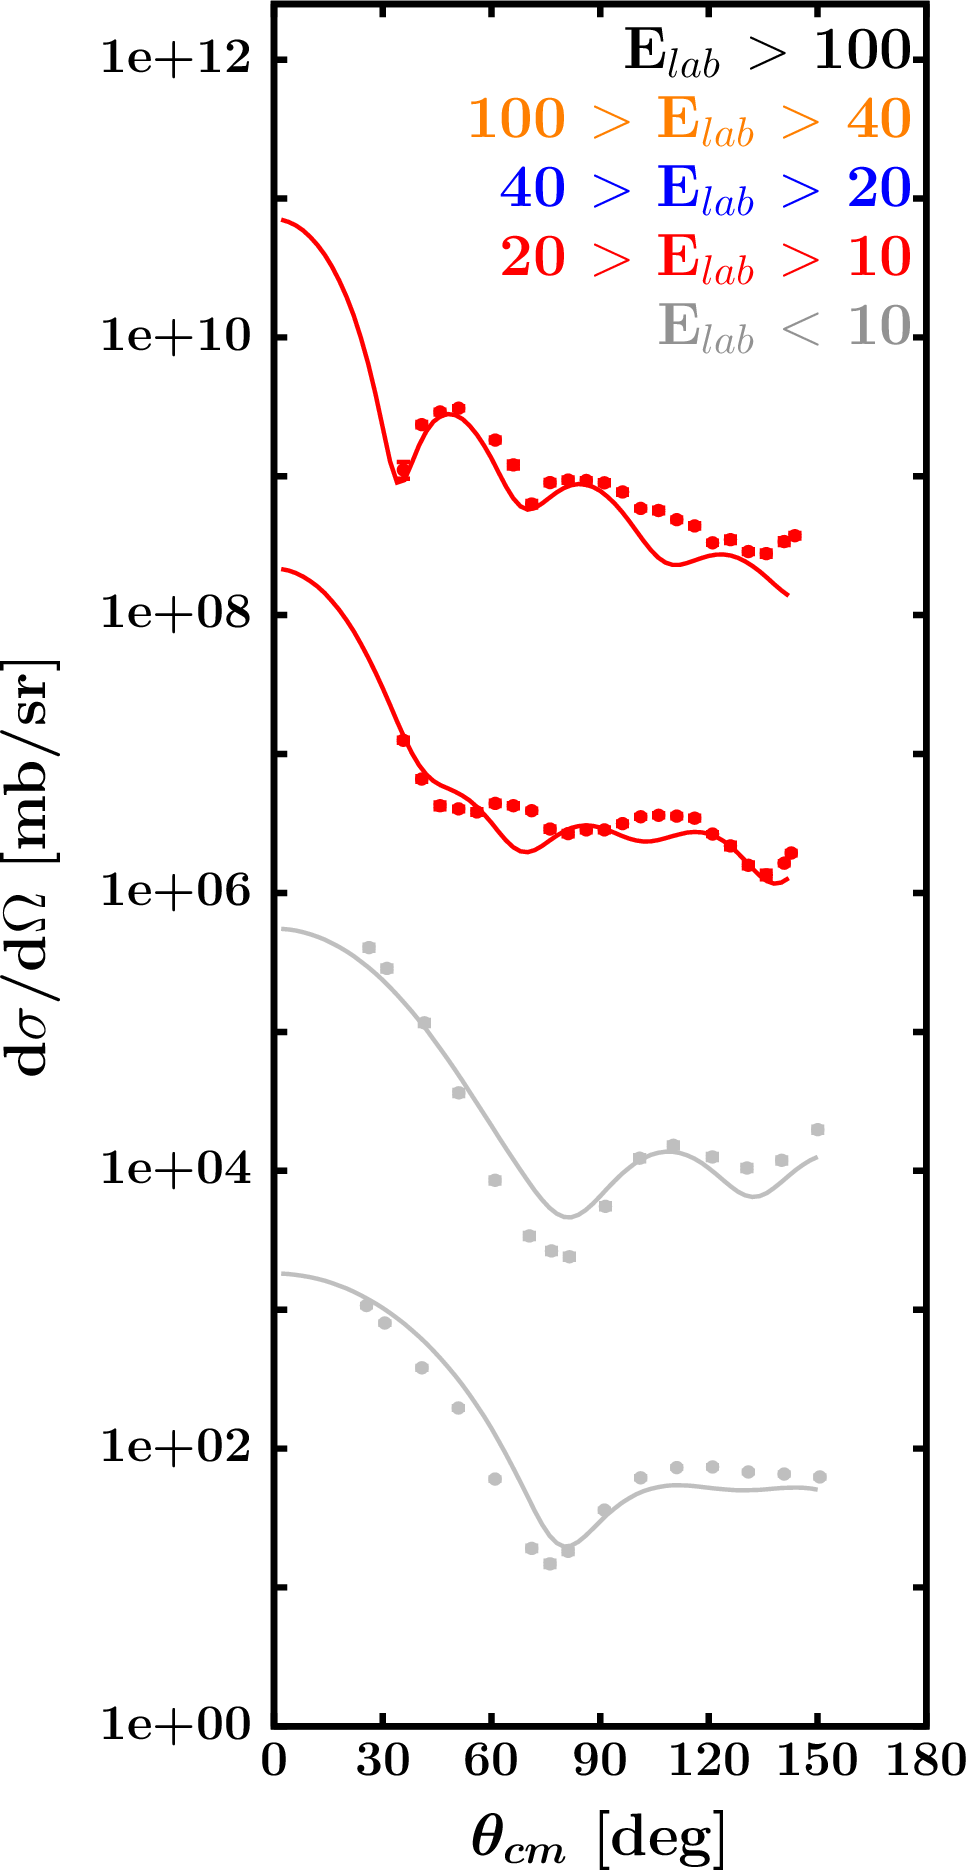
\includegraphics[width=1.0\textwidth]{figures/ca48_neutronElastic.png}
        \caption{Neutron elastic scattering data}
        \label{DOMFitData_ca48_neutron_elastic}
    \end{minipage}
\end{figure}

\begin{figure}[H]
    \centering
    \begin{minipage}{0.45\textwidth}
        \centering
        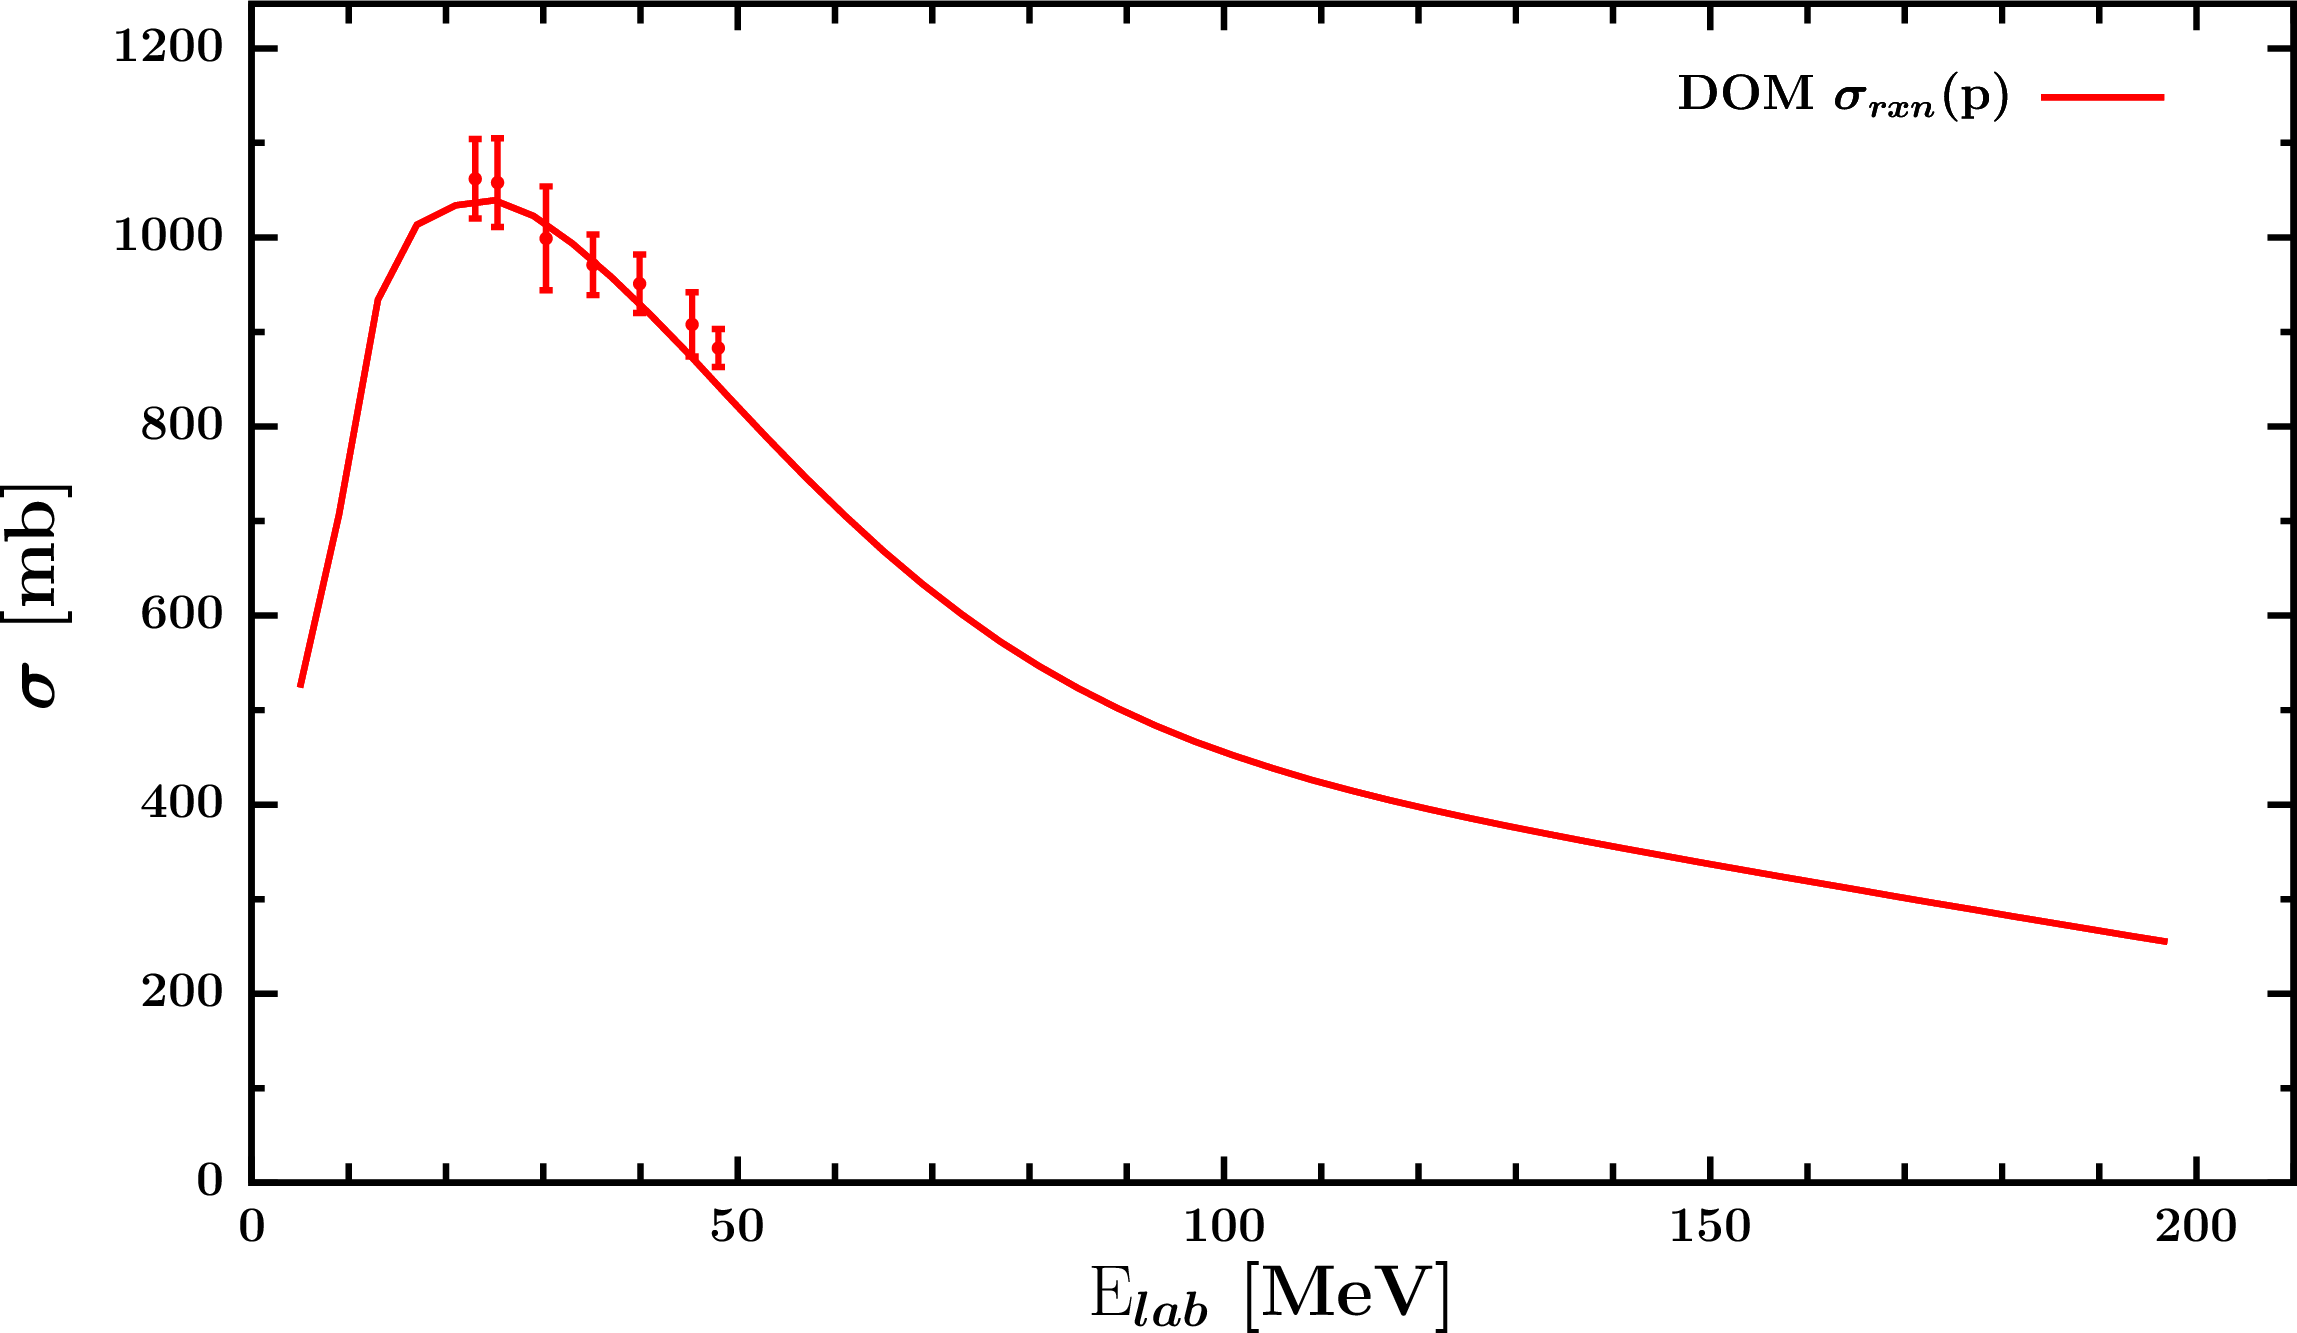
\includegraphics[width=1.0\textwidth]{figures/ca48_protonInelastic.png}
        \caption{Proton \rxn data}
        \label{DOMFitData_ca48_proton_inelastic}
    \end{minipage}\hfill
    \begin{minipage}{0.45\textwidth}
        \centering
        \includegraphics[width=1.0\textwidth]{figures/ca48_neutronInelastic.png}
        \caption{Neutron \rxn and \tot data}
        \label{DOMFitData_ca48_neutron_inelastic}
    \end{minipage}
\end{figure}

\afterpage{\clearpage}

\begin{figure}[H]
    \centering
    \begin{minipage}{0.45\textwidth}
        \centering
        \includegraphics[width=1.0\textwidth]{figures/ca48_chargeDensity.png}
        \caption{Charge density data}
        \label{DOMFitData_ca48_chargeDensity}
    \end{minipage}\hfill
    \begin{minipage}{0.45\textwidth}
        \centering
        \includegraphics[width=1.0\textwidth]{figures/ca48_SPLevels.png}
        \caption{Single-particle levels}
        \label{DOMFitData_ca48_SPLevels}
    \end{minipage}
\end{figure}

\afterpage{\clearpage}

\begin{figure}[H]
    \centering
    \begin{minipage}{0.45\textwidth}
        \centering
        \includegraphics[width=1.0\textwidth]{figures/ca48_protonPotentials.png}
        \caption{Energy-dependence of optical potential components for protons
        on \caEight}
        \label{DOMFitData_ca48_proton_potentialComponent_energy}
    \end{minipage}\hfill
    \begin{minipage}{0.45\textwidth}
        \centering
        \includegraphics[width=1.0\textwidth]{figures/ca48_neutronPotentials.png}
        \caption{Neutron potential energy-dependent component}
        \label{DOMFitData_ca48_neutron_potentialComponent_energy}
    \end{minipage}
\end{figure}

\begin{figure}[H]
    \centering
    \begin{minipage}{0.45\textwidth}
        \centering
        \includegraphics[width=1.0\textwidth]{figures/ca48_protonVolumeIntegrals.png}
        \caption{Proton potential, integrated over r-space}
        \label{DOMFitData_ca48_proton_potentialIntegral}
    \end{minipage}\hfill
    \begin{minipage}{0.45\textwidth}
        \centering
        \includegraphics[width=1.0\textwidth]{figures/ca48_neutronVolumeIntegrals.png}
        \caption{Neutron potential, integrated over r-space}
        \label{DOMFitData_ca48_neutron_potentialIntegral}
    \end{minipage}
\end{figure}

\afterpage{\clearpage}

\begin{figure}[H]
    \centering
    \begin{minipage}{0.45\textwidth}
        \centering
        \includegraphics[width=1.0\textwidth]{figures/ca48_protonSpectralFunctions.png}
        \caption{Proton spectral functions}
        \label{DOMFitData_ca48_proton_spectralFunctions}
    \end{minipage}\hfill
    \begin{minipage}{0.45\textwidth}
        \centering
        \includegraphics[width=1.0\textwidth]{figures/ca48_neutronSpectralFunctions.png}
        \caption{Neutron spectral functions}
        \label{DOMFitData_ca48_neutron_spectralFunctions}
    \end{minipage}
\end{figure}

\begin{figure}[H]
    \centering
    \includegraphics[width = 0.5\textwidth]{figures/ca48_matterDensity.png}
    \caption{Matter density distribution}
    \label{DOMFitData_ca48_matterDensity}
\end{figure}

\begin{figure}[H]
    \centering
    \includegraphics[width = 0.5\textwidth]{figures/ca48_momentumDistribution.png}
    \caption{Momentum distribution}
    \label{DOMFitData_ca48_momentumDistribution}
\end{figure}

\begin{figure}[H]
    \centering
    \includegraphics[width = 0.5\textwidth]{figures/ca48_energyDensity.png}
    \caption{Energy density distribution}
    \label{DOMFitData_ca48_energyDensity}
\end{figure}

\section{DOM fit of \niEight}

\label{ni58DOMOutput}
\begin{figure}[H]
    \centering
    \begin{minipage}{0.45\textwidth}
        \centering
        \includegraphics[width=1.0\textwidth]{figures/ni58_protonElastic.png}
        \caption{Proton elastic scattering data}
        \label{DOMFitData_ni58_proton_elastic}
    \end{minipage}\hfill
    \begin{minipage}{0.45\textwidth}
        \centering
        \includegraphics[width=1.0\textwidth]{figures/ni58_neutronElastic.png}
        \caption{Neutron elastic scattering data}
        \label{DOMFitData_ni58_neutron_elastic}
    \end{minipage}
\end{figure}

\begin{figure}[H]
    \centering
    \begin{minipage}{0.45\textwidth}
        \centering
        \includegraphics[width=1.0\textwidth]{figures/ni58_protonInelastic.png}
        \caption{Proton \rxn data}
        \label{DOMFitData_ni58_proton_inelastic}
    \end{minipage}\hfill
    \begin{minipage}{0.45\textwidth}
        \centering
        \includegraphics[width=1.0\textwidth]{figures/ni58_neutronInelastic.png}
        \caption{Neutron \rxn and \tot data}
        \label{DOMFitData_ni58_neutron_inelastic}
    \end{minipage}
\end{figure}

\afterpage{\clearpage}

\begin{figure}[H]
    \centering
    \begin{minipage}{0.45\textwidth}
        \centering
        \includegraphics[width=1.0\textwidth]{figures/ni58_chargeDensity.png}
        \caption{Charge density data}
        \label{DOMFitData_ni58_chargeDensity}
    \end{minipage}\hfill
    \begin{minipage}{0.45\textwidth}
        \centering
        \includegraphics[width=1.0\textwidth]{figures/ni58_SPLevels.png}
        \caption{Single-particle levels}
        \label{DOMFitData_ni58_SPLevels}
    \end{minipage}
\end{figure}

\afterpage{\clearpage}

\begin{figure}[H]
    \centering
    \begin{minipage}{0.45\textwidth}
        \centering
        \includegraphics[width=1.0\textwidth]{figures/ni58_protonPotentials.png}
        \caption{Energy-dependence of optical potential components for protons
        on \niEight}
        \label{DOMFitData_ni58_proton_potentialComponent_energy}
    \end{minipage}\hfill
    \begin{minipage}{0.45\textwidth}
        \centering
        \includegraphics[width=1.0\textwidth]{figures/ni58_neutronPotentials.png}
        \caption{Neutron potential energy-dependent component}
        \label{DOMFitData_ni58_neutron_potentialComponent_energy}
    \end{minipage}
\end{figure}

\begin{figure}[H]
    \centering
    \begin{minipage}{0.45\textwidth}
        \centering
        \includegraphics[width=1.0\textwidth]{figures/ni58_protonVolumeIntegrals.png}
        \caption{Proton potential, integrated over r-space}
        \label{DOMFitData_ni58_proton_potentialIntegral}
    \end{minipage}\hfill
    \begin{minipage}{0.45\textwidth}
        \centering
        \includegraphics[width=1.0\textwidth]{figures/ni58_neutronVolumeIntegrals.png}
        \caption{Neutron potential, integrated over r-space}
        \label{DOMFitData_ni58_neutron_potentialIntegral}
    \end{minipage}
\end{figure}

\afterpage{\clearpage}

\begin{figure}[H]
    \centering
    \begin{minipage}{0.45\textwidth}
        \centering
        \includegraphics[width=1.0\textwidth]{figures/ni58_protonSpectralFunctions.png}
        \caption{Proton spectral functions}
        \label{DOMFitData_ni58_proton_spectralFunctions}
    \end{minipage}\hfill
    \begin{minipage}{0.45\textwidth}
        \centering
        \includegraphics[width=1.0\textwidth]{figures/ni58_neutronSpectralFunctions.png}
        \caption{Neutron spectral functions}
        \label{DOMFitData_ni58_neutron_spectralFunctions}
    \end{minipage}
\end{figure}

\begin{figure}[H]
    \centering
    \includegraphics[width = 0.5\textwidth]{figures/ni58_matterDensity.png}
    \caption{Matter density distribution}
    \label{DOMFitData_ni58_matterDensity}
\end{figure}

\begin{figure}[H]
    \centering
    \includegraphics[width = 0.5\textwidth]{figures/ni58_momentumDistribution.png}
    \caption{Momentum distribution}
    \label{DOMFitData_ni58_momentumDistribution}
\end{figure}

\begin{figure}[H]
    \centering
    \includegraphics[width = 0.5\textwidth]{figures/ni58_energyDensity.png}
    \caption{Energy density distribution}
    \label{DOMFitData_ni58_energyDensity}
\end{figure}

\section{DOM fit of \niFour}

\label{ni64DOMOutput}
\begin{figure}[H]
    \centering
    \begin{minipage}{0.45\textwidth}
        \centering
        \includegraphics[width=1.0\textwidth]{figures/ni64_protonElastic.png}
        \caption{Proton elastic scattering data}
        \label{DOMFitData_ni64_proton_elastic}
    \end{minipage}\hfill
    \begin{minipage}{0.45\textwidth}
        \centering
        \includegraphics[width=1.0\textwidth]{figures/ni64_neutronElastic.png}
        \caption{Neutron elastic scattering data}
        \label{DOMFitData_ni64_neutron_elastic}
    \end{minipage}
\end{figure}

\begin{figure}[H]
    \centering
    \begin{minipage}{0.45\textwidth}
        \centering
        \includegraphics[width=1.0\textwidth]{figures/ni64_protonInelastic.png}
        \caption{Proton \rxn data}
        \label{DOMFitData_ni64_proton_inelastic}
    \end{minipage}\hfill
    \begin{minipage}{0.45\textwidth}
        \centering
        \includegraphics[width=1.0\textwidth]{figures/ni64_neutronInelastic.png}
        \caption{Neutron \rxn and \tot data}
        \label{DOMFitData_ni64_neutron_inelastic}
    \end{minipage}
\end{figure}

\afterpage{\clearpage}

\begin{figure}[H]
    \centering
    \begin{minipage}{0.45\textwidth}
        \centering
        \includegraphics[width=1.0\textwidth]{figures/ni64_chargeDensity.png}
        \caption{Charge density data}
        \label{DOMFitData_ni64_chargeDensity}
    \end{minipage}\hfill
    \begin{minipage}{0.45\textwidth}
        \centering
        \includegraphics[width=1.0\textwidth]{figures/ni64_SPLevels.png}
        \caption{Single-particle levels}
        \label{DOMFitData_ni64_SPLevels}
    \end{minipage}
\end{figure}

\afterpage{\clearpage}

\begin{figure}[H]
    \centering
    \begin{minipage}{0.45\textwidth}
        \centering
        \includegraphics[width=1.0\textwidth]{figures/ni64_protonPotentials.png}
        \caption{Energy-dependence of optical potential components for protons
        on \niFour}
        \label{DOMFitData_ni64_proton_potentialComponent_energy}
    \end{minipage}\hfill
    \begin{minipage}{0.45\textwidth}
        \centering
        \includegraphics[width=1.0\textwidth]{figures/ni64_neutronPotentials.png}
        \caption{Neutron potential energy-dependent component}
        \label{DOMFitData_ni64_neutron_potentialComponent_energy}
    \end{minipage}
\end{figure}

\begin{figure}[H]
    \centering
    \begin{minipage}{0.45\textwidth}
        \centering
        \includegraphics[width=1.0\textwidth]{figures/ni64_protonVolumeIntegrals.png}
        \caption{Proton potential, integrated over r-space}
        \label{DOMFitData_ni64_proton_potentialIntegral}
    \end{minipage}\hfill
    \begin{minipage}{0.45\textwidth}
        \centering
        \includegraphics[width=1.0\textwidth]{figures/ni64_neutronVolumeIntegrals.png}
        \caption{Neutron potential, integrated over r-space}
        \label{DOMFitData_ni64_neutron_potentialIntegral}
    \end{minipage}
\end{figure}

\afterpage{\clearpage}

\begin{figure}[H]
    \centering
    \begin{minipage}{0.45\textwidth}
        \centering
        \includegraphics[width=1.0\textwidth]{figures/ni64_protonSpectralFunctions.png}
        \caption{Proton spectral functions}
        \label{DOMFitData_ni64_proton_spectralFunctions}
    \end{minipage}\hfill
    \begin{minipage}{0.45\textwidth}
        \centering
        \includegraphics[width=1.0\textwidth]{figures/ni64_neutronSpectralFunctions.png}
        \caption{Neutron spectral functions}
        \label{DOMFitData_ni64_neutron_spectralFunctions}
    \end{minipage}
\end{figure}

\begin{figure}[H]
    \centering
    \includegraphics[width = 0.5\textwidth]{figures/ni64_matterDensity.png}
    \caption{Matter density distribution}
    \label{DOMFitData_ni64_matterDensity}
\end{figure}

\begin{figure}[H]
    \centering
    \includegraphics[width = 0.5\textwidth]{figures/ni64_momentumDistribution.png}
    \caption{Momentum distribution}
    \label{DOMFitData_ni64_momentumDistribution}
\end{figure}

\begin{figure}[H]
    \centering
    \includegraphics[width = 0.5\textwidth]{figures/ni64_energyDensity.png}
    \caption{Energy density distribution}
    \label{DOMFitData_ni64_energyDensity}
\end{figure}

\section{DOM fit of \snTwelve}

\label{sn112DOMOutput}
\begin{figure}[H]
    \centering
    \begin{minipage}{0.45\textwidth}
        \centering
        \includegraphics[width=1.0\textwidth]{figures/sn112_protonElastic.png}
        \caption{Proton elastic scattering data}
        \label{DOMFitData_sn112_proton_elastic}
    \end{minipage}\hfill
    \begin{minipage}{0.45\textwidth}
        \centering
        \includegraphics[width=1.0\textwidth]{figures/sn112_neutronElastic.png}
        \caption{Neutron elastic scattering data}
        \label{DOMFitData_sn112_neutron_elastic}
    \end{minipage}
\end{figure}

\begin{figure}[H]
    \centering
    \begin{minipage}{0.45\textwidth}
        \centering
        \includegraphics[width=1.0\textwidth]{figures/sn112_protonInelastic.png}
        \caption{Proton \rxn data}
        \label{DOMFitData_sn112_proton_inelastic}
    \end{minipage}\hfill
    \begin{minipage}{0.45\textwidth}
        \centering
        \includegraphics[width=1.0\textwidth]{figures/sn112_neutronInelastic.png}
        \caption{Neutron \rxn and \tot data}
        \label{DOMFitData_sn112_neutron_inelastic}
    \end{minipage}
\end{figure}

\afterpage{\clearpage}

\begin{figure}[H]
    \centering
    \begin{minipage}{0.45\textwidth}
        \centering
        \includegraphics[width=1.0\textwidth]{figures/sn112_chargeDensity.png}
        \caption{Charge density data}
        \label{DOMFitData_sn112_chargeDensity}
    \end{minipage}\hfill
    \begin{minipage}{0.45\textwidth}
        \centering
        \includegraphics[width=1.0\textwidth]{figures/sn112_SPLevels.png}
        \caption{Single-particle levels}
        \label{DOMFitData_sn112_SPLevels}
    \end{minipage}
\end{figure}

\afterpage{\clearpage}

\begin{figure}[H]
    \centering
    \begin{minipage}{0.45\textwidth}
        \centering
        \includegraphics[width=1.0\textwidth]{figures/sn112_protonPotentials.png}
        \caption{Energy-dependence of optical potential components for protons
        on \snTwelve}
        \label{DOMFitData_sn112_proton_potentialComponent_energy}
    \end{minipage}\hfill
    \begin{minipage}{0.45\textwidth}
        \centering
        \includegraphics[width=1.0\textwidth]{figures/sn112_neutronPotentials.png}
        \caption{Neutron potential energy-dependent component}
        \label{DOMFitData_sn112_neutron_potentialComponent_energy}
    \end{minipage}
\end{figure}

\begin{figure}[H]
    \centering
    \begin{minipage}{0.45\textwidth}
        \centering
        \includegraphics[width=1.0\textwidth]{figures/sn112_protonVolumeIntegrals.png}
        \caption{Proton potential, integrated over r-space}
        \label{DOMFitData_sn112_proton_potentialIntegral}
    \end{minipage}\hfill
    \begin{minipage}{0.45\textwidth}
        \centering
        \includegraphics[width=1.0\textwidth]{figures/sn112_neutronVolumeIntegrals.png}
        \caption{Neutron potential, integrated over r-space}
        \label{DOMFitData_sn112_neutron_potentialIntegral}
    \end{minipage}
\end{figure}

\afterpage{\clearpage}

\begin{figure}[H]
    \centering
    \begin{minipage}{0.45\textwidth}
        \centering
        \includegraphics[width=1.0\textwidth]{figures/sn112_protonSpectralFunctions.png}
        \caption{Proton spectral functions}
        \label{DOMFitData_sn112_proton_spectralFunctions}
    \end{minipage}\hfill
    \begin{minipage}{0.45\textwidth}
        \centering
        \includegraphics[width=1.0\textwidth]{figures/sn112_neutronSpectralFunctions.png}
        \caption{Neutron spectral functions}
        \label{DOMFitData_sn112_neutron_spectralFunctions}
    \end{minipage}
\end{figure}

\begin{figure}[H]
    \centering
    \includegraphics[width = 0.5\textwidth]{figures/sn112_matterDensity.png}
    \caption{Matter density distribution}
    \label{DOMFitData_sn112_matterDensity}
\end{figure}

\begin{figure}[H]
    \centering
    \includegraphics[width = 0.5\textwidth]{figures/sn112_momentumDistribution.png}
    \caption{Momentum distribution}
    \label{DOMFitData_sn112_momentumDistribution}
\end{figure}

\begin{figure}[H]
    \centering
    \includegraphics[width = 0.5\textwidth]{figures/sn112_energyDensity.png}
    \caption{Energy density distribution}
    \label{DOMFitData_sn112_energyDensity}
\end{figure}

\section{DOM fit of \snFour}

\label{sn124DOMOutput}
\begin{figure}[H]
    \centering
    \begin{minipage}{0.45\textwidth}
        \centering
        \includegraphics[width=1.0\textwidth]{figures/sn124_protonElastic.png}
        \caption{Proton elastic scattering data}
        \label{DOMFitData_sn124_proton_elastic}
    \end{minipage}\hfill
    \begin{minipage}{0.45\textwidth}
        \centering
        \includegraphics[width=1.0\textwidth]{figures/sn124_neutronElastic.png}
        \caption{Neutron elastic scattering data}
        \label{DOMFitData_sn124_neutron_elastic}
    \end{minipage}
\end{figure}

\begin{figure}[H]
    \centering
    \begin{minipage}{0.45\textwidth}
        \centering
        \includegraphics[width=1.0\textwidth]{figures/sn124_protonInelastic.png}
        \caption{Proton \rxn data}
        \label{DOMFitData_sn124_proton_inelastic}
    \end{minipage}\hfill
    \begin{minipage}{0.45\textwidth}
        \centering
        \includegraphics[width=1.0\textwidth]{figures/sn124_neutronInelastic.png}
        \caption{Neutron \rxn and \tot data}
        \label{DOMFitData_sn124_neutron_inelastic}
    \end{minipage}
\end{figure}

\afterpage{\clearpage}

\begin{figure}[H]
    \centering
    \begin{minipage}{0.45\textwidth}
        \centering
        \includegraphics[width=1.0\textwidth]{figures/sn124_chargeDensity.png}
        \caption{Charge density data}
        \label{DOMFitData_sn124_chargeDensity}
    \end{minipage}\hfill
    \begin{minipage}{0.45\textwidth}
        \centering
        \includegraphics[width=1.0\textwidth]{figures/sn124_SPLevels.png}
        \caption{Single-particle levels}
        \label{DOMFitData_sn124_SPLevels}
    \end{minipage}
\end{figure}

\afterpage{\clearpage}

\begin{figure}[H]
    \centering
    \begin{minipage}{0.45\textwidth}
        \centering
        \includegraphics[width=1.0\textwidth]{figures/sn124_protonPotentials.png}
        \caption{Energy-dependence of optical potential components for protons
        on \snFour}
        \label{DOMFitData_sn124_proton_potentialComponent_energy}
    \end{minipage}\hfill
    \begin{minipage}{0.45\textwidth}
        \centering
        \includegraphics[width=1.0\textwidth]{figures/sn124_neutronPotentials.png}
        \caption{Neutron potential energy-dependent component}
        \label{DOMFitData_sn124_neutron_potentialComponent_energy}
    \end{minipage}
\end{figure}

\begin{figure}[H]
    \centering
    \begin{minipage}{0.45\textwidth}
        \centering
        \includegraphics[width=1.0\textwidth]{figures/sn124_protonVolumeIntegrals.png}
        \caption{Proton potential, integrated over r-space}
        \label{DOMFitData_sn124_proton_potentialIntegral}
    \end{minipage}\hfill
    \begin{minipage}{0.45\textwidth}
        \centering
        \includegraphics[width=1.0\textwidth]{figures/sn124_neutronVolumeIntegrals.png}
        \caption{Neutron potential, integrated over r-space}
        \label{DOMFitData_sn124_neutron_potentialIntegral}
    \end{minipage}
\end{figure}

\afterpage{\clearpage}

\begin{figure}[H]
    \centering
    \begin{minipage}{0.45\textwidth}
        \centering
        \includegraphics[width=1.0\textwidth]{figures/sn124_protonSpectralFunctions.png}
        \caption{Proton spectral functions}
        \label{DOMFitData_sn124_proton_spectralFunctions}
    \end{minipage}\hfill
    \begin{minipage}{0.45\textwidth}
        \centering
        \includegraphics[width=1.0\textwidth]{figures/sn124_neutronSpectralFunctions.png}
        \caption{Neutron spectral functions}
        \label{DOMFitData_sn124_neutron_spectralFunctions}
    \end{minipage}
\end{figure}

\begin{figure}[H]
    \centering
    \includegraphics[width = 0.5\textwidth]{figures/sn124_matterDensity.png}
    \caption{Matter density distribution}
    \label{DOMFitData_sn124_matterDensity}
\end{figure}

\begin{figure}[H]
    \centering
    \includegraphics[width = 0.5\textwidth]{figures/sn124_momentumDistribution.png}
    \caption{Momentum distribution}
    \label{DOMFitData_sn124_momentumDistribution}
\end{figure}

\begin{figure}[H]
    \centering
    \includegraphics[width = 0.5\textwidth]{figures/sn124_energyDensity.png}
    \caption{Energy density distribution}
    \label{DOMFitData_sn124_energyDensity}
\end{figure}

\section{DOM fit of \pbEight}

\label{pb208DOMOutput}
\begin{figure}[H]
    \centering
    \begin{minipage}{0.45\textwidth}
        \centering
        \includegraphics[width=1.0\textwidth]{figures/pb208_protonElastic.png}
        \caption{Proton elastic scattering data}
        \label{DOMFitData_pb208_proton_elastic}
    \end{minipage}\hfill
    \begin{minipage}{0.45\textwidth}
        \centering
        \includegraphics[width=1.0\textwidth]{figures/pb208_neutronElastic.png}
        \caption{Neutron elastic scattering data}
        \label{DOMFitData_pb208_neutron_elastic}
    \end{minipage}
\end{figure}

\begin{figure}[H]
    \centering
    \begin{minipage}{0.45\textwidth}
        \centering
        \includegraphics[width=1.0\textwidth]{figures/pb208_protonInelastic.png}
        \caption{Proton \rxn data}
        \label{DOMFitData_pb208_proton_inelastic}
    \end{minipage}\hfill
    \begin{minipage}{0.45\textwidth}
        \centering
        \includegraphics[width=1.0\textwidth]{figures/pb208_neutronInelastic.png}
        \caption{Neutron \rxn and \tot data}
        \label{DOMFitData_pb208_neutron_inelastic}
    \end{minipage}
\end{figure}

\afterpage{\clearpage}

\begin{figure}[H]
    \centering
    \begin{minipage}{0.45\textwidth}
        \centering
        \includegraphics[width=1.0\textwidth]{figures/pb208_chargeDensity.png}
        \caption{Charge density data}
        \label{DOMFitData_pb208_chargeDensity}
    \end{minipage}\hfill
    \begin{minipage}{0.45\textwidth}
        \centering
        \includegraphics[width=1.0\textwidth]{figures/pb208_SPLevels.png}
        \caption{Single-particle levels}
        \label{DOMFitData_pb208_SPLevels}
    \end{minipage}
\end{figure}

\afterpage{\clearpage}

\begin{figure}[H]
    \centering
    \begin{minipage}{0.45\textwidth}
        \centering
        \includegraphics[width=1.0\textwidth]{figures/pb208_protonPotentials.png}
        \caption{Energy-dependence of optical potential components for protons
        on \pbEight}
        \label{DOMFitData_pb208_proton_potentialComponent_energy}
    \end{minipage}\hfill
    \begin{minipage}{0.45\textwidth}
        \centering
        \includegraphics[width=1.0\textwidth]{figures/pb208_neutronPotentials.png}
        \caption{Neutron potential energy-dependent component}
        \label{DOMFitData_pb208_neutron_potentialComponent_energy}
    \end{minipage}
\end{figure}

\begin{figure}[H]
    \centering
    \begin{minipage}{0.45\textwidth}
        \centering
        \includegraphics[width=1.0\textwidth]{figures/pb208_protonVolumeIntegrals.png}
        \caption{Proton potential, integrated over r-space}
        \label{DOMFitData_pb208_proton_potentialIntegral}
    \end{minipage}\hfill
    \begin{minipage}{0.45\textwidth}
        \centering
        \includegraphics[width=1.0\textwidth]{figures/pb208_neutronVolumeIntegrals.png}
        \caption{Neutron potential, integrated over r-space}
        \label{DOMFitData_pb208_neutron_potentialIntegral}
    \end{minipage}
\end{figure}

\afterpage{\clearpage}

\begin{figure}[H]
    \centering
    \begin{minipage}{0.45\textwidth}
        \centering
        \includegraphics[width=1.0\textwidth]{figures/pb208_protonSpectralFunctions.png}
        \caption{Proton spectral functions}
        \label{DOMFitData_pb208_proton_spectralFunctions}
    \end{minipage}\hfill
    \begin{minipage}{0.45\textwidth}
        \centering
        \includegraphics[width=1.0\textwidth]{figures/pb208_neutronSpectralFunctions.png}
        \caption{Neutron spectral functions}
        \label{DOMFitData_pb208_neutron_spectralFunctions}
    \end{minipage}
\end{figure}

\begin{figure}[H]
    \centering
    \includegraphics[width = 0.5\textwidth]{figures/pb208_matterDensity.png}
    \caption{Matter density distribution}
    \label{DOMFitData_pb208_matterDensity}
\end{figure}

\begin{figure}[H]
    \centering
    \includegraphics[width = 0.5\textwidth]{figures/pb208_momentumDistribution.png}
    \caption{Momentum distribution}
    \label{DOMFitData_pb208_momentumDistribution}
\end{figure}

\begin{figure}[H]
    \centering
    \includegraphics[width = 0.5\textwidth]{figures/pb208_energyDensity.png}
    \caption{Energy density distribution}
    \label{DOMFitData_pb208_energyDensity}
\end{figure}

\end{figure}
